\documentclass{book}
\usepackage{amsmath, amsthm, amssymb, amsfonts}\usepackage{thmtools}\usepackage{parskip}\usepackage[pdftex]{graphicx}\usepackage[a4paper, margin=4cm]{geometry} % margins%
\usepackage{calc}\usepackage{setspace}\usepackage{geometry}\usepackage{float}\usepackage[hidelinks]{hyperref}\usepackage[utf8]{inputenc}\usepackage[english,danish]{babel}\usepackage{framed}\usepackage[dvipsnames,table]{xcolor} \usepackage{tcolorbox}\usepackage{hyperref}\usepackage{lastpage}\usepackage{fancyhdr}
%https://www.overleaf.com/learn/latex/Multiple_columns Linket her kan bruges til at indelle sider i kolumner
\usepackage{titlesec} %den her pakke bruges til at fjerne "Kapitel n" fra kapitelsidderne
\usepackage{minitoc}
\usepackage{gensymb} %Bruges til at kunne lave grader tegn
\usepackage{tcolorbox}
\usepackage{ifthen} % Skal bruges til sidebar
\usepackage{afterpage}
\renewcommand{\chaptermark}[1]{\markboth{#1}{}} % Fjerne kapitel nummeret fra headeren
\usepackage{tikz}
\titleformat{\chapter}[display] {\normalfont\huge\bfseries}{}{0pt}{\Huge} \pagestyle{fancy}
\fancyhf{} % Clear the header and footer
\fancyhead[LE,RO]{\thepage} % Page number on the outer (left on even, right on odd) side
\fancyhead[RE]{\leftmark} % Chapter title on the inner side (right on even pages)
\fancyhead[LO]{\leftmark} % Chapter title on the inner side (left on odd pages}
\definecolor{mahogany}{rgb}{192, 64, 0} % RGB for mahogany
\definecolor{gennemstegt}{rgb}{192, 112, 0}
\newcommand{\emptystar}{\textcolor{gray}{\textbf{$\star$}}}
\newcommand{\fullstar}{\textbf{$\star$}}

\title{Victors Kogebog med Stjålne Opskrifter}
\author{Victor Posselt Sandberg}
\date{\today}
\begin{document}
\dominitoc  

\frontmatter
\maketitle 
\begin{figure}
    \centering
    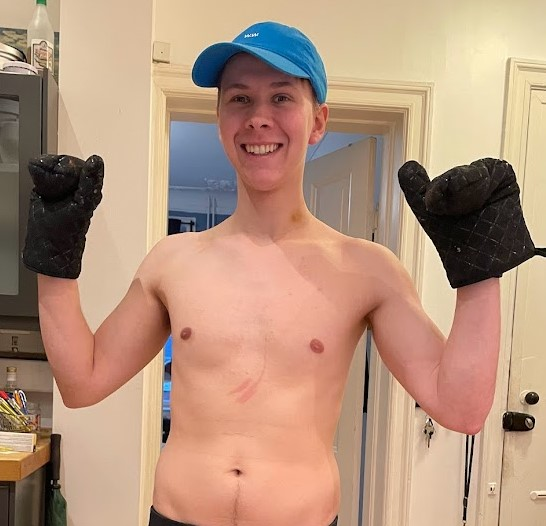
\includegraphics[width=1\linewidth]{Billeder/Mave2.jpg}
    \caption{Det mig}
\end{figure}
\newpage \tableofcontents
\mainmatter
\newpage\chapter{Introduktion} 
Gennem de sidste 2 år har jeg haft til mål at lave mindst en ny opskrift per måned. Dette har bragt mig rundt omkring med unikke, spændende og lækre opskrifter. Jeg håber at denne bog kan få nogle inspirationer og nogle lækre måltider frem. 
\\Bogen er stadig et work in progress, da dette mål med en ny ret vil fortsætte, og udover dette eksperimentere jge også med hvilket setup giver bedst mening for en bog.
\\ Der er i særdelles lagt vægt på 2 afsnit, aftensmad og brød. Dette skyldes at det især har været disse 2 felter jeg indtil videre har udforsket, den nuværende fordeling er subject to change, men indtil videre, alfabetisk opdelling inden for hver kapitel, med vegetarisk og ikke-vegetraisk fordeling i aftensmaden. \\ Som udganspunkt har jeg prøvet at undgå at bruge halve mål i mine opskrifter, da det giver en mere naturlig opdelling og mulighed for opskalleringen med hele tal. I de tilfælde hvor der er halve eller ligende, har jeg forsøgt at bruge brøkker frem fra komma tal da jeg bruger "." som seperattor frem for ",". 
\\ \\ \textbf{Bon Appetit} 
\chapter{Morgenmad}
\minitoc
%\newpage \section{Bananpandekager}
\newpage \section{French Toast}
\begin{minipage}[t]{0.5\textwidth}
\textbf{Ingredienser:}
\begin{itemize}
    \item 1 Toastbrød (helst et i en fin størrelse, såsom multikernebrød fra Netto)
    \item 1 æg
    \item Eventuelt
    \begin{itemize}
        \item En skive ost
        \item Et stykke skinke
        \item Endnu et stykke toastbrød
        \item Forårsløg til pynt
    \end{itemize}
\end{itemize}
\end{minipage}
\begin{minipage}[t]{0.5\textwidth}
\textbf{Fremgangsmåde:}
\begin{enumerate}
    \item Skær en stykke af brødet ud fra midten, således ægget kan klægges deri.
    \item Steg på en pande, eventuelt med "låg".
    \item Hvis man vil have det som en pariser toast agitg, så lig ost, skinke og det andet stykke brød på.
    \item Lad brødet blive gylden brunt og vend
\end{enumerate}
\end{minipage}
\newpage \begin{tikzpicture}[remember picture,overlay,inner sep=0pt,outer sep=0pt]
    \node[anchor=south east] at (current page.south east) {
        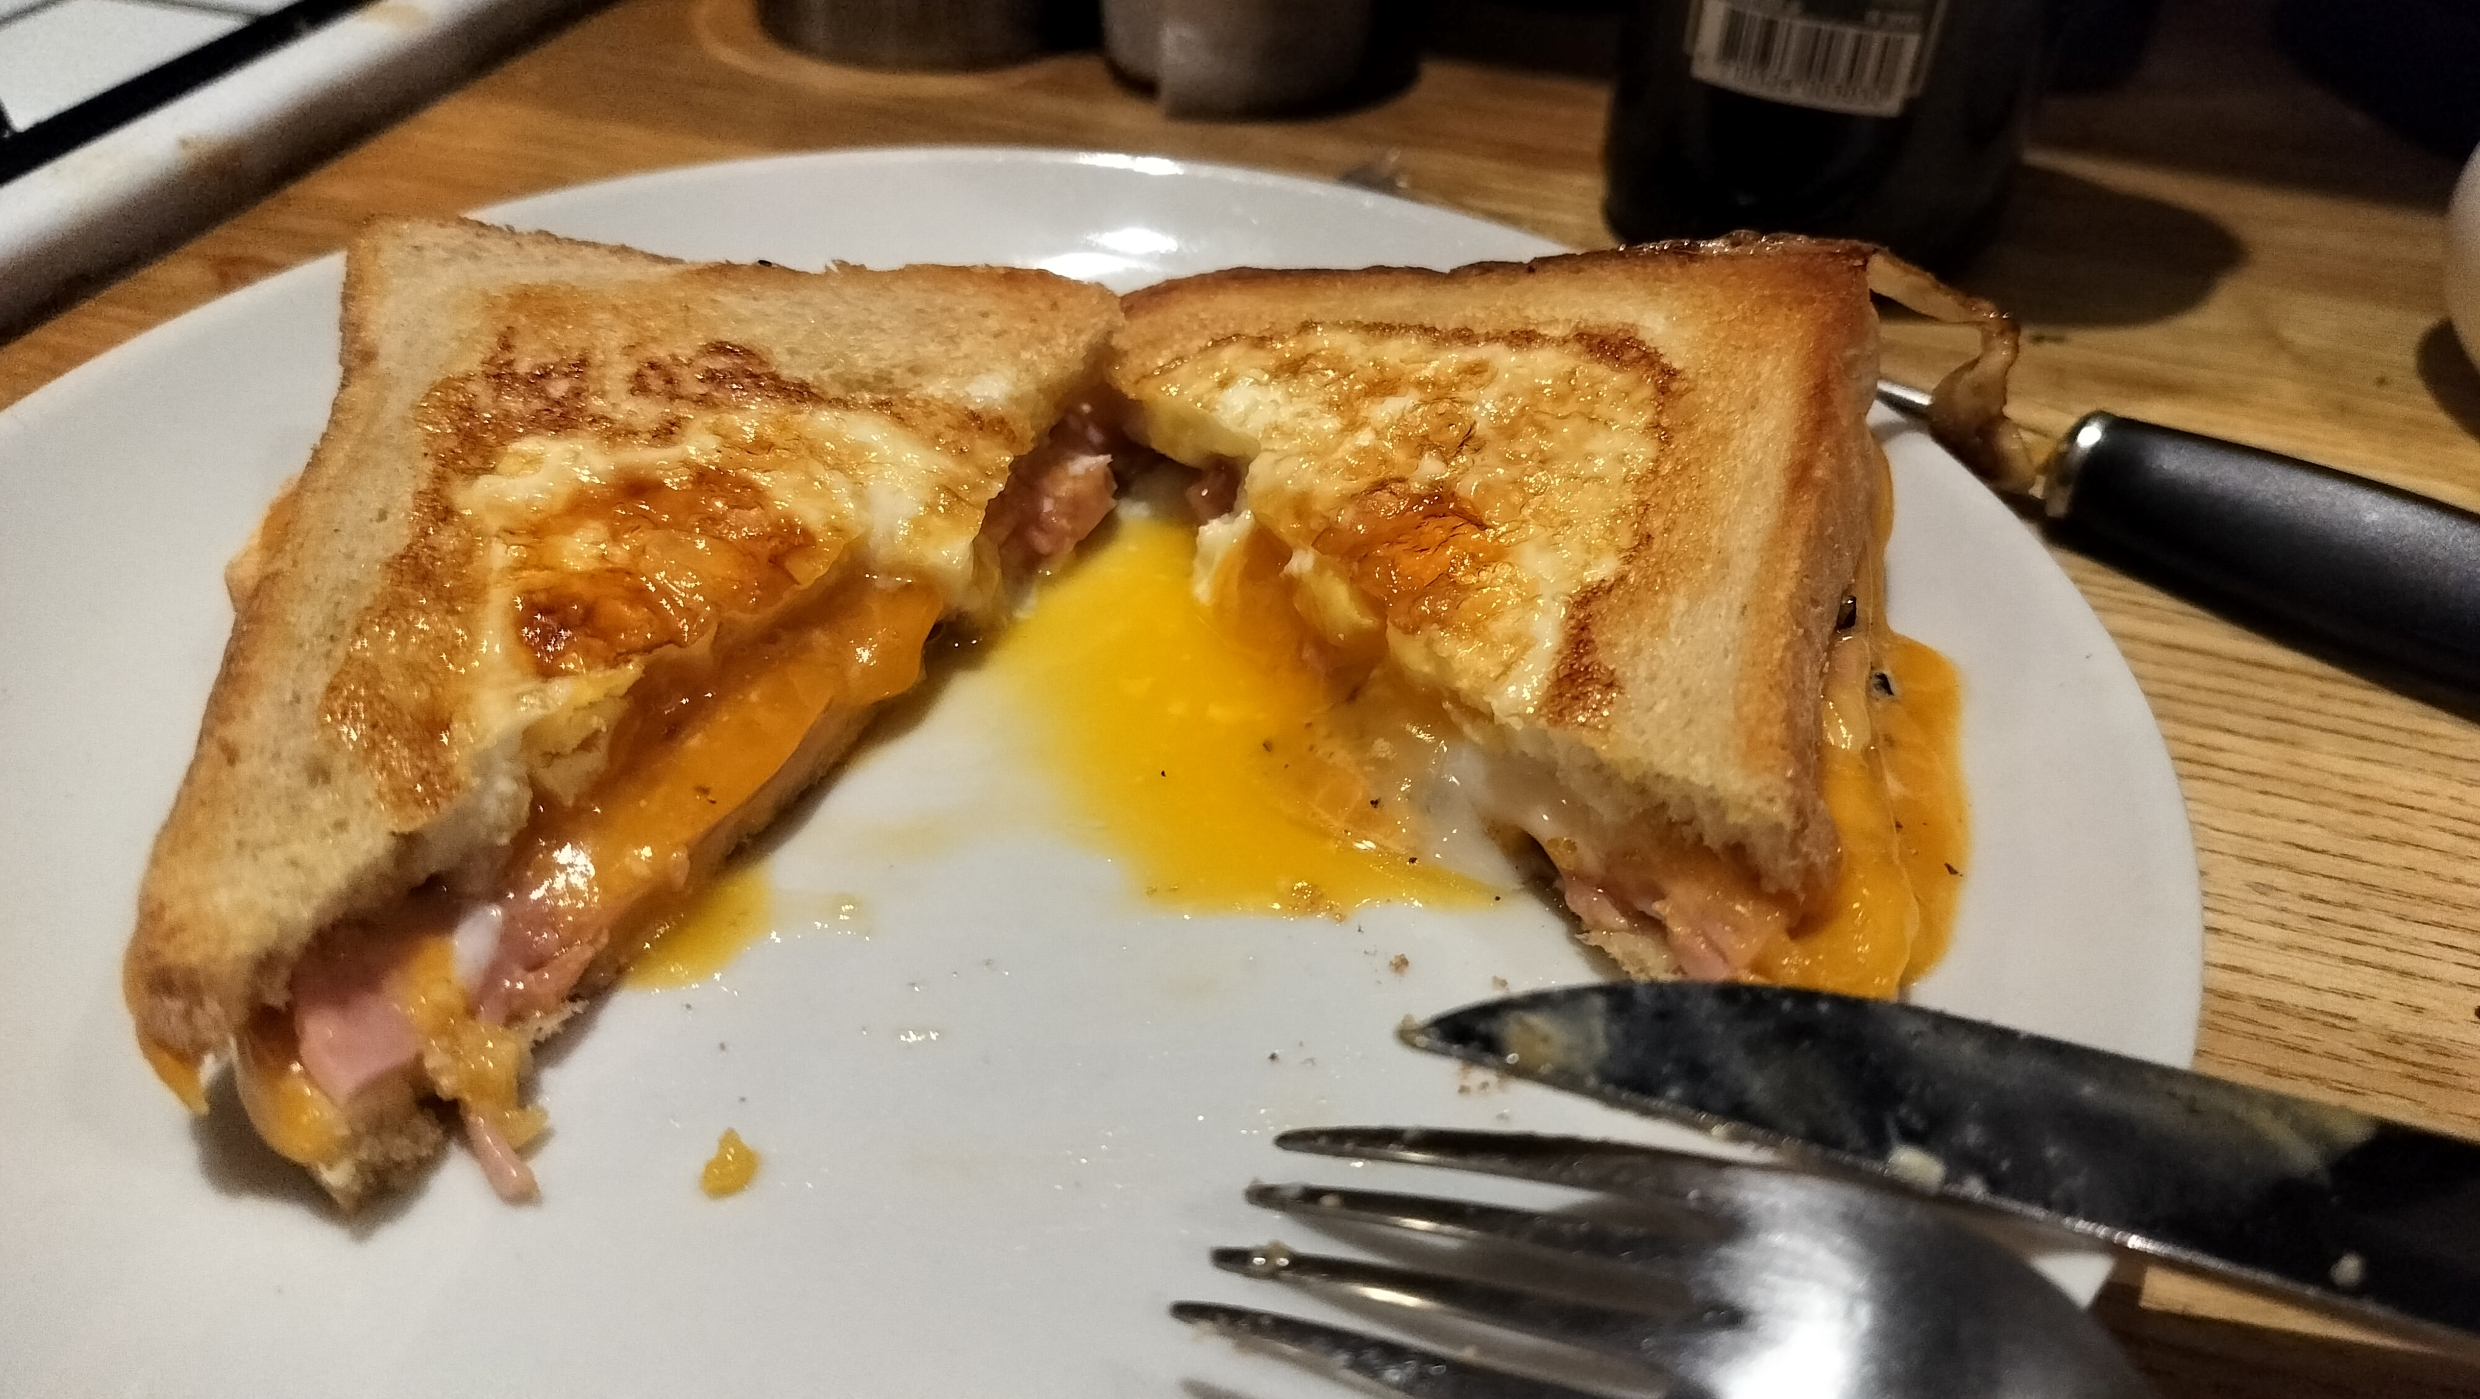
\includegraphics[width=\paperwidth,height=\paperheight]{Billeder/Morgenmad/French_Toast2.jpg}
    };
\end{tikzpicture}
\clearpage \section{Røræg}
\begin{minipage}[t]{0.5\textwidth}
 - 4 æg
\\ - 100 g cremfraice eller græsk yoghurt
\\ Salt, pebber og evt. timian
\end{minipage}
\begin{minipage}[t]{0.5\textwidth}
 \textbf{Fremgansmåde:}
\begin{enumerate}
    \item Bland æggene og mælkeproduktet sammen til en ensformig masse. 
    \item Steg på panden ved lav varme.
    OBS. Der kan med fordel vendes med en spise pind da det giver mindre smuldrende æg.
\end{enumerate}
\end{minipage}
\newpage \begin{tikzpicture}[remember picture,overlay,inner sep=0pt,outer sep=0pt]
    \node[anchor=south east] at (current page.south east) {
        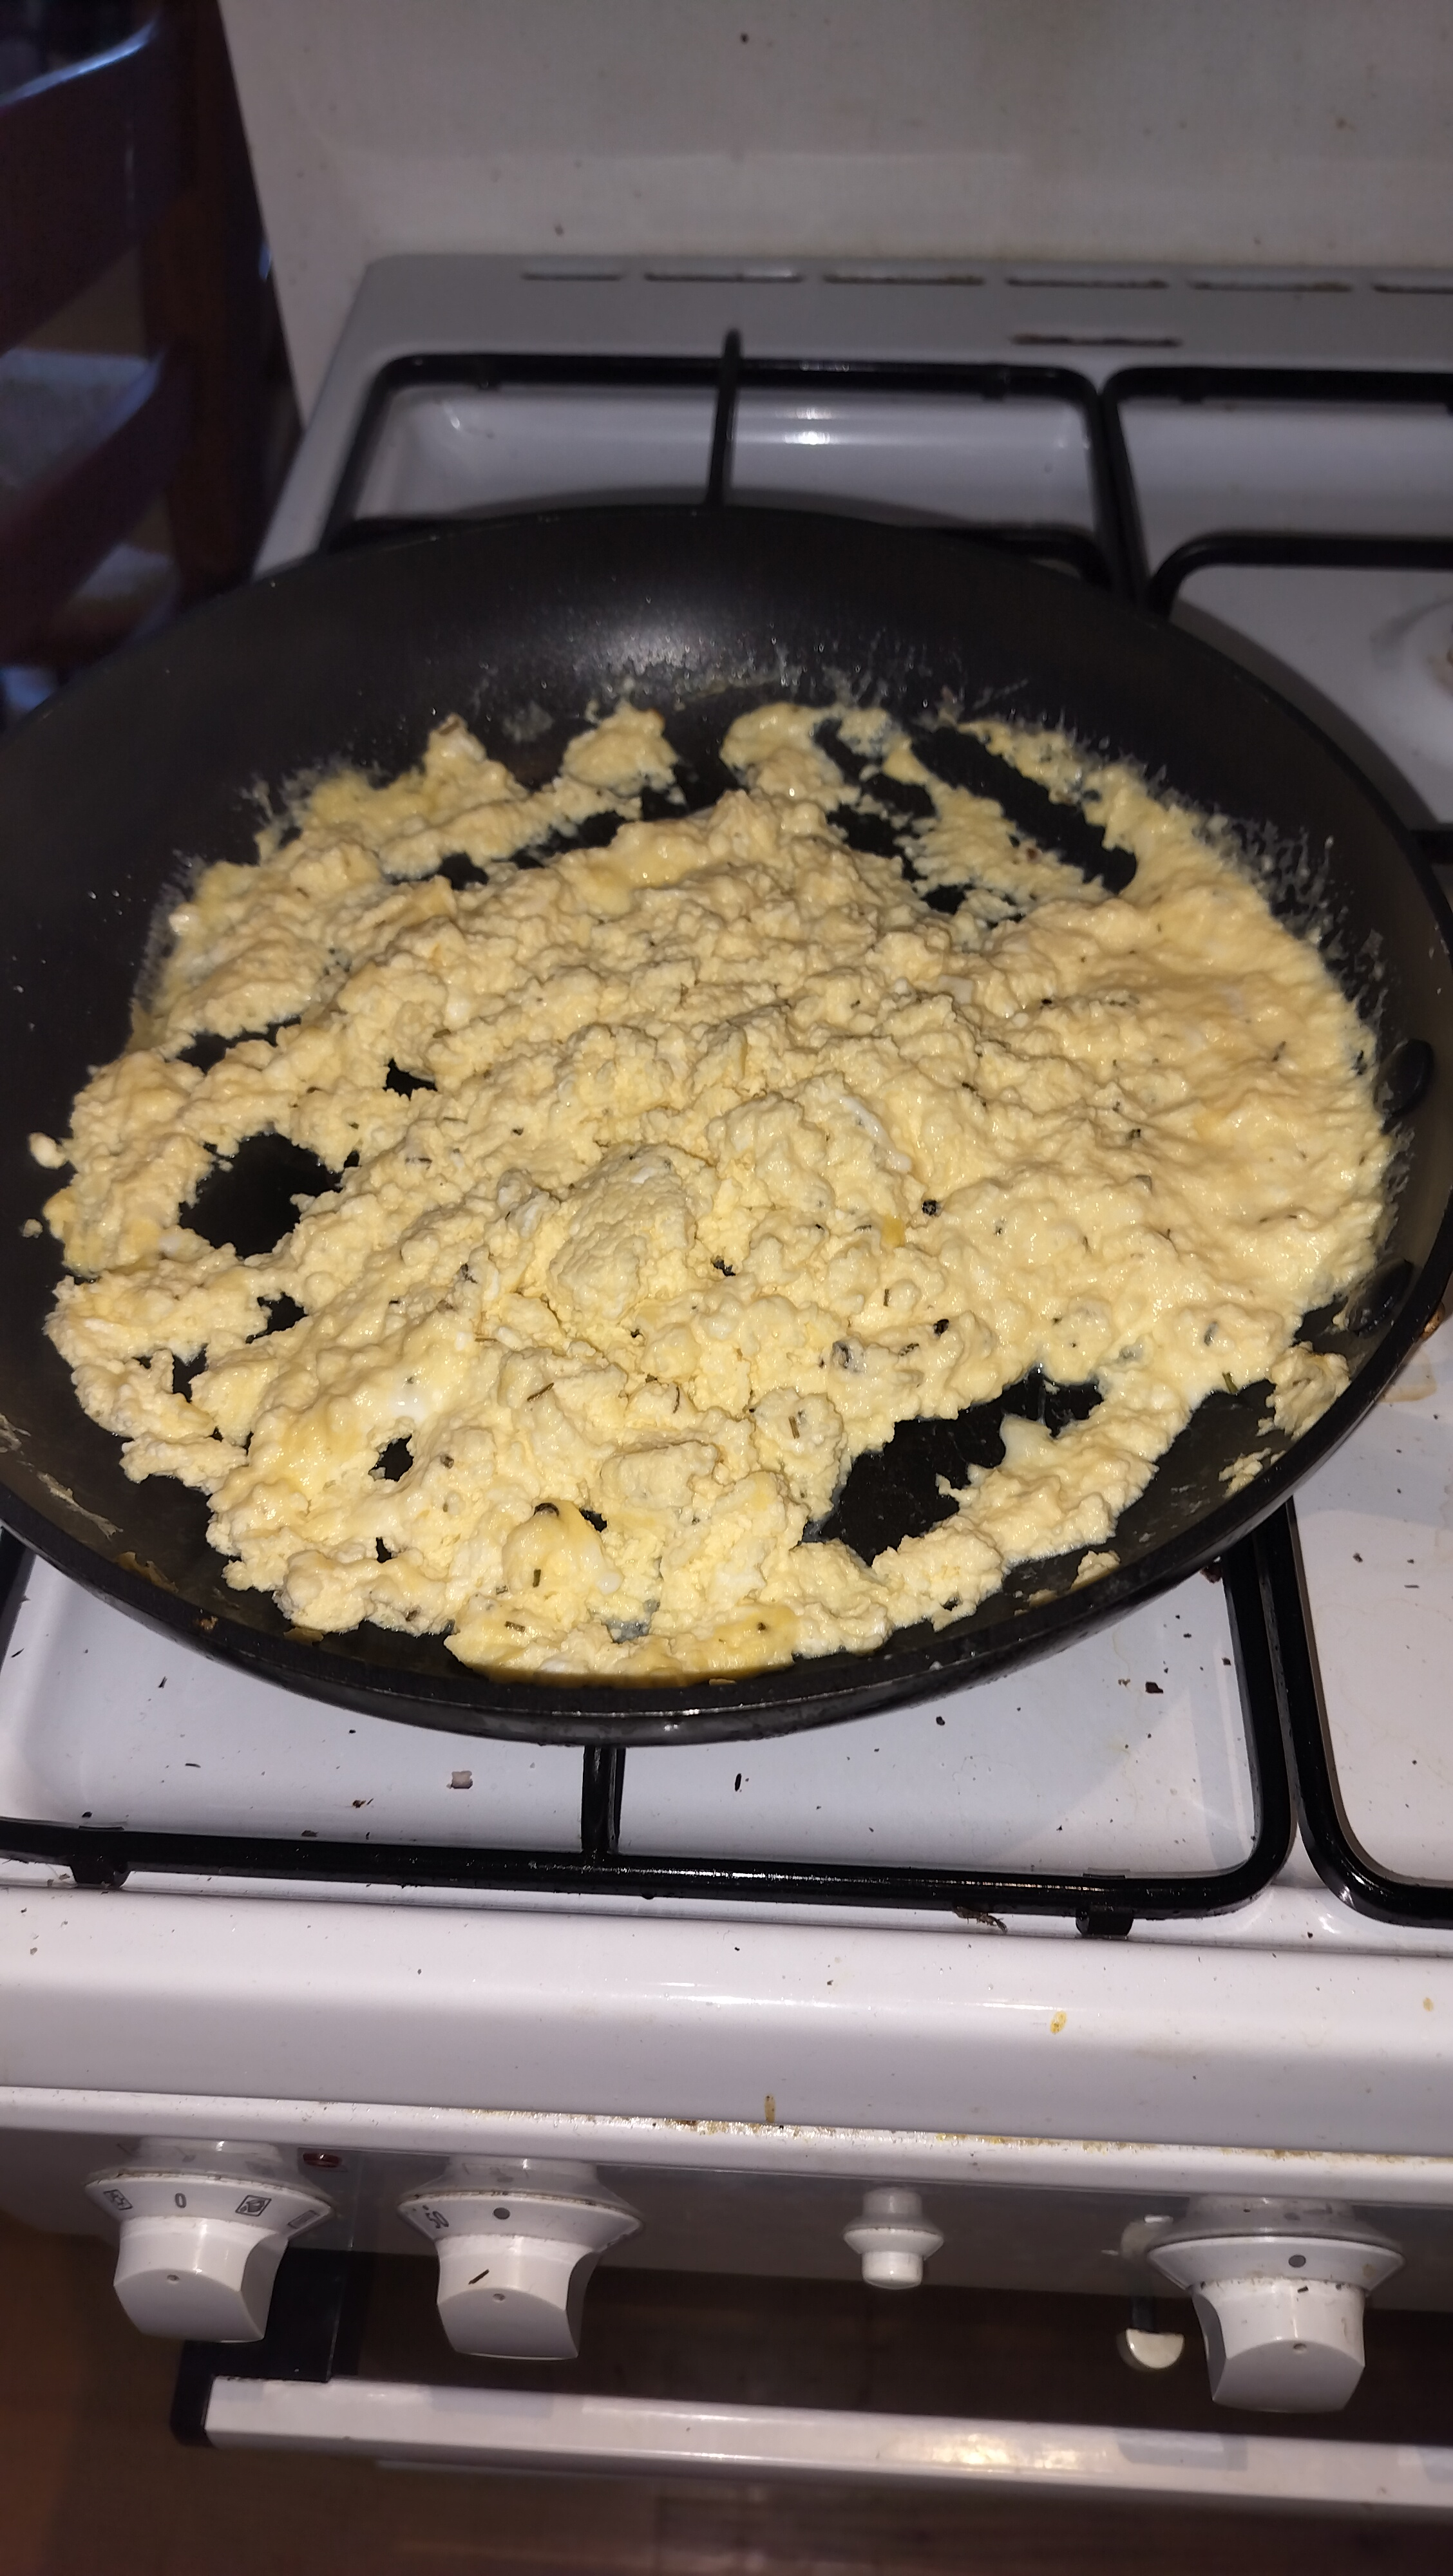
\includegraphics[width=\paperwidth,height=\paperheight]{Billeder/Morgenmad/Røræg.jpg}
    };
\end{tikzpicture}

\chapter{Frokost}
\minitoc
\clearpage \section{Couscous salat}
\begin{minipage}[t]{0.5\textwidth}
\textbf{Ingredienser:}
\begin{itemize}
    \item 200g Tørret couscous
    \item 500 mL kogende vand
    \item Kryderier
    \begin{itemize}
        \item Cayennepeber
        \item Paprika
    \end{itemize}
    \item Grøntsager
    \begin{itemize}
        \item Squash i Tern
        \item Peberfrugt
        \item Aubergine
        \item Tomatter
        \item Korainder
    \end{itemize}
\end{itemize}
\end{minipage}
\begin{minipage}[t]{0.5\textwidth}
\textbf{Fremgangsmåde:}
\begin{enumerate}
    \item Bland den tørret couscous med de ønskede krydderier. 
    \item Held det kogende vand på couscoussen i en plastik skål og lad det trække, der kan med fordel tilføjes mere vand hvis man ønsker en mere "våd" salat.
    \item Tilsæt til sidst grøntsagerne og server eventuel med hummus.
\end{enumerate}
\end{minipage}
\newpage
\begin{tikzpicture}[remember picture,overlay,inner sep=0pt,outer sep=0pt]
    \node[anchor=south east] at (current page.south east) {
        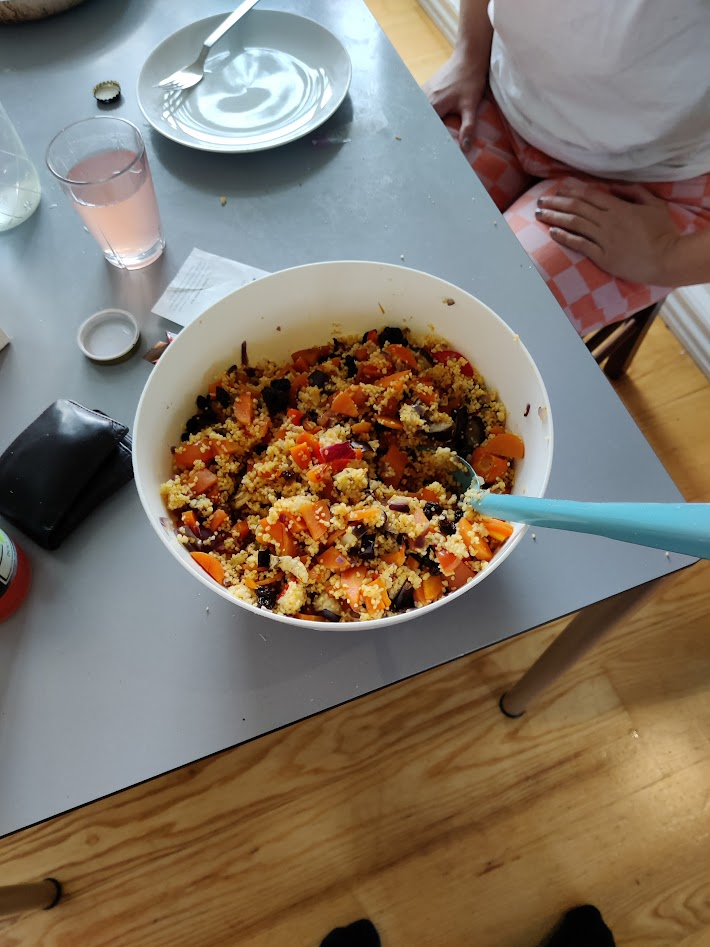
\includegraphics[width=\paperwidth,height=\paperheight]{Billeder/Frokost/Couscous.jpg}
    };
\end{tikzpicture}
\newpage \section{Tun mousse}
\begin{minipage}[t]{0.5\textwidth}
\textbf{Ingredienser:}
\begin{itemize}
    \item 3 dåse tun 
    \item 200g blødt smør
    \item 1 dL creme fraice
    \item Citronsaft
    \item Salt og pebber
\end{itemize}
\end{minipage}
\begin{minipage}[t]{0.5\textwidth}
\textbf{Fremgangsmåde:}
\begin{enumerate}
    \item Blød smøren
    \item Hæld vandet fra tunen, og "riv" tunen fra hianden til små stykker.
    \item Bland ingredienserne sammen til en blandet masse, og lad stå på køl, helst omkring 6 timer
\end{enumerate}
\end{minipage}
Jeg fortetrækker personligt tun i vand, men man kan sikker også bruge tun i olie.

\newpage Her mangler jeg igen et passende billede, så her er et billede af mig klædt ud som en havfrue\begin{figure}
    \centering
    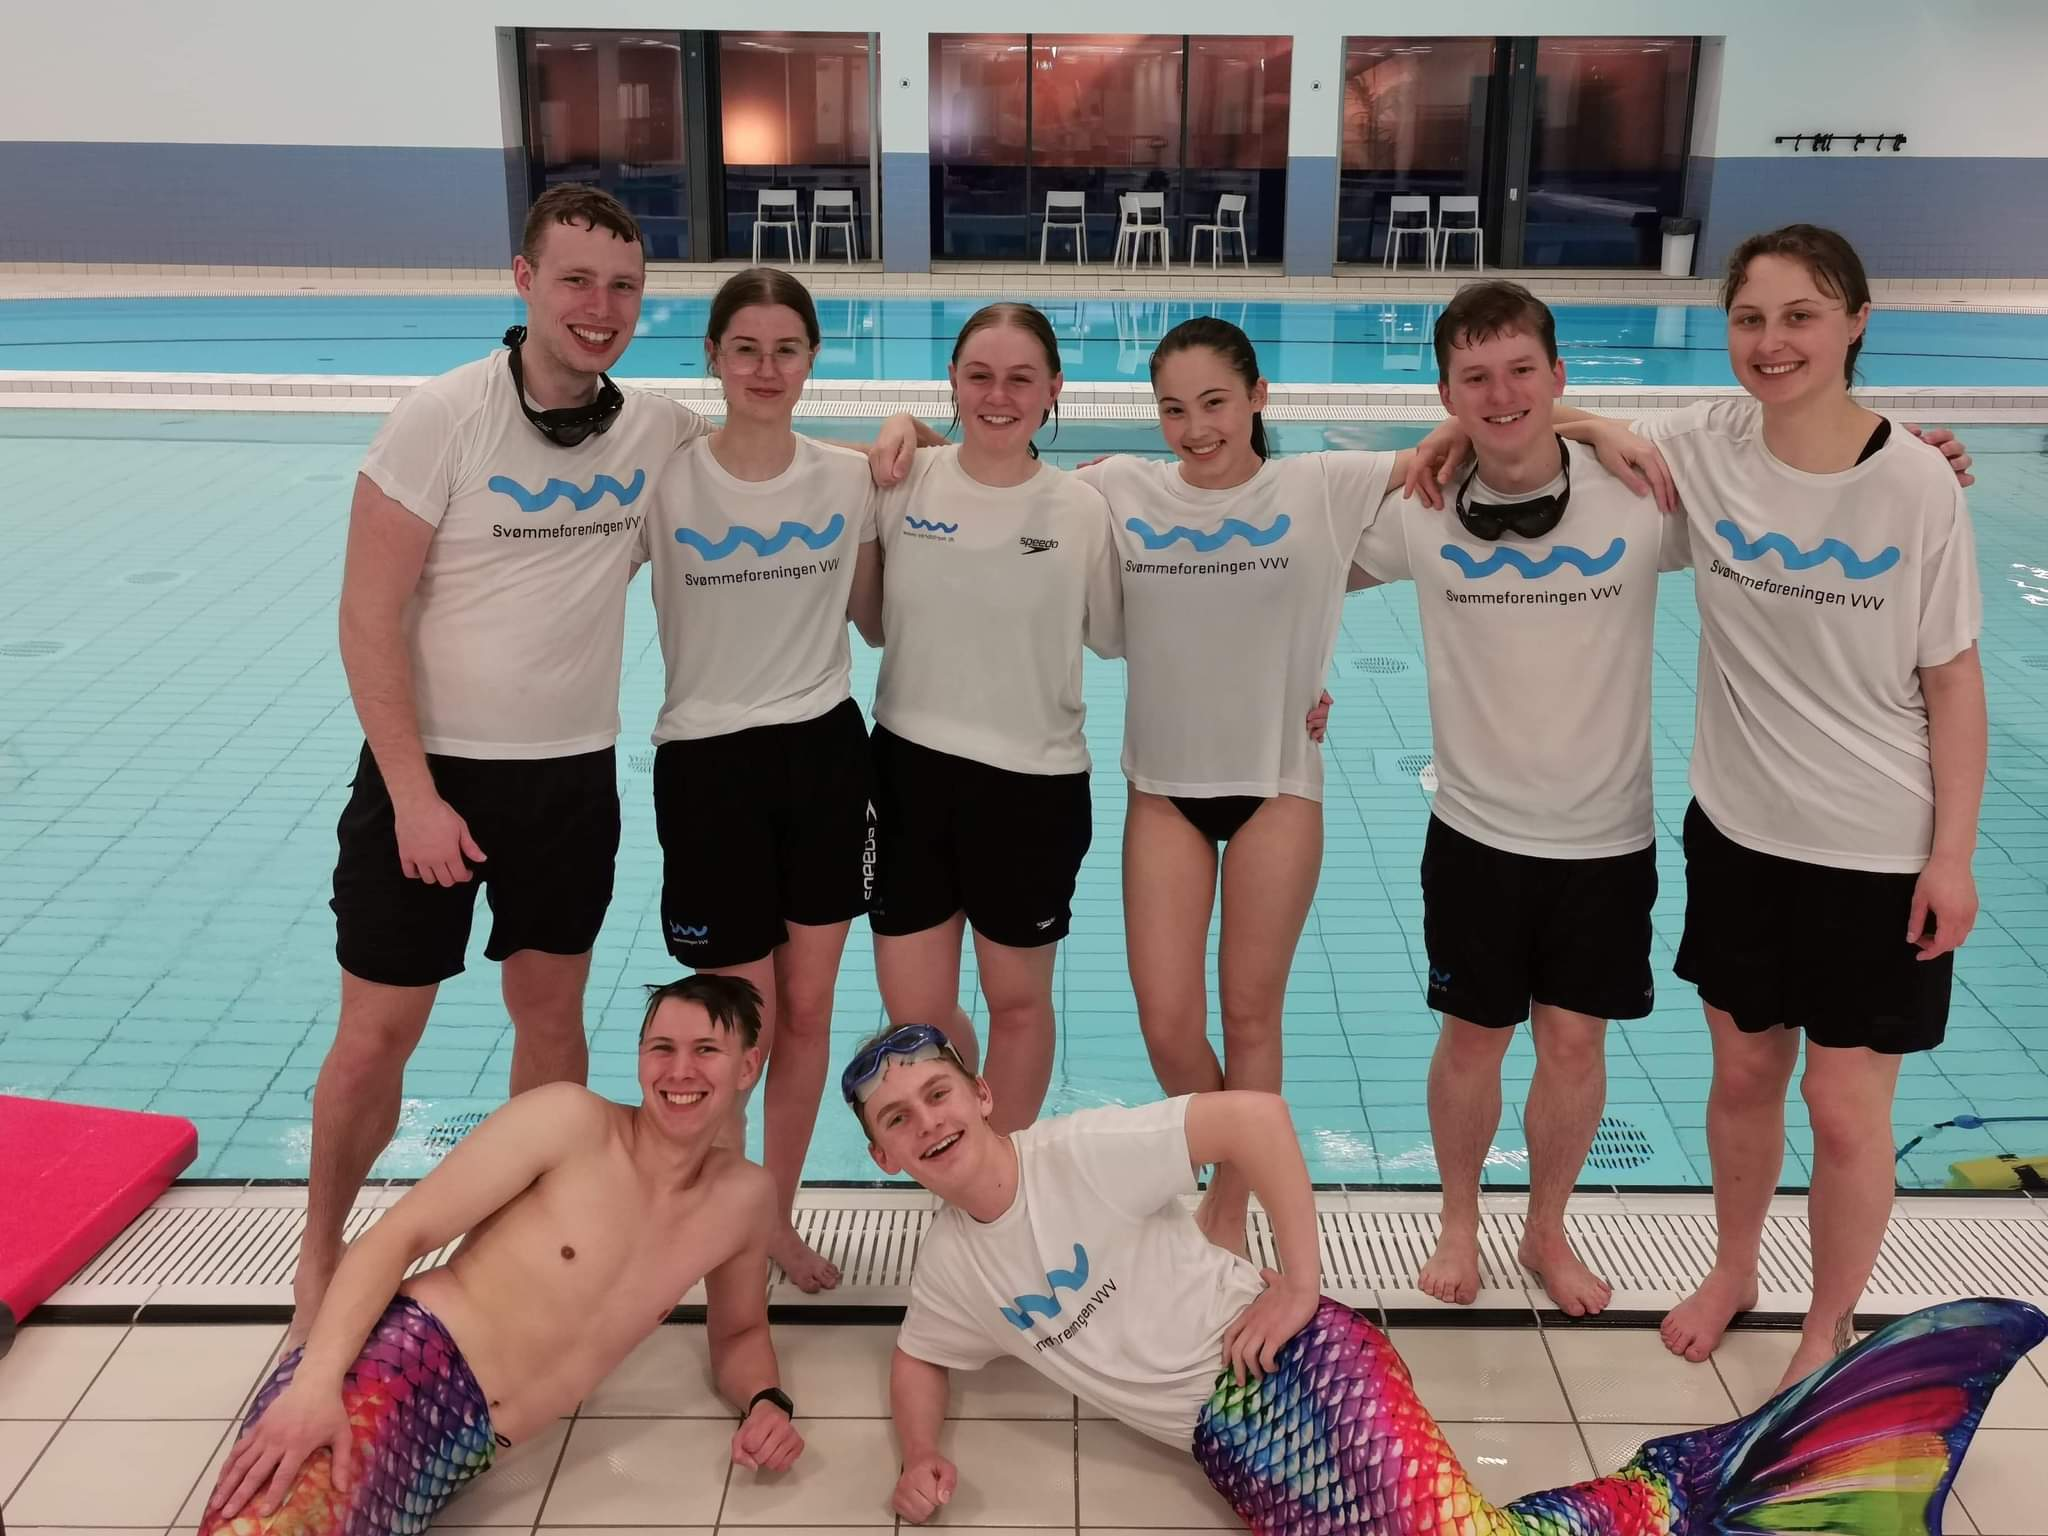
\includegraphics[width=0.75\linewidth]{received_483340176906259.jpeg}
    \caption{VVV coverbillede}
    
\end{figure}
\newpage \section{Vintersalat}
\begin{minipage}[t]{0.5\textwidth}
\textbf{Ingredienser:}
\\ Salaten: 
\begin{itemize}
    \item 150 g belugalinser
    \item 0.25 rødkål, fintsnittet
    \item 1 fennikel, fintsnittet
    \item 1 rødløg, i både
    \item 2 æble (mellemstore), i små tern
    evt.
    \begin{itemize}
        \item 1 tsk fennikel frø
        \item 1 appelsin, skåret i tern
    \end{itemize}
\end{itemize}
Dressing:
\begin{itemize}
    \item 1 spsk honning
    \item 2 spsk æblecidereddike
    \item 1 tsk dijon sennep
    \item 4 spsk olivenolie
\end{itemize}
\end{minipage}
\begin{minipage}[t]{0.5\textwidth} 
\textbf{Fremgangsmåde:}
\\ Salaten:
\begin{enumerate}
    \item Kog beluggalinserne jævnfør posens henvisning
    \item Lad linserne køle af, mens resten af ingredienserne klar gøres.
    \item Bland alle ingredienserne undtagen lidt af æblerne sammen med dressingen.
    \item Drys til sidst resten af æblerne oven på.
\end{enumerate}
Dressingen:
\begin{enumerate}
    \item Bland alle ingredienserne sammen og rør til ensartet konsistens.
    \item Gem lidt af dressingen til serveringen
\end{enumerate}
\end{minipage}
Hvis der ønskes en mere bitter version, kan man eventuelt tilføje mere dijon sennep.
\newpage  Her skulle der jo helst være et billede af en vintersalt, istedet for er der et billede af en måges fødder i Oslo, vinter 2018
\begin{figure}
    \centering
    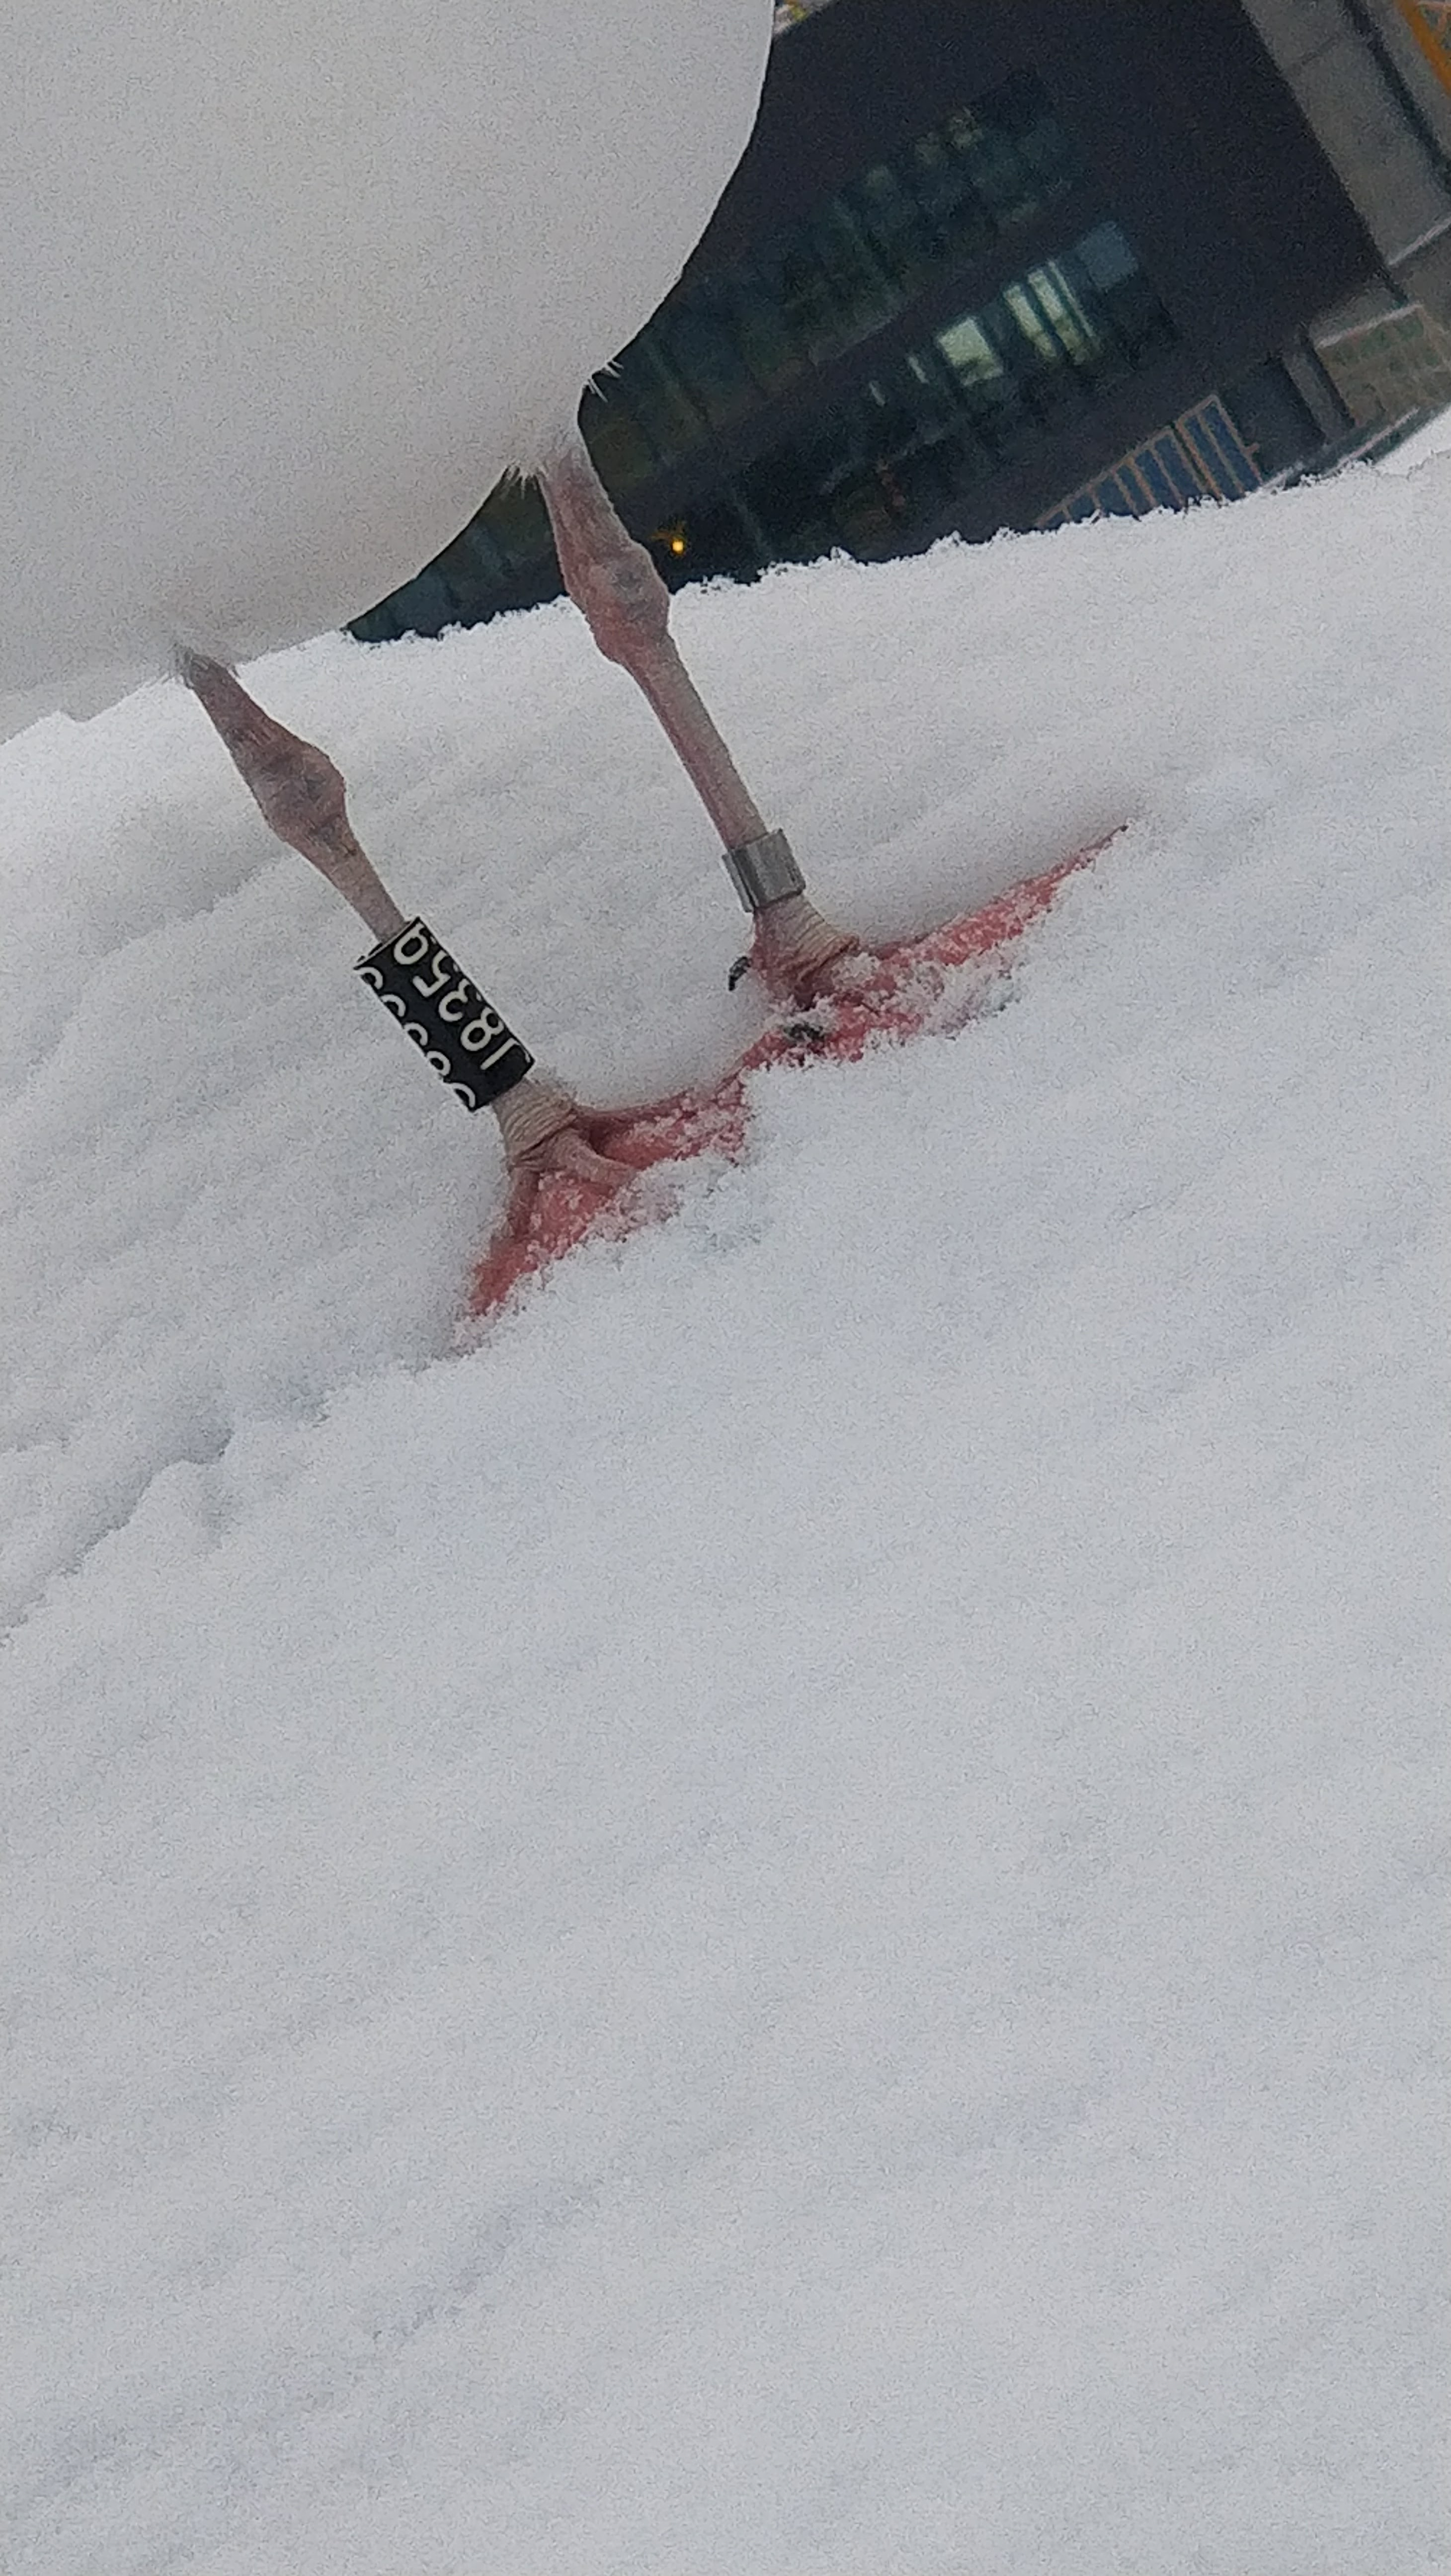
\includegraphics[width=0.5\linewidth]{Måge.jpg}
    \caption{Måge}
    
\end{figure}
\chapter{Ikke Vegetarisk Aftensmad} 
\minitoc
\newpage \section{Andebryststeg}
\begin{minipage}[t]{0.48\textwidth}
\textbf{Ingredienser:}
\begin{itemize}
    \item Optøet andebryststeg (700g)
    \item 25 g smør, blødgjort
    \item Timian
    \item Salt og peber
    \item Rodfrugter (evt øgo rodfrugt mix fra netto)
    \item 2 løg, skåret i både
\end{itemize}
\end{minipage}
\begin{minipage}[t]{0.48\textwidth}
\textbf{Fremgangsmåde:}
\begin{enumerate}
    \item Gnid skindet med en blanding af, blødgjort smør, timian, salt og peber.
    \item Lig anden i et ovnfast fad, med løg og rodfrugter rundt om
    \item Steg anden i forvarmet ovn på 200 \degree C varmluft i 40-45 minutter
    \item Sæt ovnen på grill og skru op på 250 \degree C for at give et sprødt skind, omtrent 5 minutter.
\end{enumerate}
\end{minipage}
\textcolor{white}{Herkujkdansdaskdaskjdhsaidgasdhasiuhdashdbasjkdnasidhbsandusahdbjnashdjkashnidu\\ dsadjiasojdsaodjiasojdasi jdasiojdasioj iasdioas sadasoidas \\}
Efter endt stegning kan man med fordel bruge sovsen i fadet til en brun sovs. Efter min oplevelse er det 40-45 minutter der giver en let rød and, hvis det ønskes gennemstegt, kan man give den lidt mere. Server gerne anden med rodfrugterne eventuelt sammen med kartofler.
Har fundet denne oversigt på nettet over kernetemperatur for and:

\begin{table}[b]
    \centering
    \begin{tabular}{c|c}
         Farve & Kerne temperatur  \\ \hline
         \cellcolor{red!25} Rosa &  62-63 \degree C \\
         \cellcolor{red!35}Let Rosa & 64-65 \degree C   \\
         \cellcolor{brown!40}Gennemsteg & 70-72 \degree C   \\ 
    \end{tabular}
    \caption{Kernetemperatur for stegning af andebryststeg}
\end{table}
\newpage
\begin{tikzpicture}[remember picture,overlay,inner sep=0pt,outer sep=0pt]
    \node[anchor=south east] at (current page.south east) {
        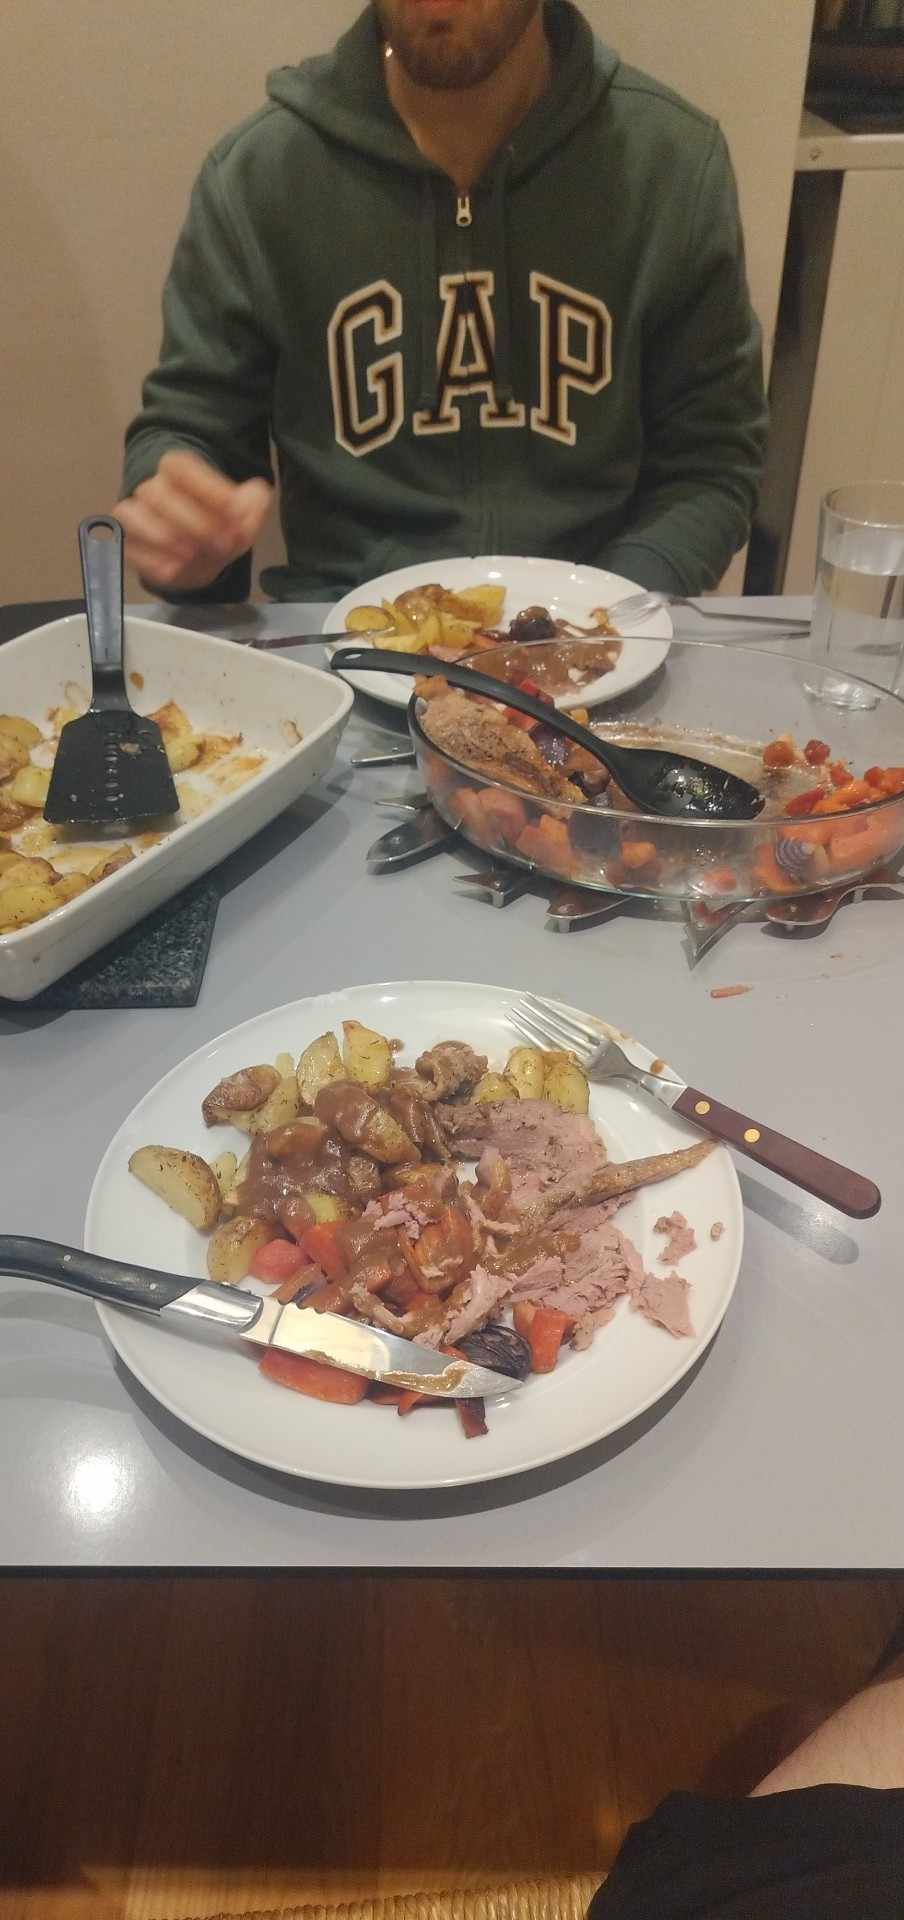
\includegraphics[width=\paperwidth,height=\paperheight]{Billeder/Aftensmad/Andebryststeg.jpeg}
    };
\end{tikzpicture}
\newpage \section{Butter Chicken}
\begin{minipage}[t]{0.5\textwidth}
\textbf{Ingredienser:}
\begin{itemize}
    \item 1-2 Løg
    \item 1/2 dL piskefløde
    \item 50g smør
    \item 2spsk olivenolie
    \item 500 g kylling skåret i tynde stykker, kyllingbrust, inderfillet eller ligende
    \item salt og pebber
    \item Marinade
    \begin{itemize}
        \item 1 dåse hakkede tomatter
        \item 100 g græsk yoghurt (18\%)
        \item 2 tsk chiliflager
        \item 2 tsk stødt spidskommen
        \item 1 tsk stødt kardemomme
        \item 2 tsk garam masala
        \item 2-3 fed hvidløg, presset
        \item 1-2 tsk stødt gurkemejer
        \item 1 tsk tørret ingefær
        \item Evt.
        \begin{itemize}
            \item 1/2 tsk Nellike
            \item 1 tsk Karry
            \item 1 spsk hakket, tørret chillier
        \end{itemize}
    
    \end{itemize}
\end{itemize}
\end{minipage}
\begin{minipage}[t]{0.5\textwidth}
\textbf{Fremgangsmåde:}
\begin{enumerate}
    \item Bland marinaden sammen til en ens masse, og put kylling i, lad stå i køleskabbet så længe som muligt.
    \item Skær løgene til ringe.
    \item Smelt smøren, og olien i en gryde og svits løgene til let gennemsigtige.
    \item Tilsæt kyllingen med den tilhørende sovs, samt fløden
    \item Bring det i kog, og lad simre i 30-35 minutter, til kyllingen stortset smuldre.
\end{enumerate}
\end{minipage}
Til butter chicken skal kylling marinerer stort set så længe som muligt, det bliver utroligt mørt hvis man kan give det 24 timer i køleskabet, men smagen er kommer også af kortere tid.
\newpage Her skulle der være et billede, har dog ikke kunne finde et så her er et billede af mig der klatre, indtil jeg laver retten igen.
\begin{figure}
    \centering
    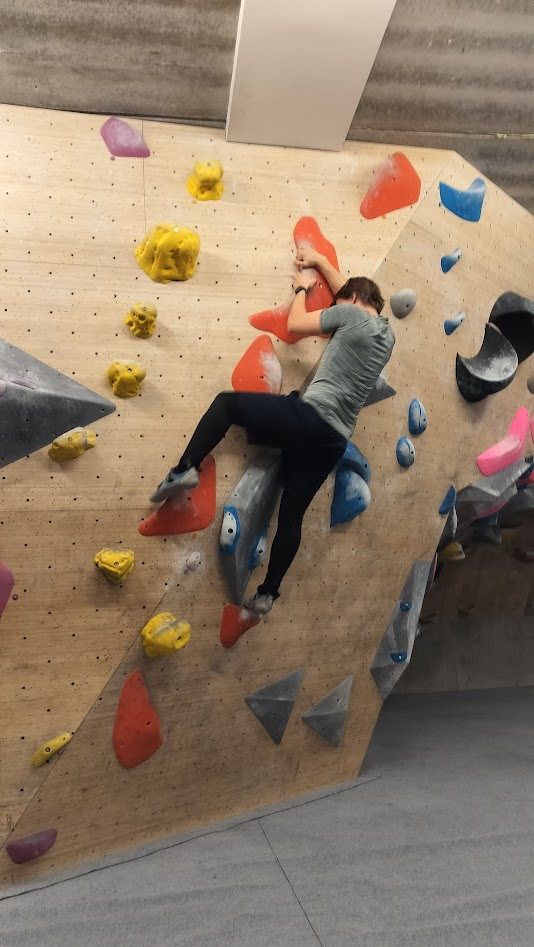
\includegraphics[width=0.5\linewidth]{Klatring.jpg}
    \caption{Mig dig klatre kort tid inden jeg fik svar fra python eksamen}
    \label{fig:Klatring}
\end{figure}
\newpage \section{Carbonarra}
\begin{minipage}[t]{0.5\textwidth}
\textbf{Ingredisner:}
\begin{itemize}
    \item 250 g pasta
    \item 100-150g bacon i tern
    \item 1 tsk smør
    \item 1-2 finthakket løg
    \item 1 dL piskefløde
    \item 2 æg
    \item 75g revet parmesan(eller ligende ost)
    \item Friskkværnet peber
\end{itemize}
\end{minipage}
\begin{minipage}[t]{0.5\textwidth}
\textbf{Fremgangsmåde:}
\begin{enumerate}
    \item Kog pastaen til ønskede konsistens, anbefaller al dente.
    \item Steg baconen, og sæt til siden.
    \item Smelt smøren i en gryde, og svits løgne til gyldne.
    \item Tilsæt bacon og fløde, og lad fløden kortvarigt bruse op .
    \item Skru ned for varmen/fjern fra pluset, og rør æggene samt pastaen i. 
    \item Tilsæt til sidst den revet ost.
\end{enumerate}
\end{minipage}
\newpage
Her mangler jeg igen et billede, så her er der throwback til sommer 2019 til telttur i Sverige.
\begin{figure}
    \centering
    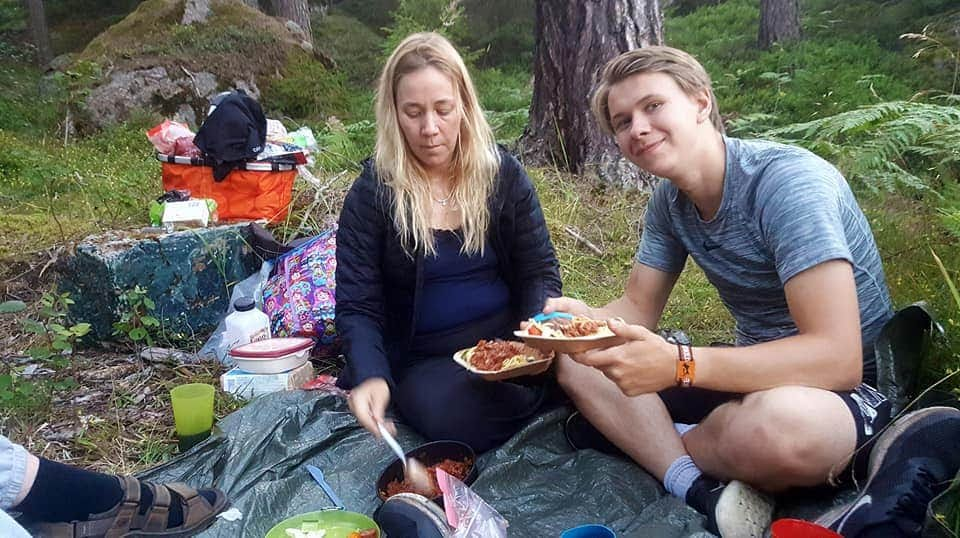
\includegraphics[width=0.5\linewidth]{Skovtur_Sverige.jpg}
    \caption{Mad i sverige}
    \label{fig:Arbitær 2}
\end{figure}
\newpage \section{Confit De Canard}
\begin{minipage}[t]{0.5\textwidth}
\textbf{Ingrediesner:} 
\begin{itemize}
    \item 2 andelår eller andebryst
    \item 2-3 lauerbærblade
    \item Timian
    \item Salt og peber
    \item 500 g andefedt (skal ikke bruges til Sous vide)
\end{itemize}
\end{minipage}
\begin{minipage}[t]{0.5\textwidth}
\textbf{Fremgangsmåde:}
\\ I gryde 
\begin{enumerate}
    \item Gnid anden med timian, salt og peber, og lad marinere natten over i køleskab.
    \item Smelt andefedtet i en gryde, i et lag hvor anden kan helt druknes i fedtet (fedtet skal helst varmes til omtrent 100 \degree C).
    \item Lig anden forsigtigt i, og tilsæt lauerbærbladene. 
    \item Kog i mindst 2 timer til kødet er meget mørt (det skal helst rives i stykker med en gaffel).
    \item Når de er godt møre steg anden på panden ved høj varme til at give et crispy finish til skindet.
\end{enumerate}
Sous vide
\begin{enumerate}
    \item Til sous vide er trinene det samme, men frem for at marinere natten over og stege i en gryde, skal den blot have 24-36 timer i sous vide.
    \item Steg også her på panden ved høj varme. 
\end{enumerate}
\end{minipage}
Har endnu ikke kastet mig ud i at sous vide andelår/andebryst, men tænker også det kunne tilføje noget til smagen hvis man i vakumposen tilsætte lidt andefedt, såleddes det steges i dets eget fedt.
%\newpage \begin{tikzpicture}[remember picture,overlay,inner sep=0pt,outer sep=0pt]
%    \node[anchor=south east] at (current page.south east) {
%        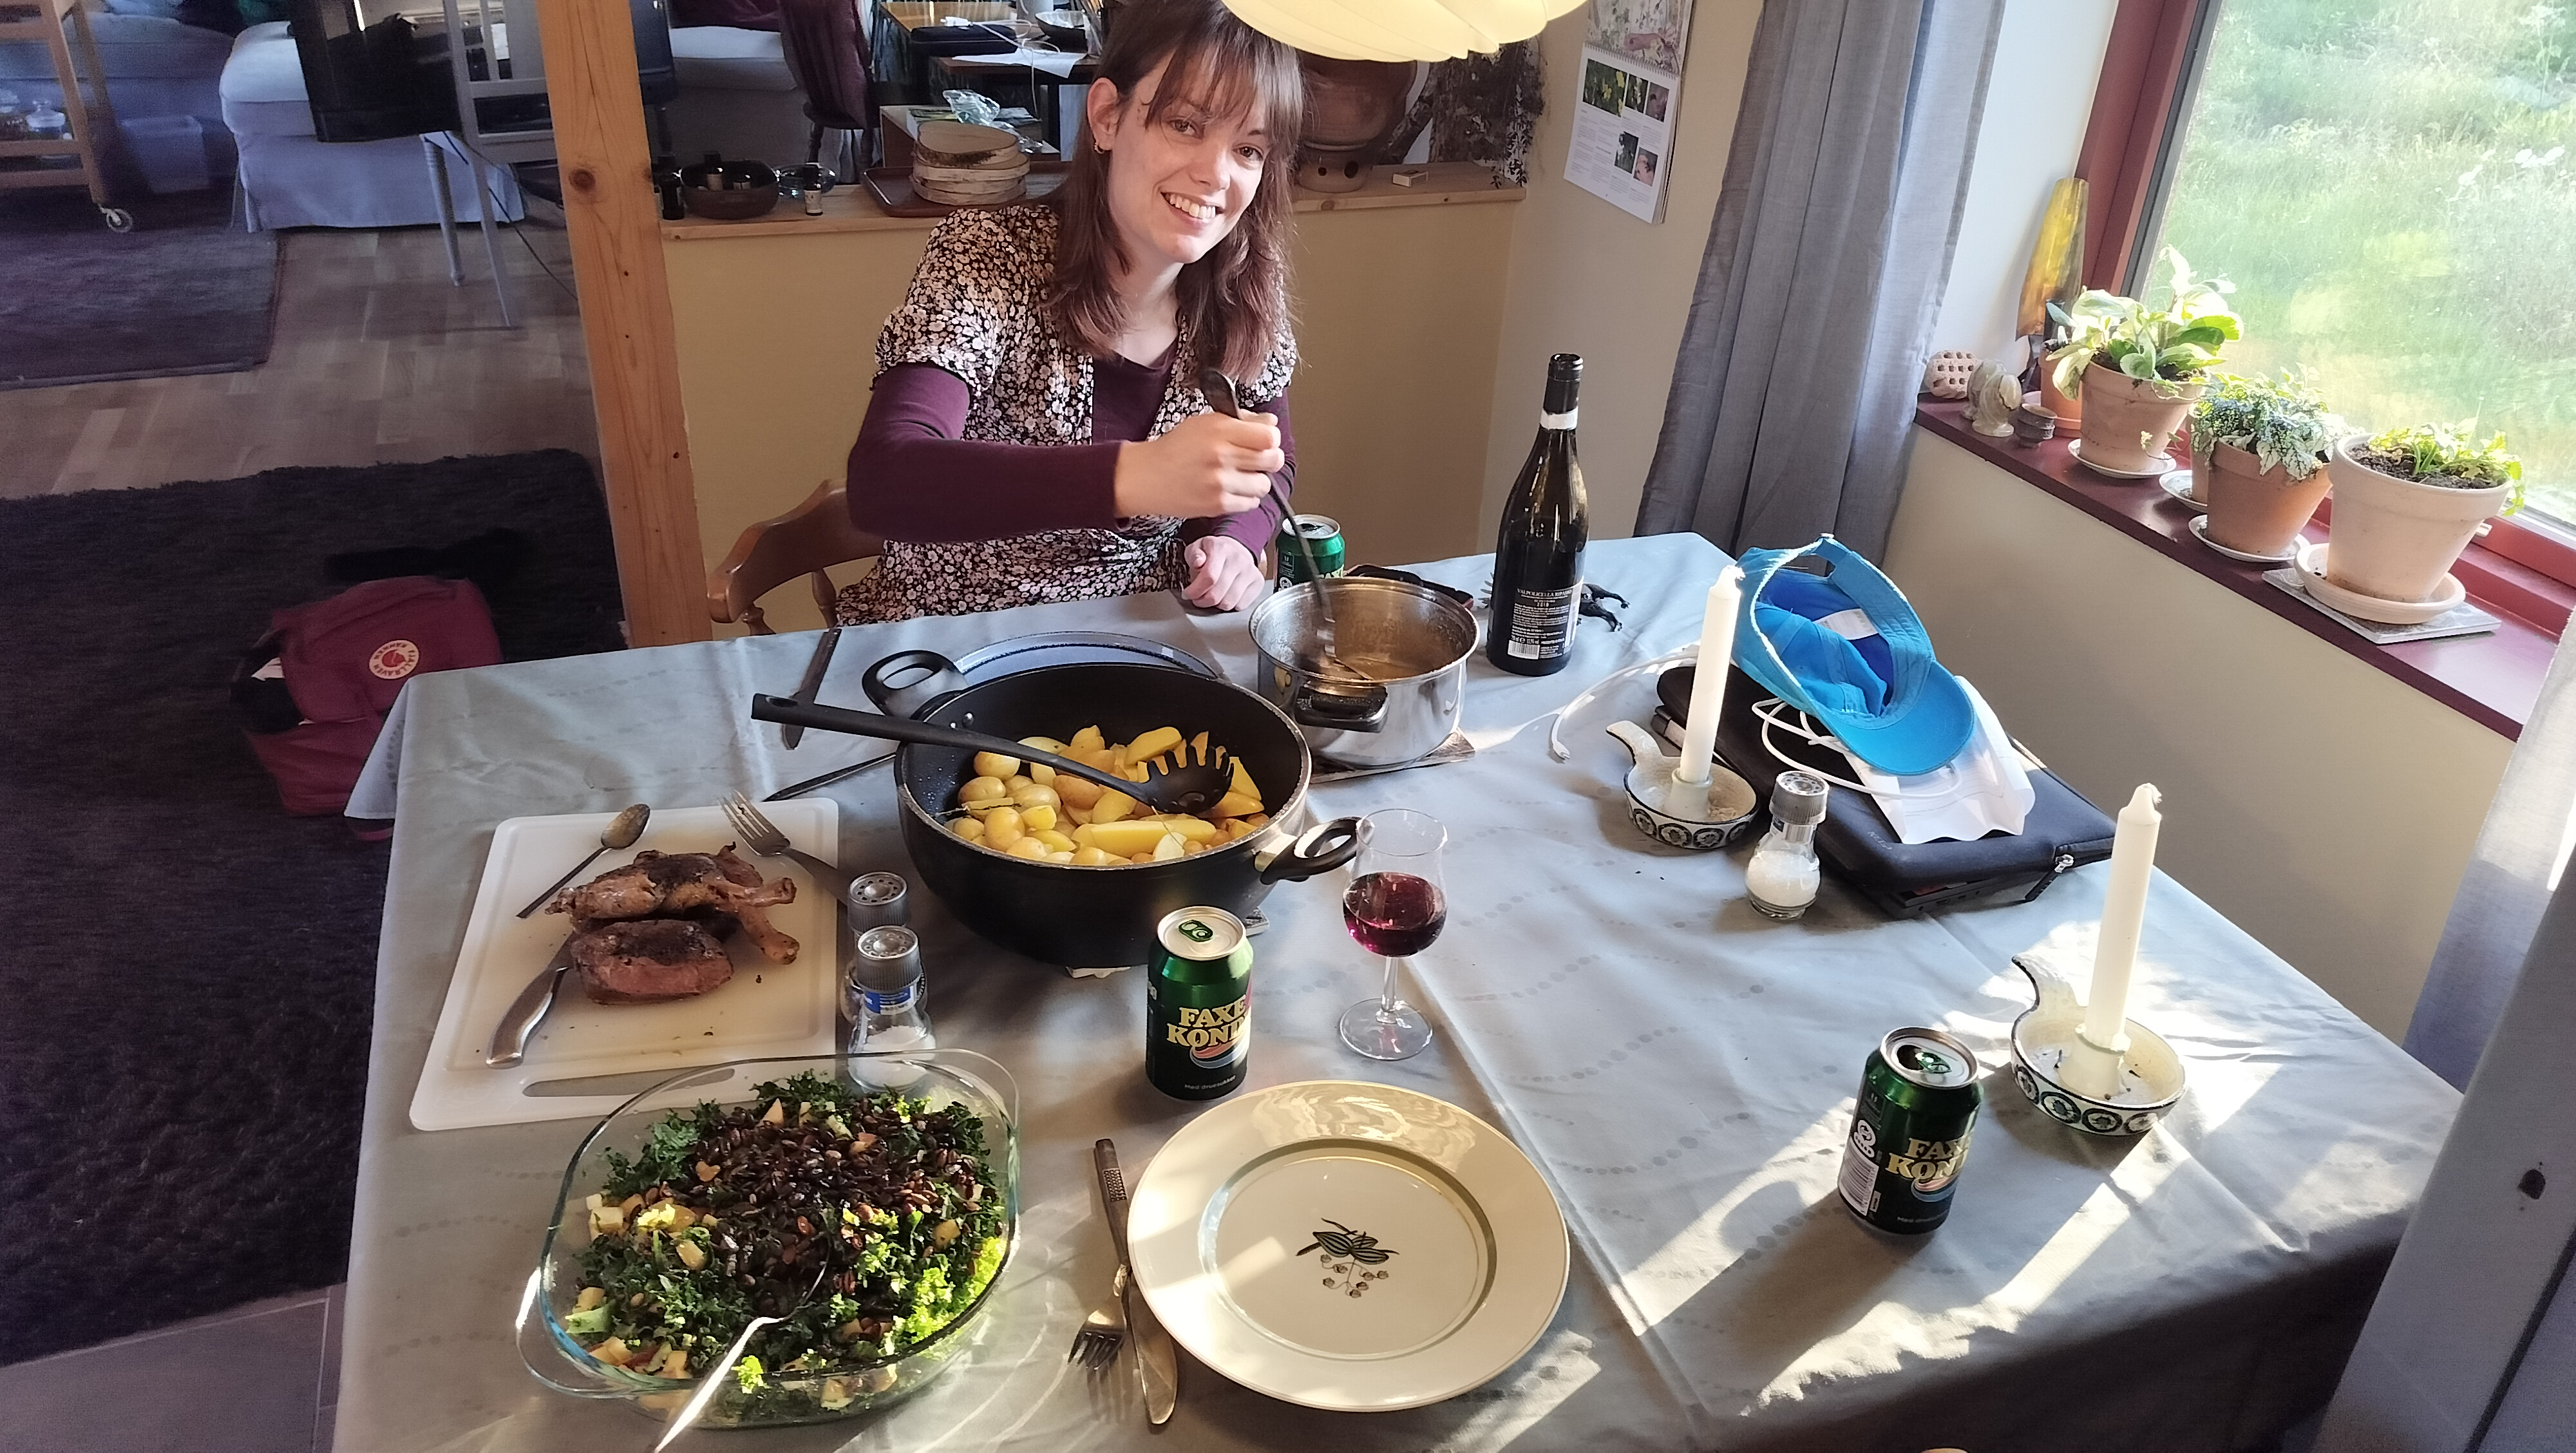
\includegraphics[width=\paperwidth,height=\paperheight]{Billeder/Aftensmad/Confit_De_Canard.jpg}
%    };
%\end{tikzpicture}
\newpage \begin{tikzpicture}[remember picture,overlay,inner sep=0pt,outer sep=0pt]
    \node[anchor=south east] at (current page.south east) {
        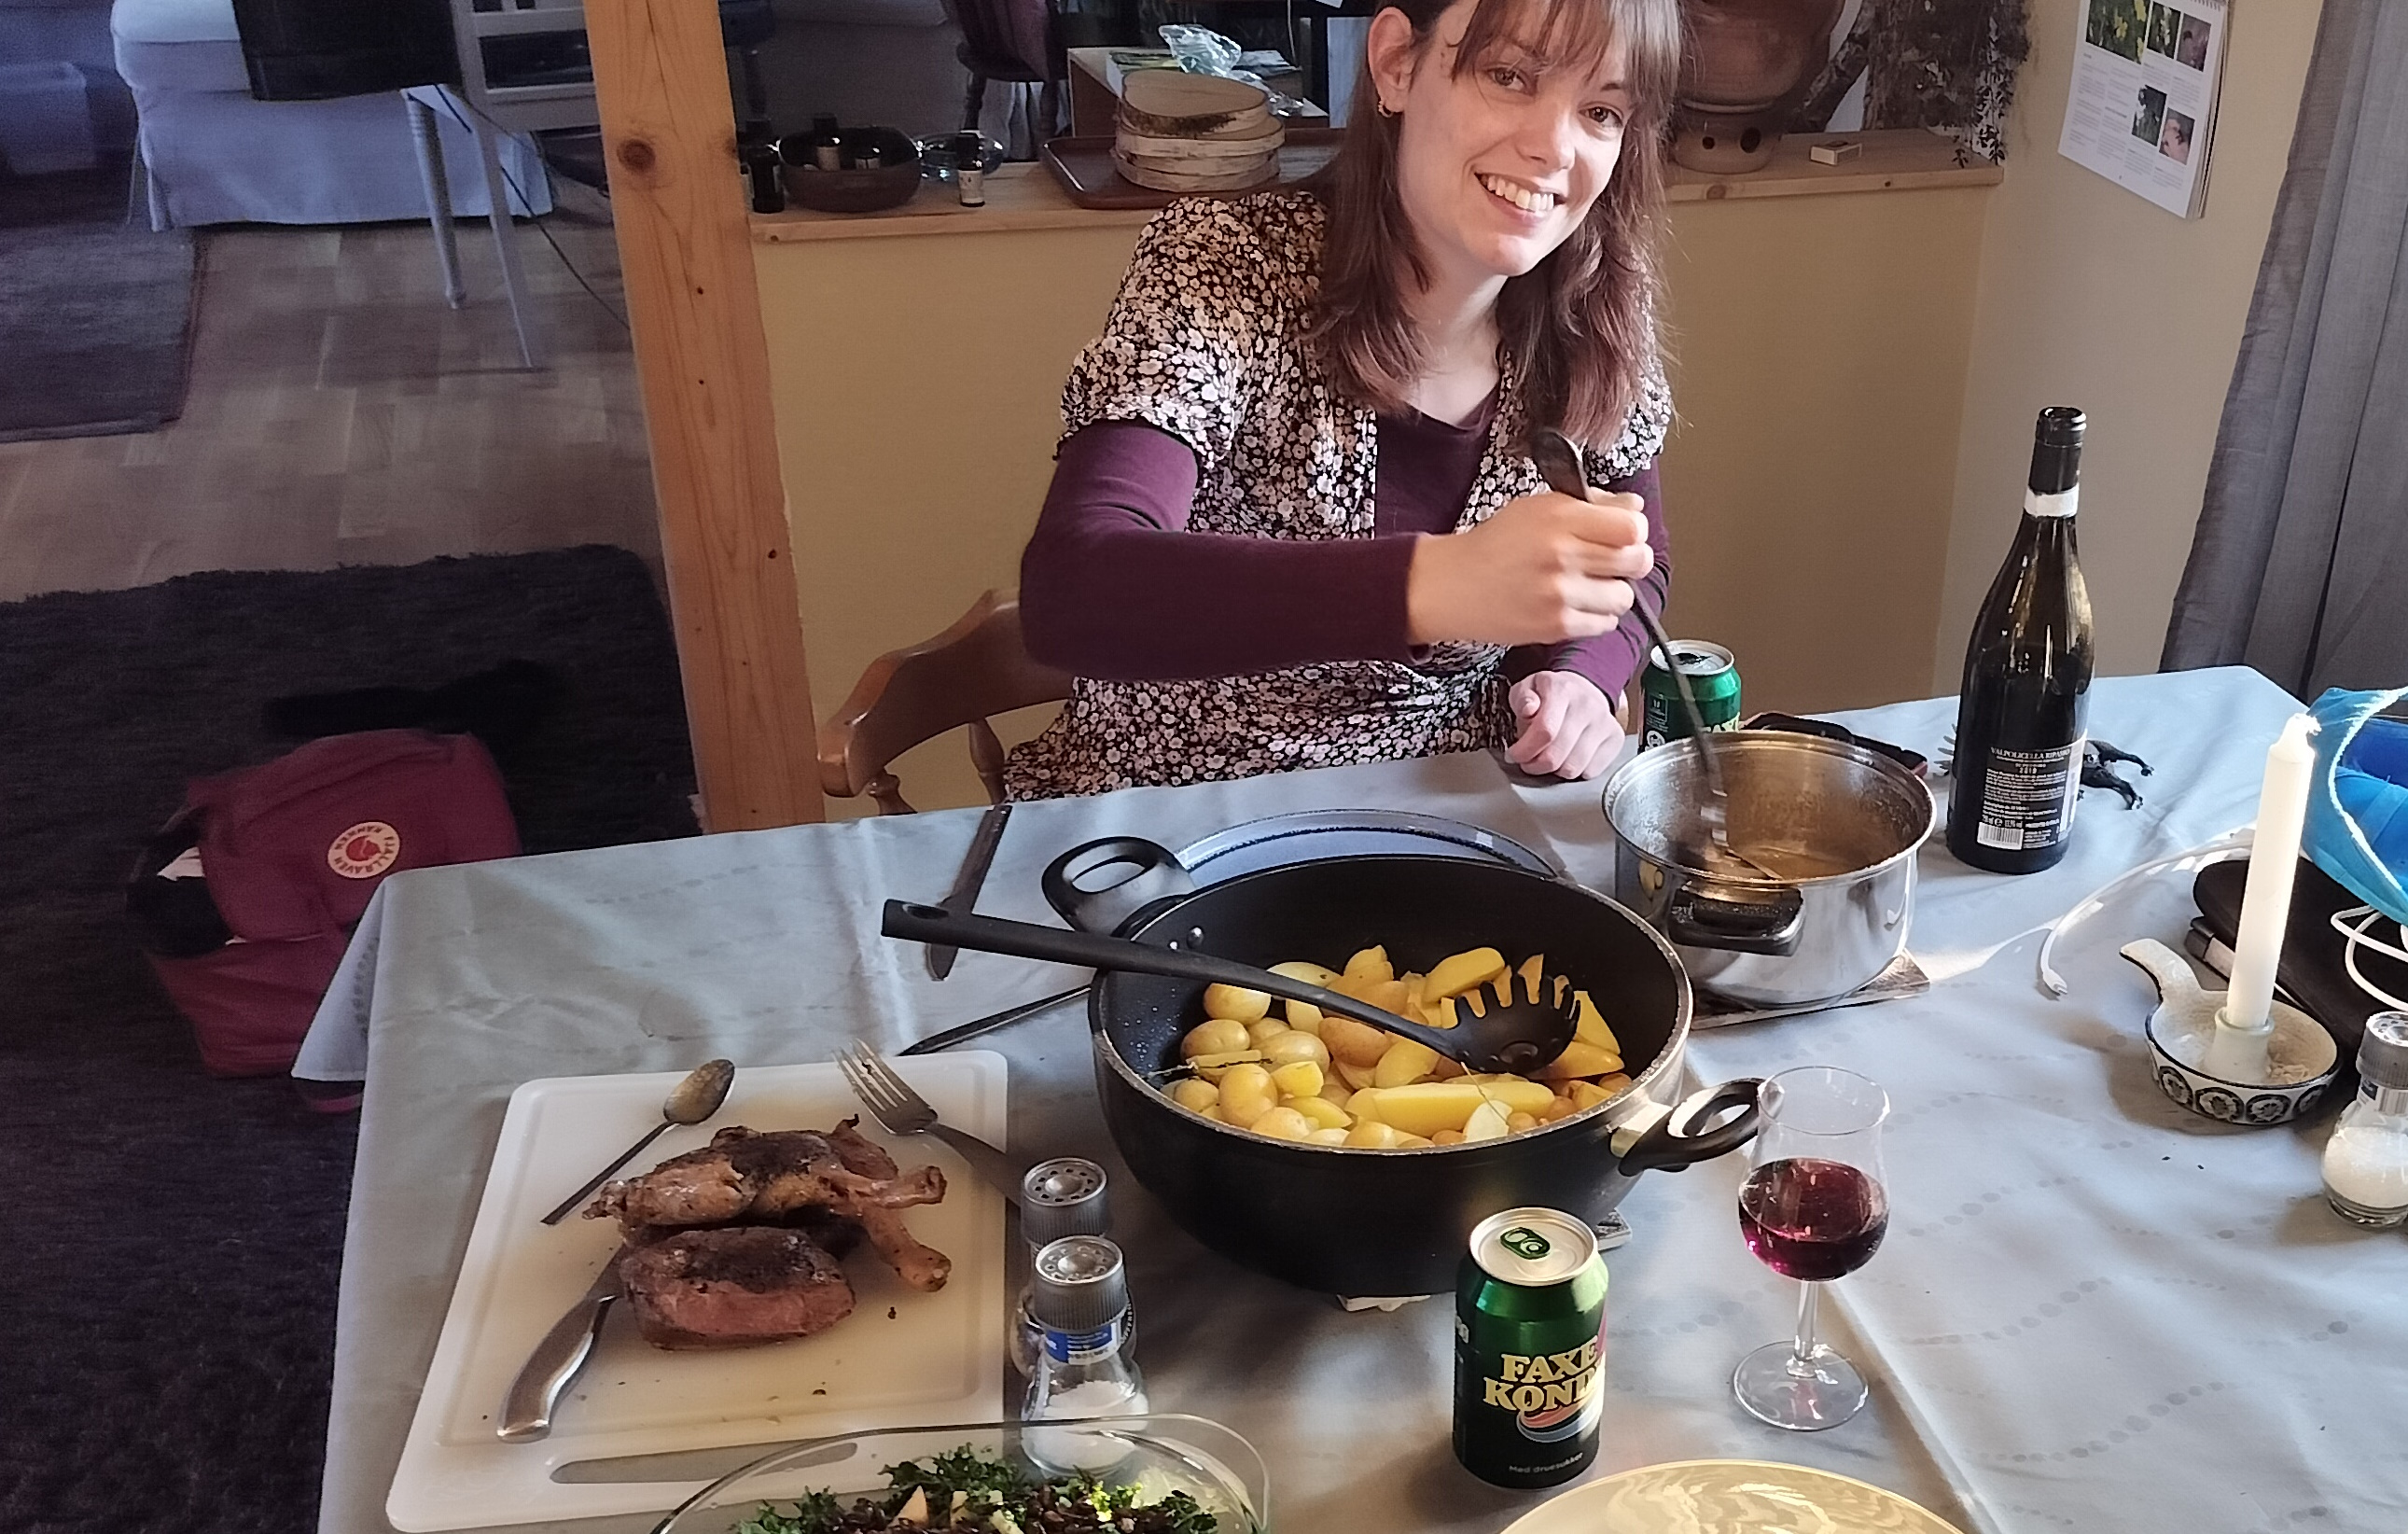
\includegraphics[width=\paperwidth,height=\paperheight]{Billeder/Aftensmad/Confit 2.jpg}
    };
\end{tikzpicture}
%\newpage Her mangler jeg desværre også et billede, så her kommer der et billede fra BRSS åben hus 
%\begin{figure}
%    \centering
%    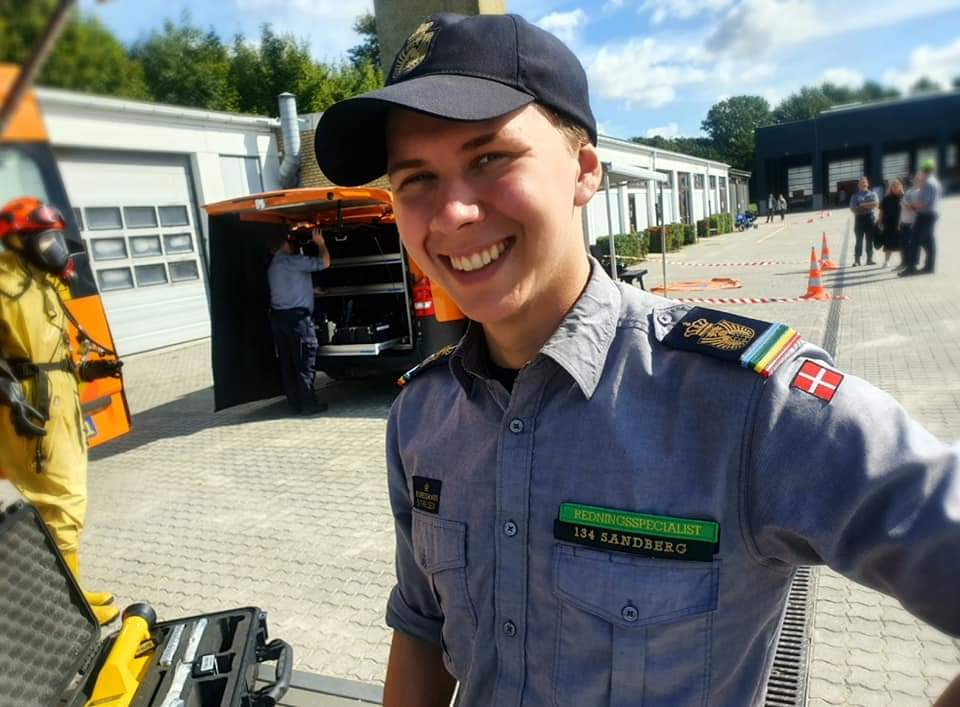
\includegraphics[width=0.5\linewidth]{BRSS.jpg}
%    \caption{Åben Hus Beredskabsstyrelsen Sjælland}
%\end{figure}
\newpage \section{Flæskesteg}
\begin{minipage}[t]{0.5\textwidth}
\textbf{Ingredienser}
\begin{itemize}
    \item Flæsesteg, helst med en tyk fedram
    \item Flagesalt eller groft salt
    \item Lauerbærblade (cirka 1 per 2-3 sværd)
    \item En smule timian
\end{itemize}
\end{minipage}
\begin{minipage}[t]{0.5\textwidth}
\textbf{Fremgangsmåde:}
\begin{itemize}
    \item Rids sværne dybe, til så dybt som muligt, der må ikke ridses ned i selve kødet.
    \item Gnid flæskstengen med krydderierne og fordel lauerbærbladene
    \item Put i ovnen på en rist ovenover en brædepande fyldt med vand og tænd op 175 \degree C. 
    \item Steg til 60 \degree C i midten
    \item Hvis ikke sværdene er blevet så sprøde som forventet kan man afslutte med 250 \degree C grill
\end{itemize}
\end{minipage}
\newpage  \begin{tikzpicture}[remember picture,overlay,inner sep=0pt,outer sep=0pt]
    \node[anchor=south east] at (current page.south east) {
        \includegraphics[width=\paperwidth,height=\paperheight]{Billeder/Aftensmad/Flæskesteg.jpg}
    };
\end{tikzpicture}
\newpage \section{Fruta de Mer}
\begin{minipage}[t]{0.5\textwidth}
\textbf{Ingredienser:}
\begin{itemize}
    \item 250g Pasta(jeg fortrækker en form for linguinne)
    \item 250g arabiatta sauce (Variende alt efter hvor tomattet den skal være)
    \item Skaldyr(rejer,blåmuslinger og hvad man ellers lige har lyst til)
    \begin{enumerate}
        \item Rejer (evt firske vanamamme rejer)
        \item 500 g Blåmuslinger
        \item Evt. Krabbe
        \item Evt. laks
    \end{enumerate}
    \item Persille og citron til servering
\end{itemize}
\end{minipage}
\begin{minipage}[t]{0.5\textwidth}
\textbf{Fremgangsmåde:}
\begin{enumerate}
    \item Kog pastaen til al dente og sæt til siden.
    \item Klargør de forskellige skaldyr (se eventuel opskrift på Moulles-firtes).
    \item Tilsæt arabiatta saucen til den kogte pasta, og fold ind.
    \item Tilsæt skaldyren og rør rundt til det er ligelidt fordelt.
    \item Server med persille og citronsaft.
\end{enumerate}
\end{minipage}
\newpage
\begin{tikzpicture}[remember picture,overlay,inner sep=0pt,outer sep=0pt]
    \node[anchor=south east] at (current page.south east) {
        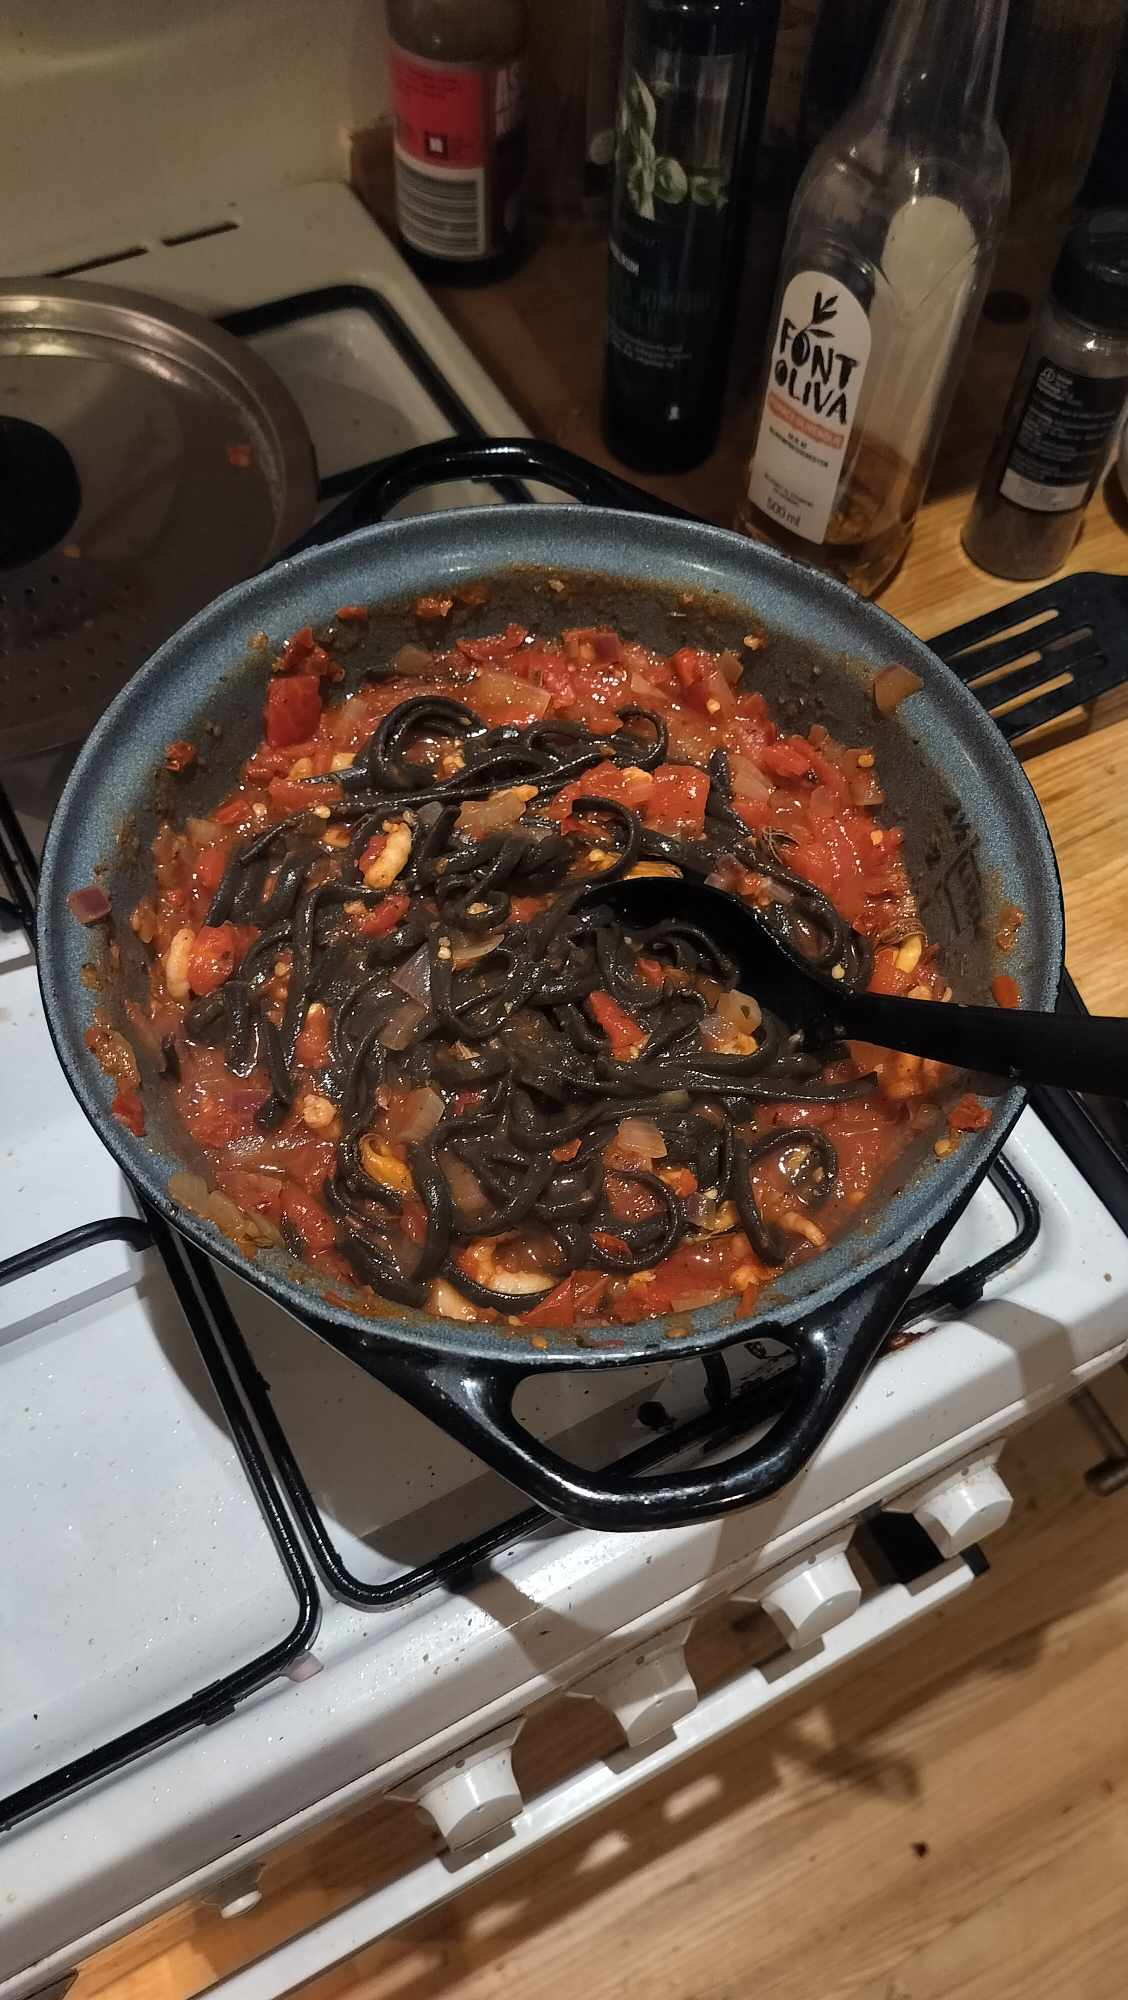
\includegraphics[width=\paperwidth,height=\paperheight]{Billeder/Aftensmad/Fruta_de_mer.jpg}
    };
\end{tikzpicture}
\newpage \section{Laksepasta}
\begin{minipage}[t] {0.5\textwidth}
\textbf{Ingredienser:}
    \begin{itemize}
        \item 250 g frisk pasta
        \item 100 g røget laks
        \item 50-100 g philadelphia (kommer and på hvor fedtet den skal være)
        \item 2 løg
        Eventuelt
        \begin{enumerate}
            \item Hel bladet spint
            
        \end{enumerate}
    \end{itemize}
\end{minipage}
\begin{minipage}[t] {0.5\textwidth}
 \textbf{Fremgangsmåde:}
 \begin{enumerate}
     \item Hak løg og grøntsager og steg
     \item Kog pastaen i 2-3 minutter
     \item Tøm vandet fra pastaen, og bland alle ingredienserne sammen ved lave varme til en blandet masse.
     
 \end{enumerate}
\end{minipage}
\newpage Her mangler der så også desværre et billede, så i mellemtiden er der et billede af Lord Kelvin og jeg
\begin{figure}
    \centering
    
\includegraphics[width=0.5\linewidth]{Kelvin.jpg}
    \caption{Lord Kelvin }
\end{figure}
\newpage \section{Ovnbagt Laks}
\begin{minipage}[t] {0.5\textwidth}
\textbf{Ingredienser:}
    \begin{itemize}
        \item Lakseside
        \item Porer, skåret i stykker
        \item 2 tomatter, skåret i både
        \item rødløg, skåret i 1/4
        \item 1-2 løg, skåret i 1/4
        \item Salt og peber
    \end{itemize}
\end{minipage}
\begin{minipage}[t] {0.5\textwidth}
\textbf{Fremgangsmåde:}
\begin{enumerate}
    \item Hak grøntsagnere, porer i ringe og tomater og løg i både.
    \item Gnid laksesiden med salt og pebber, og anbring i fad.
    \item Så vidt som muligt så lig grøntsagerne rundt om laksen.
    \item Bag i ovn i 30 minutter ved 175 \degree C.
\end{enumerate}
\end{minipage}
\newpage 
\begin{tikzpicture}[remember picture,overlay,inner sep=0pt,outer sep=0pt]
    \node[anchor=south east] at (current page.south east) {
        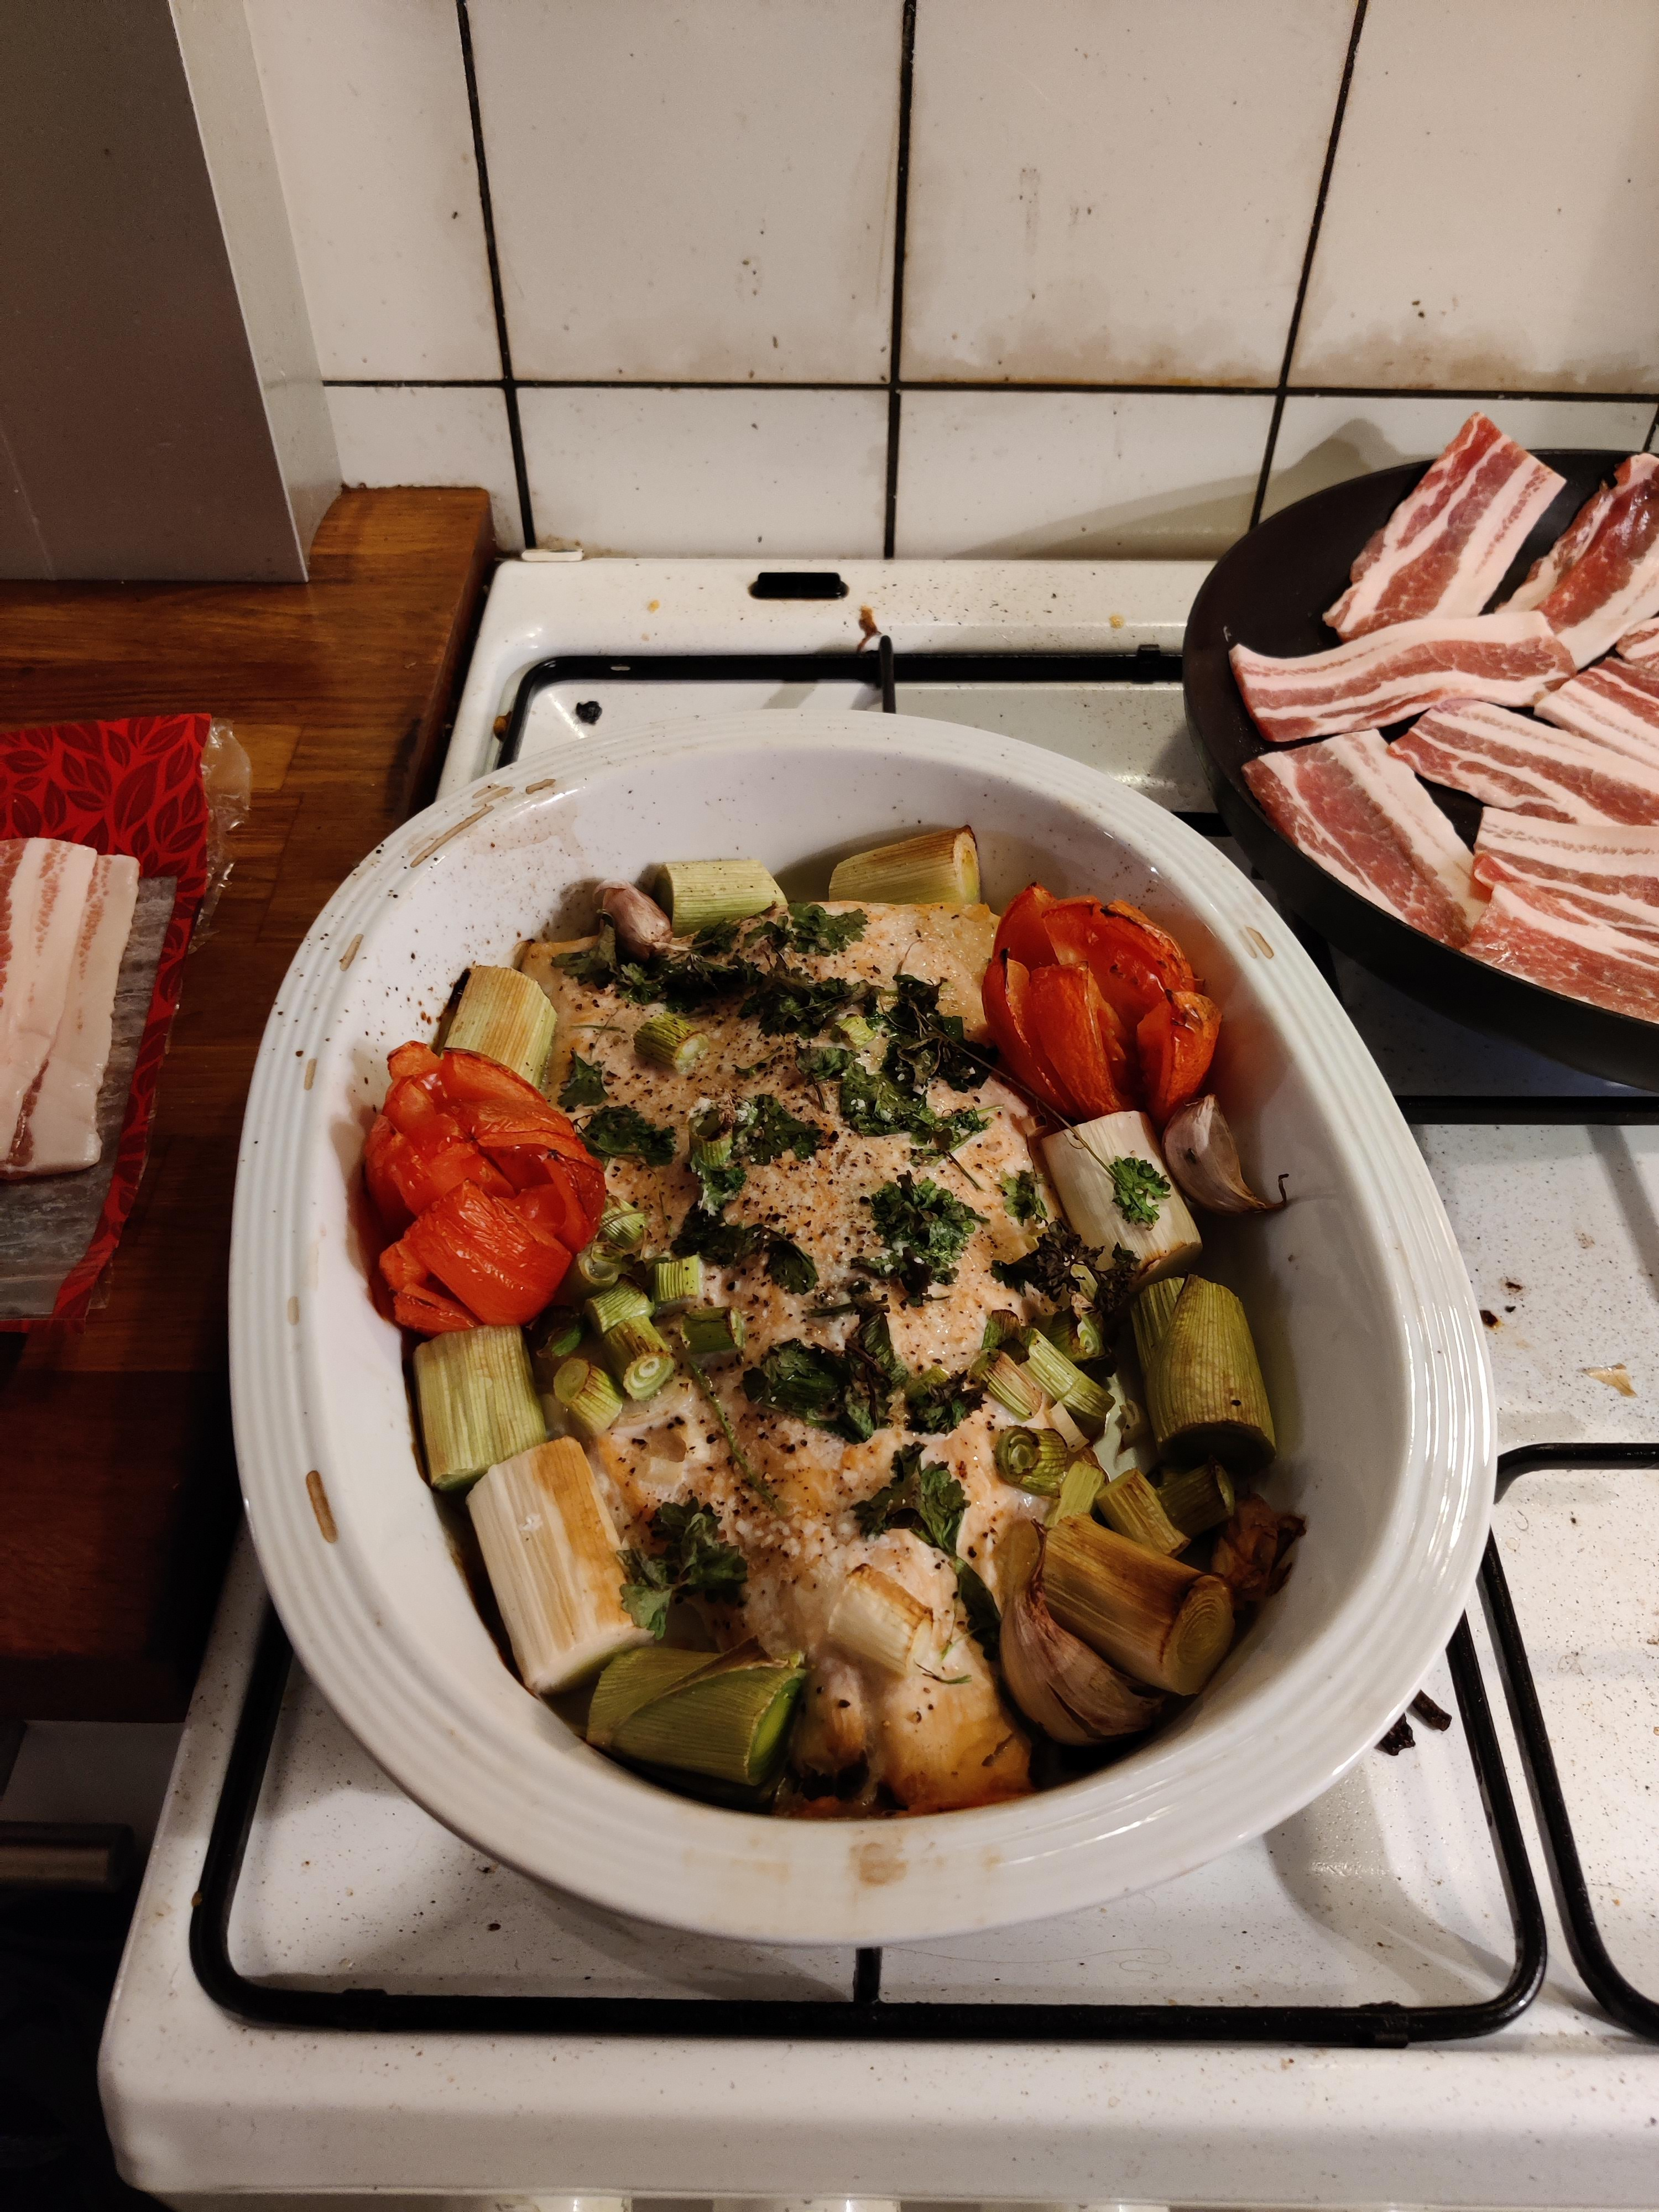
\includegraphics[width=\paperwidth,height=\paperheight]{Billeder/Aftensmad/Ovnbagt_laks.jpg}
    };
\end{tikzpicture}
\newpage \section{Moules Frittes}
\begin{minipage}[t]{0.5\textwidth}
\textbf{Ingredienser}
\begin{itemize}
    \item 500g blåmuslinger
    \item 2 tomatter
    \item 1 håndfuld korainder
    \item Pomfirtter
\end{itemize}
\end{minipage}
\begin{minipage}[t]{0.5\textwidth}
\textbf{Fremgangsmåde:}
\begin{enumerate}
    \item Hak tomatterne til tern.
    \item Skær koriander til små stykker.
    \item Skyld blåmuslingerne og sorter de dårlige blåmuslinger fra
    \item Kog blåmusinliger i en gryde med log, med tomatterne og korianderne.
    \item Sorter igen de dårlige blåmuslinger fra
\end{enumerate}
\end{minipage}
\\ \\ \\ 
Når blåmuslinger skal sorteres fra sker det i 2 faser, før de koges skal de skyldes, dem som ikke lukkes er allerede døde og skal frasorteres. Hvis der er synlige skader på blåmuslinger, såsom ødelagt skald ska disse også sortes fra. Efter de er kogte skal de blåmuslinger som ikke har åbnet sig også sorters fra.
\newpage
\begin{tikzpicture}[remember picture,overlay,inner sep=0pt,outer sep=0pt]
    \node[anchor=south east] at (current page.south east) {
        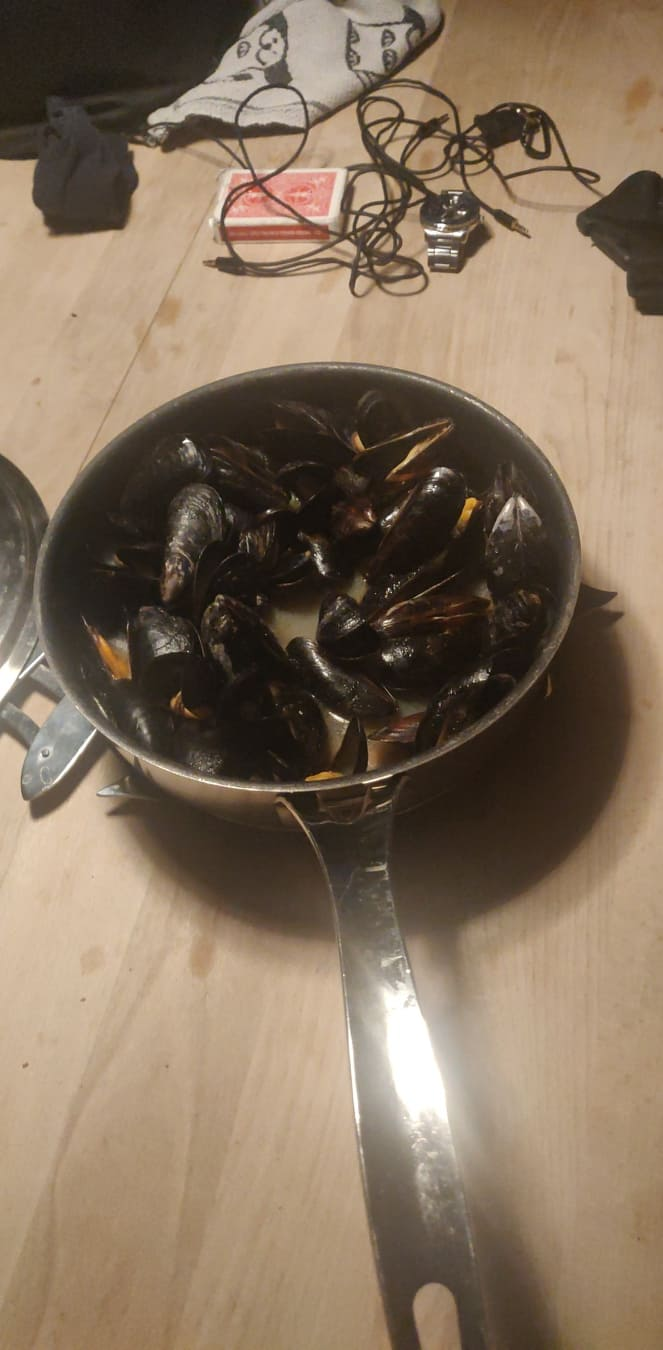
\includegraphics[width=\paperwidth,height=\paperheight]{Billeder/Aftensmad/Moulles_Frittes.jpeg}
    };
\end{tikzpicture}
\newpage \section{Stegt Flæsk med Persillesovs}
\begin{minipage}[t]{0.5\textwidth}
\textbf{Ingredienser:}
\begin{itemize}
    \item 700g flæsk i skiver
    \item 2 spsk hvedemel
    \item 5 dL mælk
    \item 1/2 citron, saft og skal herfra
    \item 2-3 håndfulde persille, finthakket
\end{itemize}
\end{minipage}
\begin{minipage}[t]{0.5\textwidth}
\textbf{Fremgangsmåde:}
\\Flæsken:
\begin{enumerate}
    \item Drys salt over flæsken, og lig på en rist
    \item Steg flæsken i oven ved 175 \degree C varmluft, og vend helst undervejs.
\end{enumerate}
Persillesovsen:
\begin{enumerate}
    \item Smelt smøren ved lav varme og pisk melen i, lidt efter lidt.
    \item Pisk mælken i ligeså.
    \item Kog saucen ved middel varme i cirka 5 minutter.
    \item Tilsæt det finthakket persille.
    \item Smag til med salt, pebber og citron.
\end{enumerate}
\end{minipage}
OBS. For at undgå et rod, andbefaler jeg at man beklæder en brædepande med bagepapir, som kan stå i bunden i ovnen.
\newpage 
\begin{tikzpicture}[remember picture,overlay,inner sep=0pt,outer sep=0pt]
    \node[anchor=south east] at (current page.south east) {
        \includegraphics[width=\paperwidth,height=\paperheight]{Billeder/Aftensmad/Stegt_Flæsk_Med_Persille_Sovs.jpeg}
    };
\end{tikzpicture}
\newpage \section{Stegte Ris}
\begin{minipage}[t]{0.5\textwidth}
\begin{itemize}
    \item 200g kogte ris
    \item 200g blandede grøntsager(vegtable mix eller wok mix fra netto)
    \item 100g mukimamme bønner
     \begin{enumerate}
        \item evt. Flere grøntsager hvis ønskede
        \item evt. Pandestegt spidskål (eventuelt stegt i goyang(koreansk chille pasta))
    \end{enumerate}
    \item 100g kylling
    \item Smør til stegning
    \item Soja til stegning
    \item 1 æg til stegning
\end{itemize}
\end{minipage}
\begin{minipage}[t]{0.5\textwidth}
\textbf{Fremgangsmåde:}
\begin{enumerate}
    \item Klargør grøntsagerne, tø grøntasger op, steg spidskållen osv, og steg kyllingen.
    \item Smør siden af en wok med smør, og put risene i ved høj varme.
    \item Tilsæt æg, til risene og rør grundigt rundt, det vigtigt at ægenne ikke blvier spejlet
    \item tilsæt grøntsagerne, kyllingen og soja saucen og steg under omrøring.
    \item Når risene har fået en brun farve, og ikke er klistret er de good to go
\end{enumerate}
\end{minipage}
\newpage   Heg har jeg igen glemt at tage et billede, så i mellemtiden er der et billede af mig på en sushi resturent \begin{figure}
    \centering
    
\includegraphics[width=0.5\linewidth]{Sushi_spisning.jpg}
    \caption{Et billede af mig på CC sushi resturent på Åboulevarden}
\end{figure}
\newpage \section{T'uhu}
Sumerisk lam og rødbede gryderet, som er den ældste kendte opskrift, estimeret at være flere tusind år gammel.

\begin{minipage}[t]{0.5\textwidth}
\textbf{Ingredienser:}
\begin{itemize}
    \item 500g Fedtrigt lam i tern (Egentlig fårkød men det pænt svært at få)
    \item 100 mL Fårfedt (eller kokosolie)
    \item 1 løg
    \item 1 tsk salt
    \item 500g Rødbedder i tern
    \item 100g hakket rucola
    \item Frisk koriander
    \item 125g hakket skalotteløg
    \item 1 tsk spidskommen frø
    \item 100mL Weissbier
    \item 50 mL vand
    \item 75g hakket porrer
    \item 3 fed hvidløg
\end{itemize}
\underline{Tilbehør:}
\begin{itemize}
    \item 75g friske hakkede koriander
    \item 75g forårsløg
    \item 2 tsk spidskommen frø
\end{itemize}
\end{minipage}%
\begin{minipage}[t]{0.5\textwidth}
\textbf{Fremgangsmåde:}
\begin{enumerate}
    \item Varm kokosolie (eller andet fedt) i en gryde bred nok til det hakkede lam, i et lag.
    \item Svitser lammet indtil al væsken er væk.
    \item Tilsæt løgene og steg indtil de er gennemsigtige.
    \item Tilsæt derefter salt, rødbeder, rucola, koriander, skalotteløg og spidskommenfrø, og steg indtil væsken er væk.
    \item Tilsæt ølen, vandet og bring det i kog.
    \item Tilføj løg og porrer og lad det simre i en times tid.
\end{enumerate}
\underline{Tilbehør:}
\begin{enumerate}
    \item Knus foråsløgene og korianderne i en morter eller lignende og drys spidskommenfrøene på.
\end{enumerate}
\end{minipage}
\footnote{Kilde: \href{https://www.bbc.com/travel/article/20191103-the-worlds-oldest-known-recipes-decoded}{BBC travel}}
\newpage
\begin{tikzpicture}[remember picture,overlay,inner sep=0pt,outer sep=0pt]
    \node[anchor=south east] at (current page.south east) {
        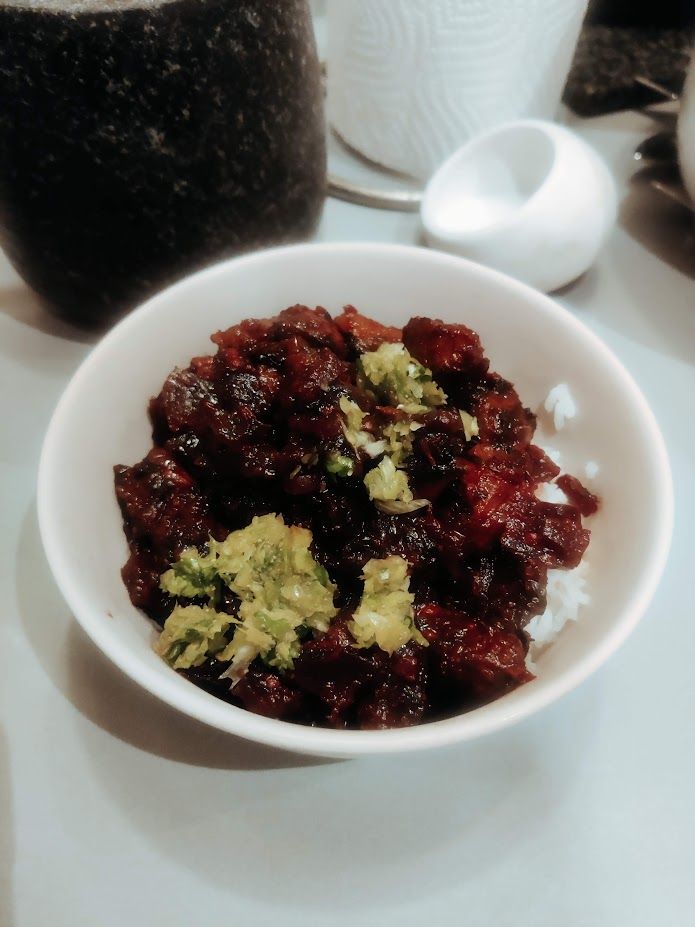
\includegraphics[width=\paperwidth,height=\paperheight]{Billeder/Aftensmad/Tuhu.jpg}
    };
\end{tikzpicture}
\chapter{Vegetarisk Aftensmad}
\minitoc 
\newpage \section{Arabiatta}
\begin{minipage}[t]{0.5\textwidth}
\textbf{Ingredienser:}
\begin{itemize}
    \item 1 dåse flåede tomatter
    \item 3 spsk olivenolie
    \item 1 tsk balsamico
    \item 1 tsk sukker
    \item Citronsaft
    \item 1-2 håndfuld basilikum
    \item 1/2 tsk chiliflager 
    \item 2-3 presset fed hvidløg
    \item 1 finthakket løg
\end{itemize}
\end{minipage}
\begin{minipage}[t]{0.5\textwidth}
\textbf{Fremgangsmåde:}
\begin{enumerate}
    \item Svits løgnene i olien.
    \item Tilsæt hvidløg, tomatter, sukker og basilikum.
    \item Smag til med balsamico, salt og peber
\end{enumerate}
\end{minipage}
\newpage Her mangler der så også et billede desværre, så her er endnu et billede fra Sverige turen.
\begin{figure}
    \centering
    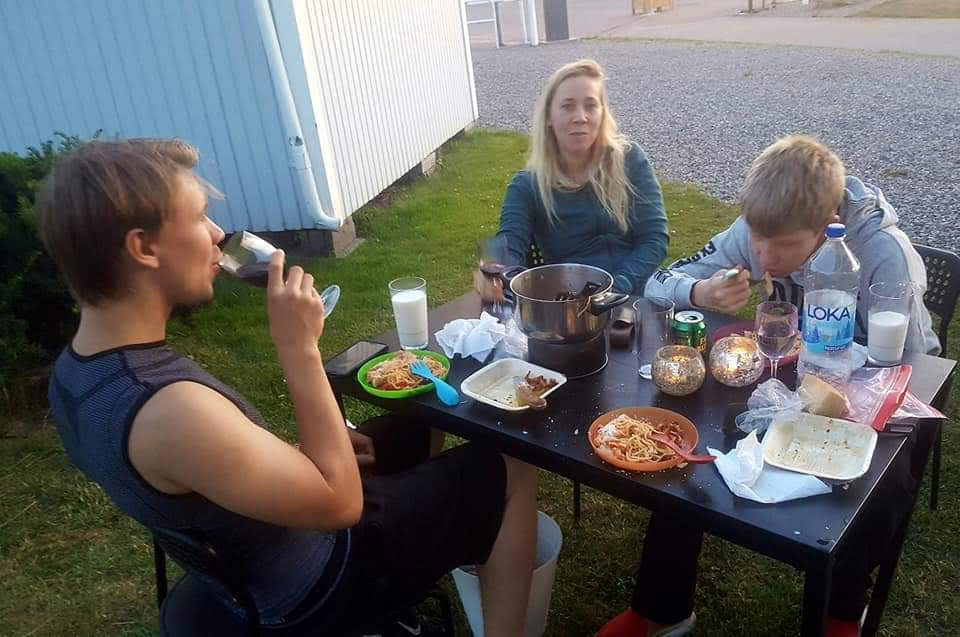
\includegraphics[width=0.5\linewidth]{Sverigept1.jpg}
    \caption{Sverige pt 1}
    
\end{figure}
\newpage \section{Dhal}
\begin{minipage}[t]{0.5\textwidth}
\textbf{Ingredienser} \\
\underline{Dhal}
\begin{itemize}
    \item 4 fed hvidløg
    \item 2 løg
    \item 2 spsk frisk revet ingefær, eller 2 tsk tørret
    \item 2 spsk olivenolie
    \item 200 gram tørre røde linser
    \item 2 dåser hakkede tomatter
    \item Kryderier
    \begin{enumerate}
        \item 6 dL grøntsagsbouillon
        \item 0.5 tsk chiliflager
        \item 0.5 tsk stødt kardemonne
        \item 0.5 spsk stødt koriander
        \item 1 spsk stødt spidskommen
        \item 0.5 tsk garam masala
        \item 0.5 tsk paprika
    \end{enumerate}
    \end{itemize} 
\underline{Raita:}
\begin{itemize} 
    \item 1 håndfuld mynte
    \item 2 dL græsk yoghurt
    \item 0.5 agurk, mandolin revet
    \item 2 fed hvidløg
    \item spidskommen
    \item salt og peber
    \item Eventuelt
    \begin{itemize}
        \item Citronsaft eller limesaft
    \end{itemize}
\end{itemize}
\end{minipage}
\begin{minipage}[t]{0.5\textwidth}
\textbf{Fremgangsmåde} \\
\underline{Dhal} 
\begin{enumerate}
    \item Svits løg, hvidløg og krydderier i olien
    \item Tilsæt, grøntsagsbouillon, vaskede linser og de hakkede tomatter
    \item Bring op og koge, og lad simre i mindst 30 minutter, konsistensen kan reddes med eventuel flere linser (hvis den er for flydende) eller mere vand (hvis den er for fast). Smag til med salt og pebber
\end{enumerate}
\underline{Raita:}
\begin{enumerate}
    \item Riv agurken i tykke skive og dræn vandet derfra
    \item skær mynten ude i små stykker
    \item Mix ingredienserne sammen og samg til med salt og peber
\end{enumerate}
\end{minipage}
\\ \\ \\ \underline{Noter:}
Der kan sagtens bruges våde linser (fra en dåse), men så skal der bruges markant mindre væske. \\ Til servevingen kan den pyntes med friske koriander, eller eventuelt ristede græskarkerner.  \\ Dhal kan sagtens spises for sig selv, men kan også nydes med enten naan brød, eller ris.


\newpage
\begin{tikzpicture}[remember picture,overlay,inner sep=0pt,outer sep=0pt]
    \node[anchor=south east] at (current page.south east) {
        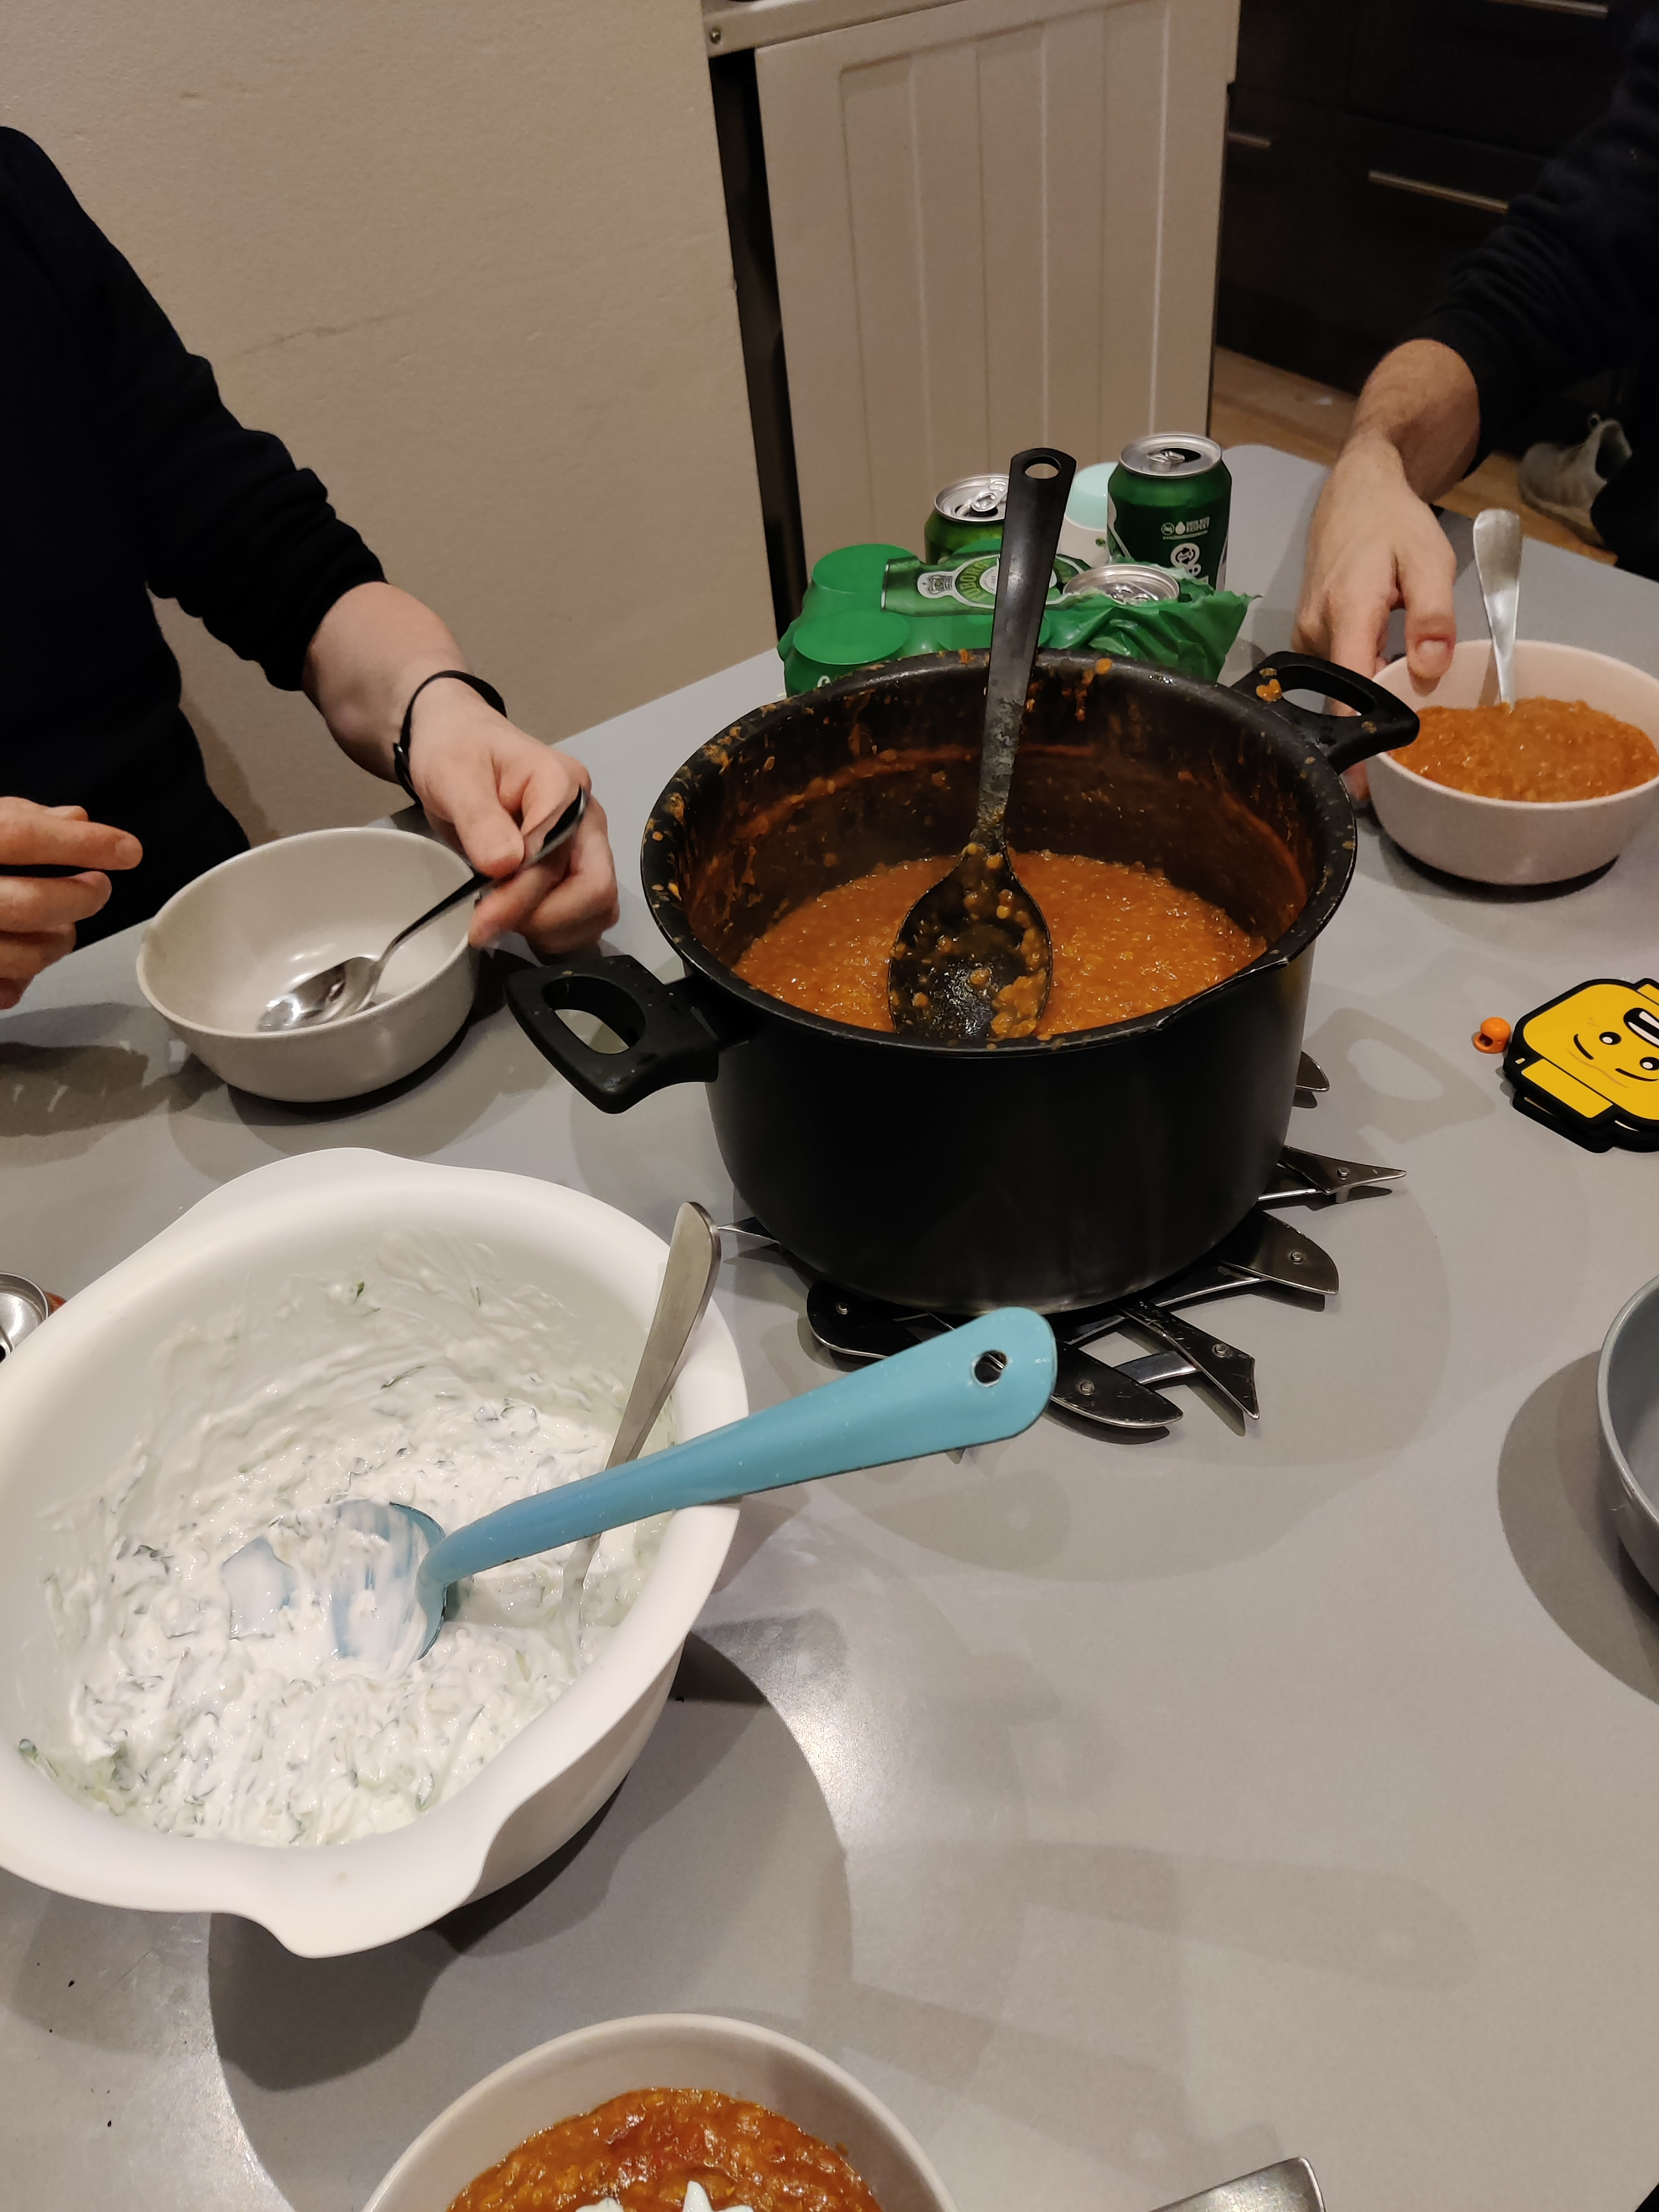
\includegraphics[width=\paperwidth,height=\paperheight]{Billeder/Aftensmad/Dahl.jpg}
    };
\end{tikzpicture}
\newpage \section{Kartoffel porre suppe}
\begin{minipage}[t]{0.5\textwidth}
\textbf{Ingredienser:}
\begin{itemize}
    \item 500g kartofler
    \item 3 porrer, skårret i ringe
    \item 1 løg, finthakket
    \item 20 g smør
    \item 3/4 L grøntsagsbouillon
    \item 1 dL piskefløde
    \item salt og peber
\end{itemize}
\textbf{Tilbehør og topping}
\begin{itemize}
    \item 150g bacon i tern
    \item Frisk timian
    \item Brød
\end{itemize}
\end{minipage}
\begin{minipage}[t]{0.5\textwidth}
\textbf{Fremgangsmåde:}
\begin{enumerate}
    \item Smelt smørret og svits kartofler, løg og porrer i 2-3 minutter
    \item Tilsæt grøntsagsbouillon, og lad koge i omtrent 15 minutter, til kartoflerne er møre.
    \item Blend kartoflerne i stykker med stavblender
    \item Tilsæt piskefløde og kog op, samg til med salt og pebber
\end{enumerate}
\end{minipage}
\newpage Her mangler jeg sku igen et billede, så her er et billede af mig i en kenguru 
\begin{figure}
    \centering
    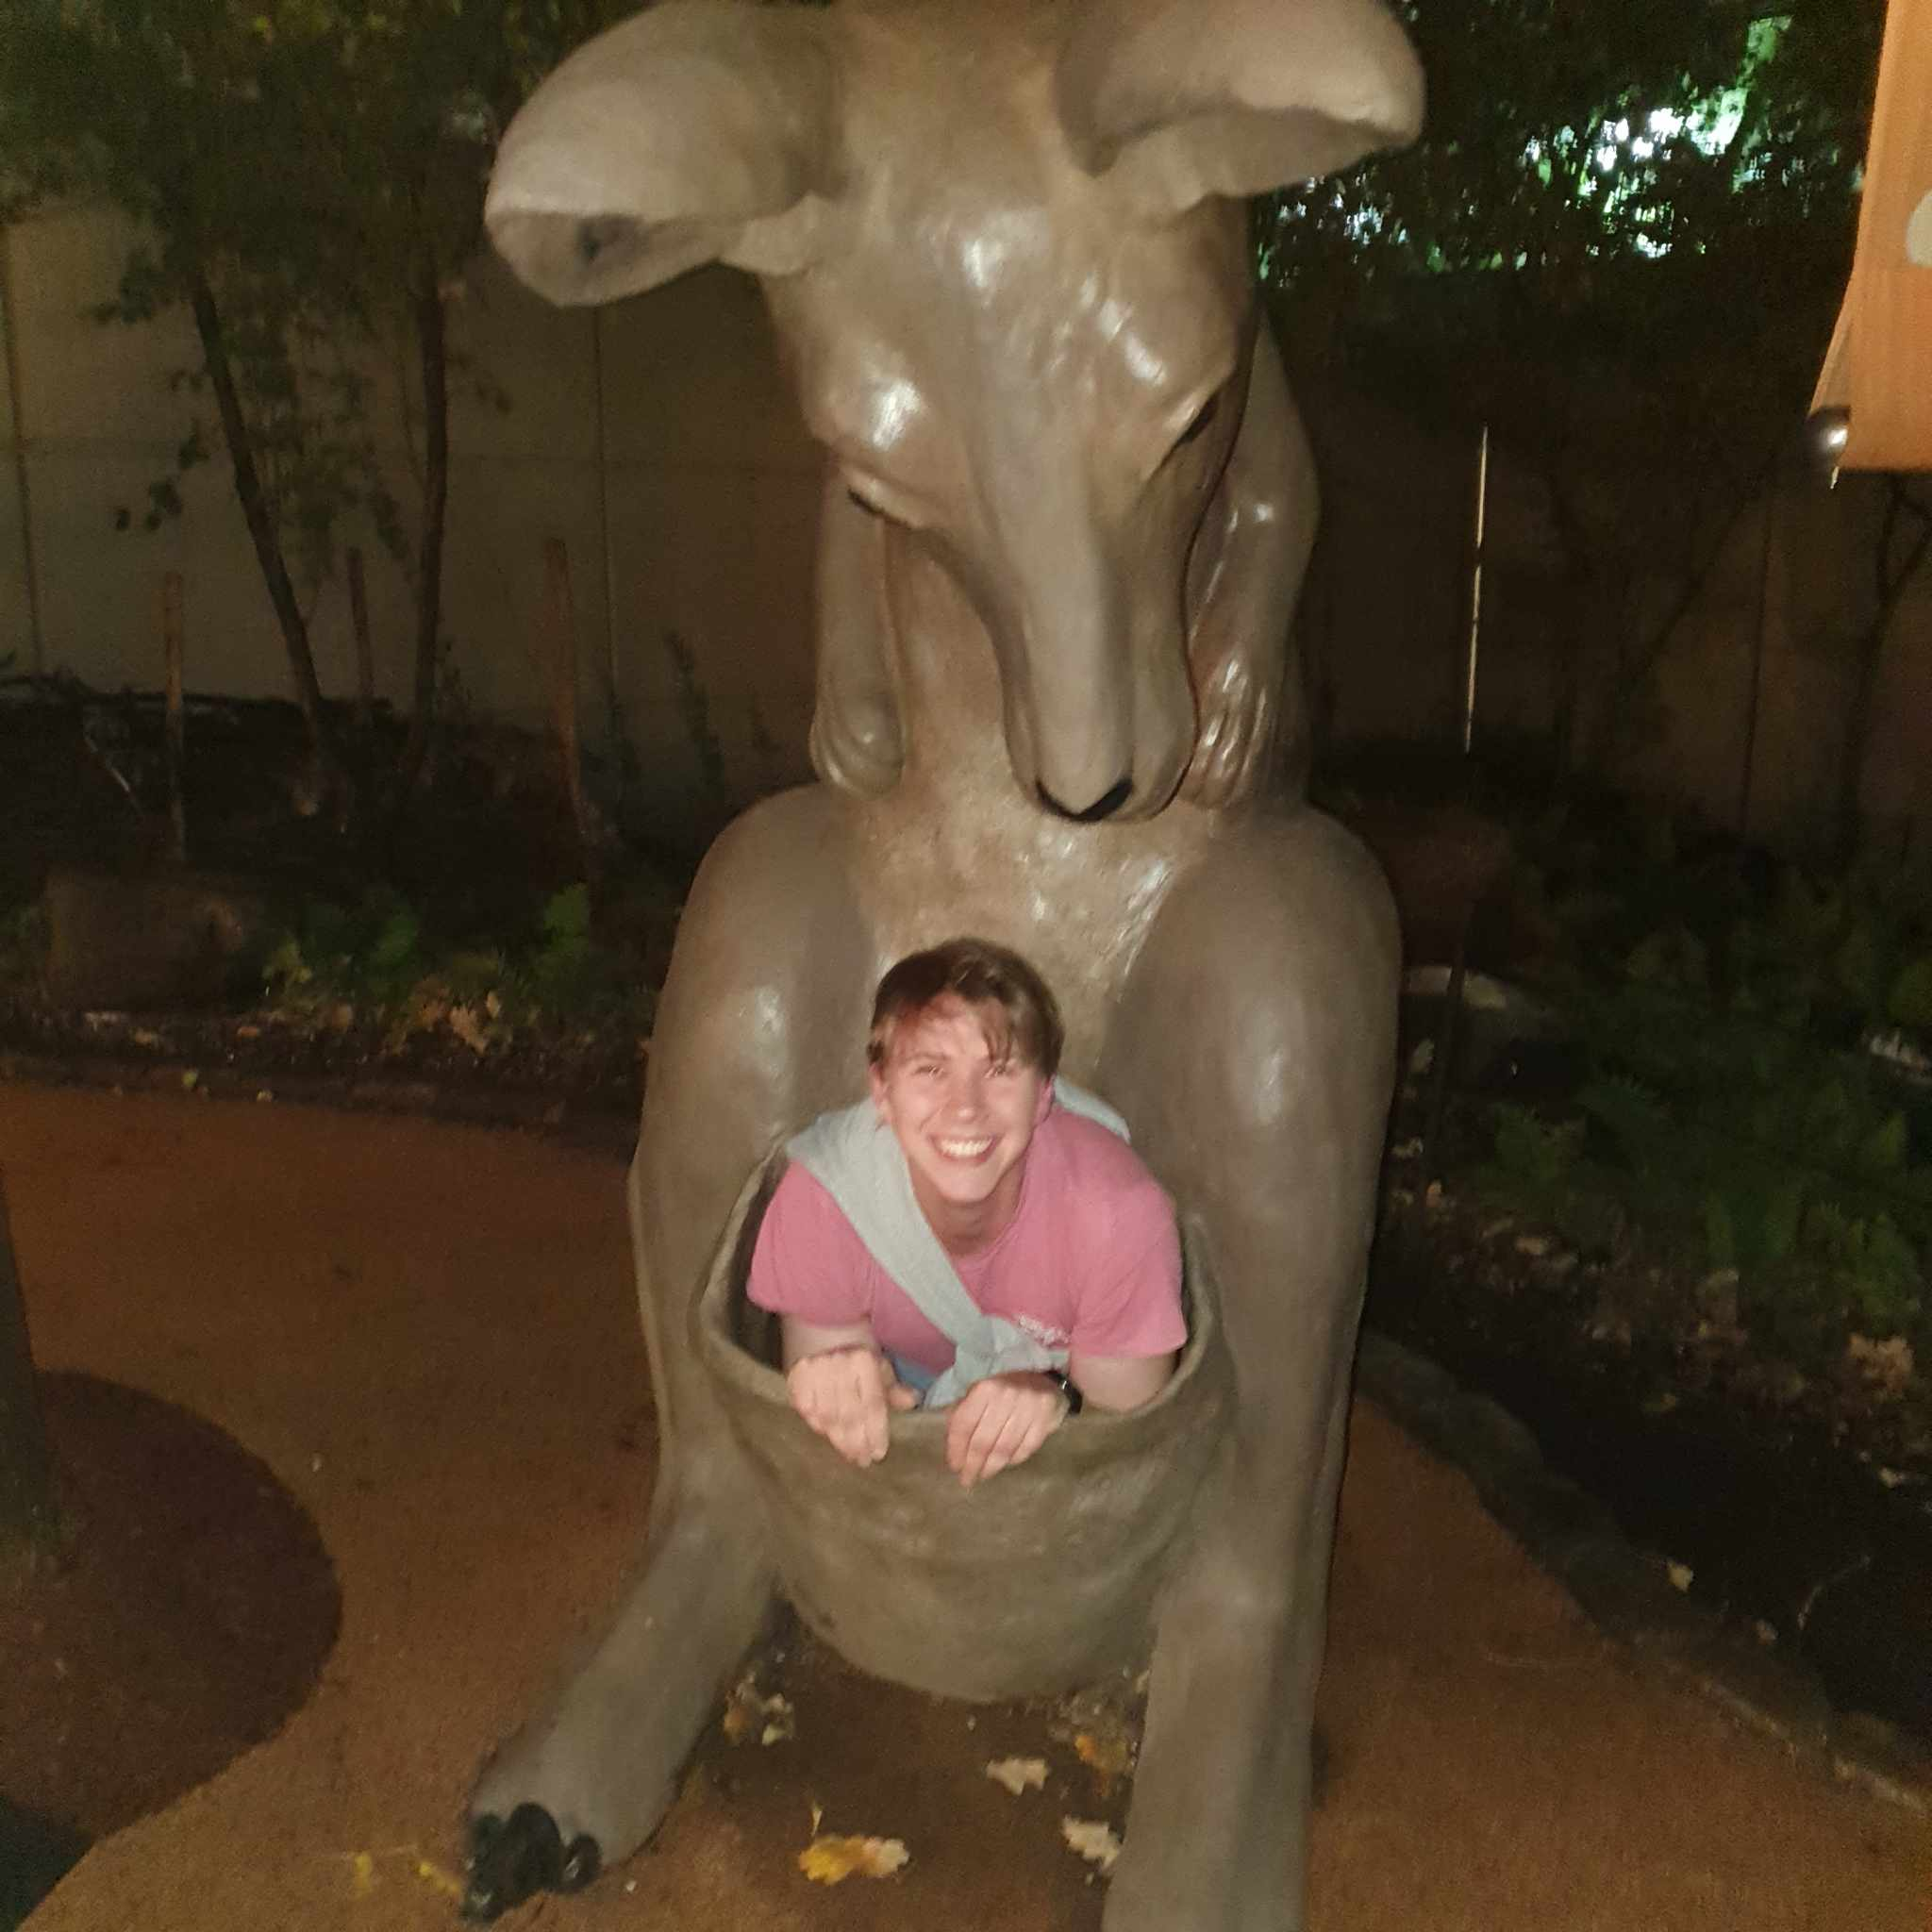
\includegraphics[width=0.5\linewidth]{Kenguru.jpeg}
    \caption{Kulturnat i 2023}
    
\end{figure}
\newpage \section{Løgsuppe}
\begin{minipage}[t]{0.5\textwidth}
\textbf{Ingredienser}
\begin{itemize}
    \item 500 g løg 
    \item 4-6 fed hvidløg
    \item timian
    \item salt og peber
    \item 1 L grøntsagsbulijon 
    \item Eventuelt krydderi
    \begin{enumerate}
        \item Chiliflager
        \item Cayennepeber
        \item Rosmarin
    \end{enumerate}
\end{itemize}
\end{minipage}
\begin{minipage}[t]{0.5\textwidth}
\textbf{Fremgangsmåde:}
\begin{enumerate}
    \item Svits løgne til gyldne og tilsæt krydderier
    \item Tilsæt dernæst grøntsagsbuljion og kog op
    \item Lad simre i mindst 20 minutter
\end{enumerate}
\end{minipage}
Hvis man smider løgne i en food proccessor, bliver suppen en anelese flydende, men smagen er der stadigvæk.
\newpage 
Her har jeg så igen glemt at tage et billede, så istedet for mig der spiser løgsuppe, er der mig som drikker mad på fad i mBAR.
\begin{figure}
    \centering
    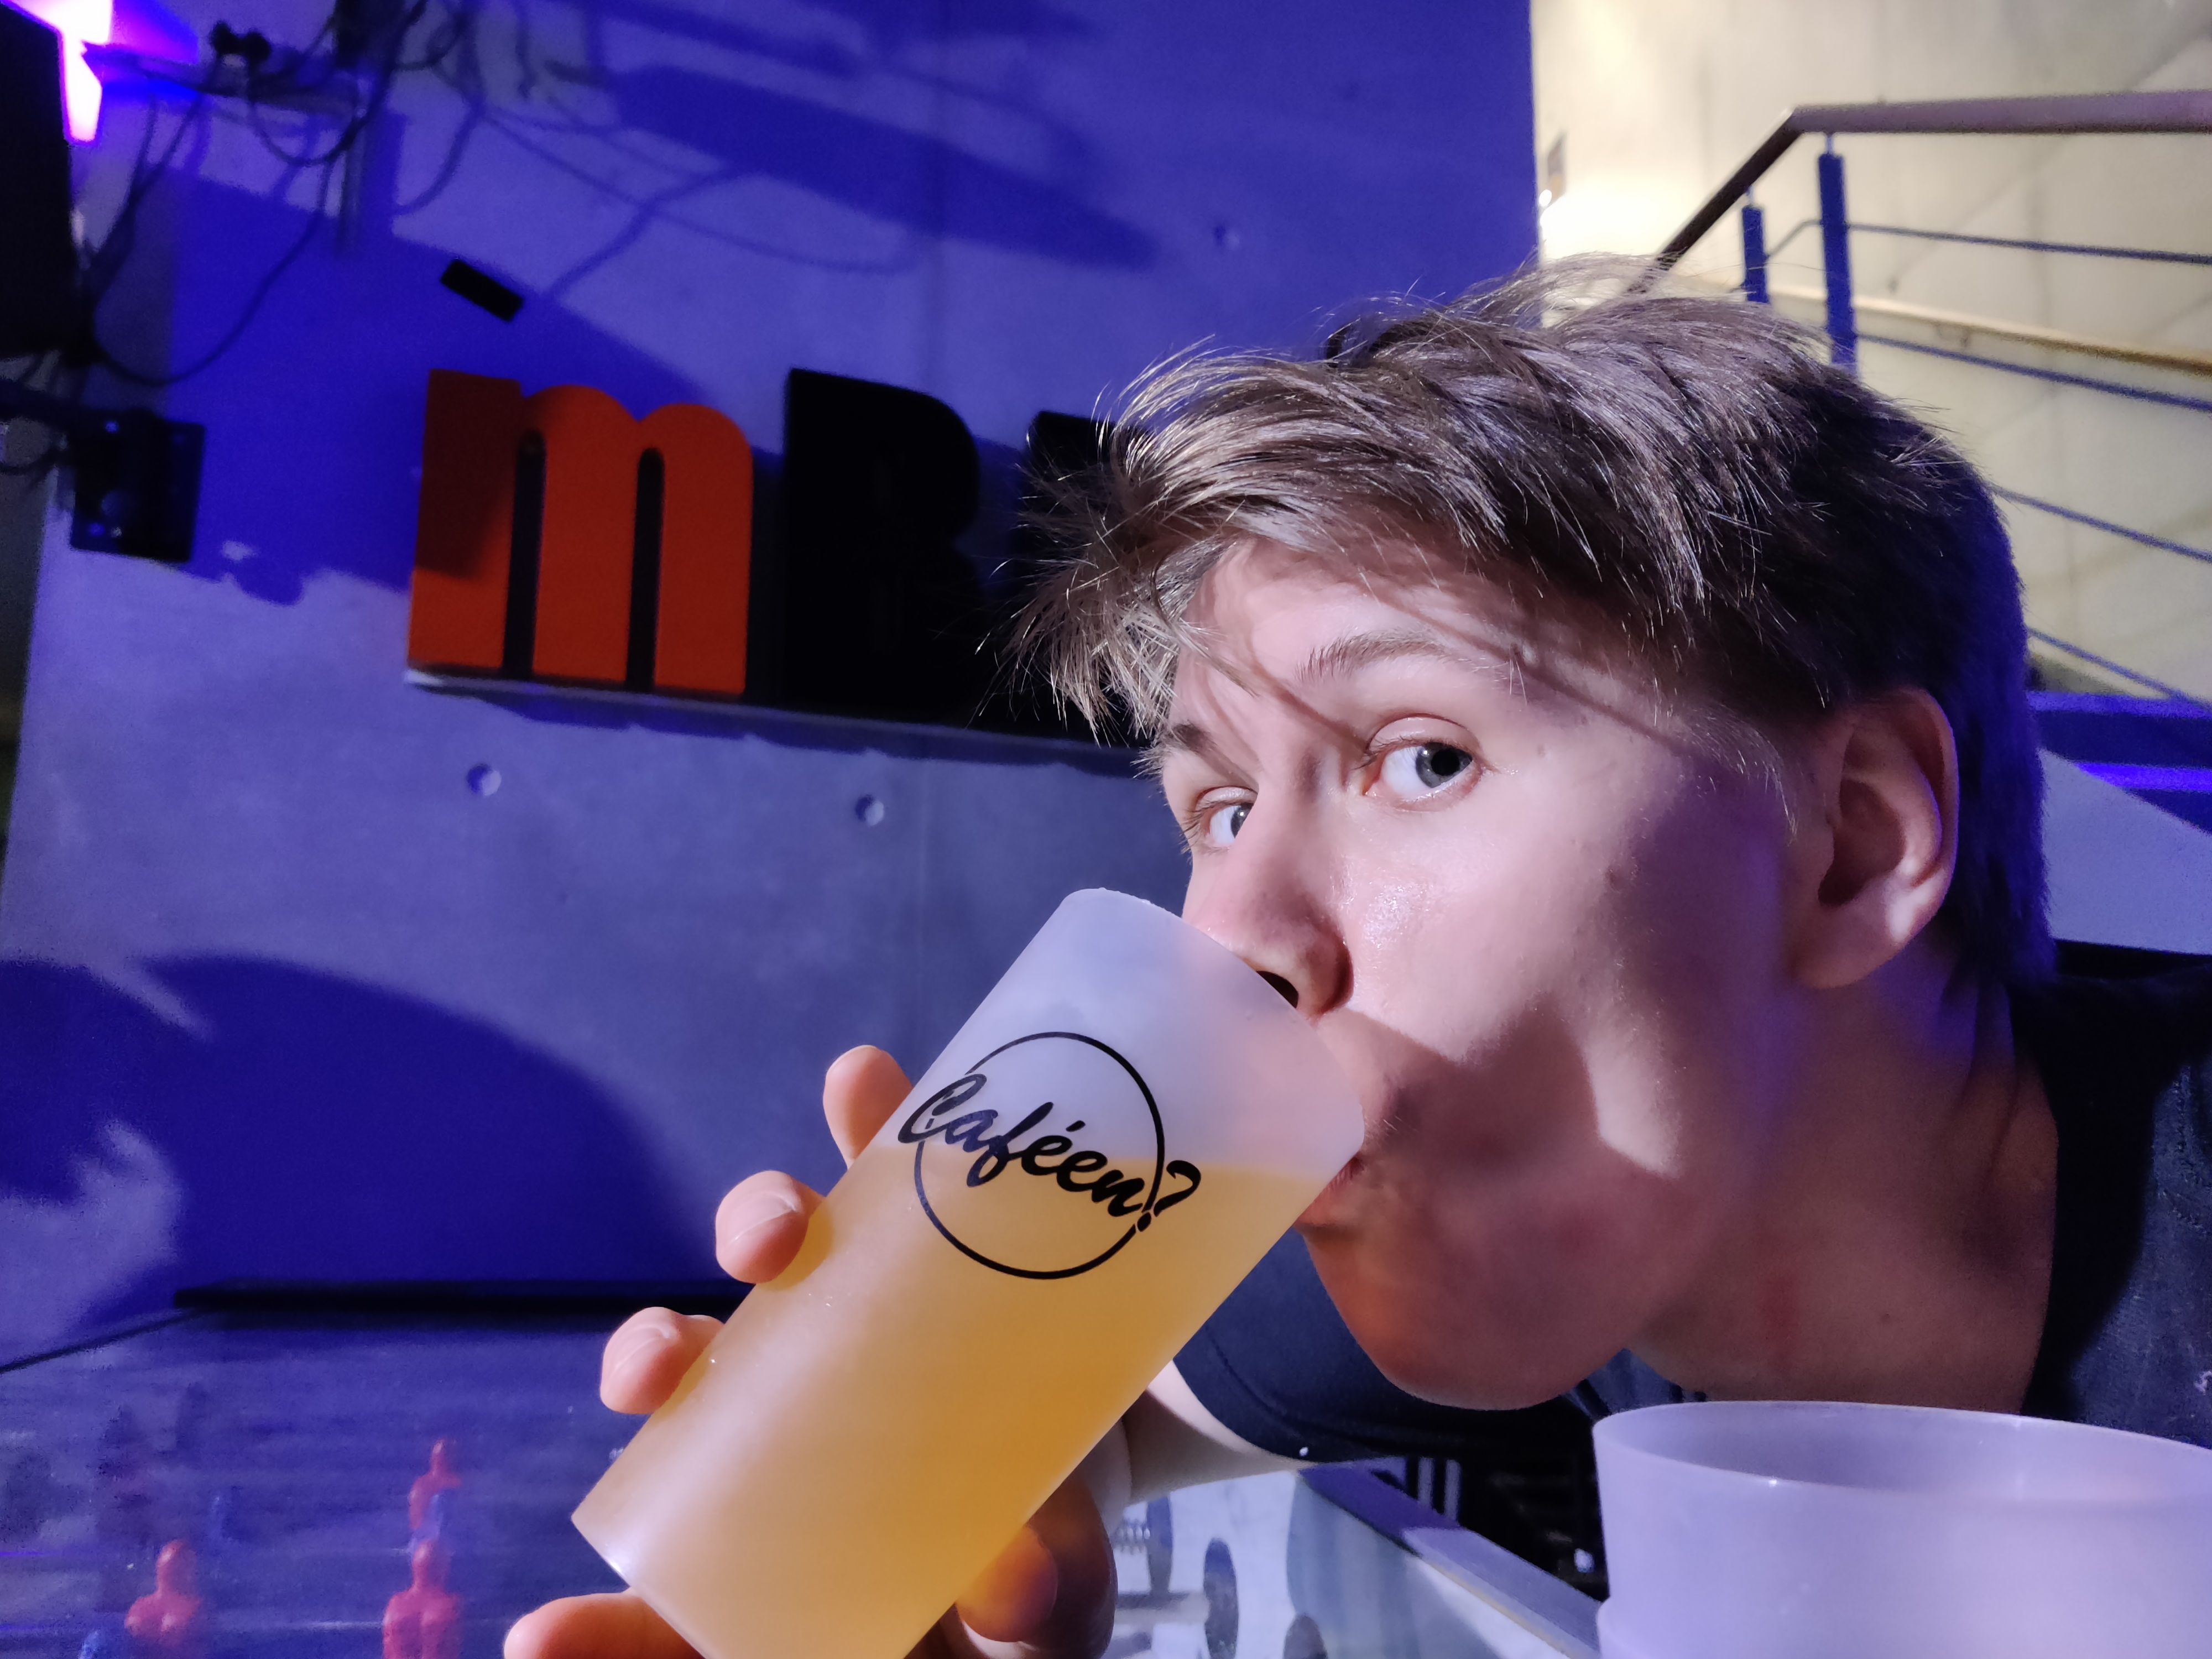
\includegraphics[width=0.5\linewidth]{mBAR.jpg}
    \caption{Mig i mBAR}
    
\end{figure}
\newpage 
\section{Ovnbagt aubergine}
\begin{minipage}[t]{0.5\textwidth}
\begin{itemize}
    \item 1 aubergine
    \item 10 g smør
    \item 1 fed hvidløg
    \item frisk timian
    \item salt og pebber
\end{itemize}
\end{minipage}
\begin{minipage}[t]{0.5\textwidth}
\textbf{Fremgangsmåde:}
\begin{enumerate}
    \item Skær auberginen over på midten (oppe fra ned), og scoop \~ 1 skefuld aubergine kød ud.
    \item Rids fordybningen minimalt så smagen kan synke ind.
    \item Pak dem ind i sølvpapir i smid i ovnen på 200 \degree C varmluft i 15 minutter
    \item Når auberginerne er færdig skal de gerne være let brundet, og halvsprøde i overfladen.
\end{enumerate}
\end{minipage}
Det er let at opskallere opskrift til flere aubergine, det vigtigste er at auberginerne er af nogenlunde størrelse. Hvidløget kan enten presses og dermed blive i, eller masses til større stykker så saften blandetsig med smøren.
\newpage 
Fremfor et billede af en lækker aubergine, kommer der istedet for et billede fra Biokemi galla 2023
\begin{figure}
    \centering
    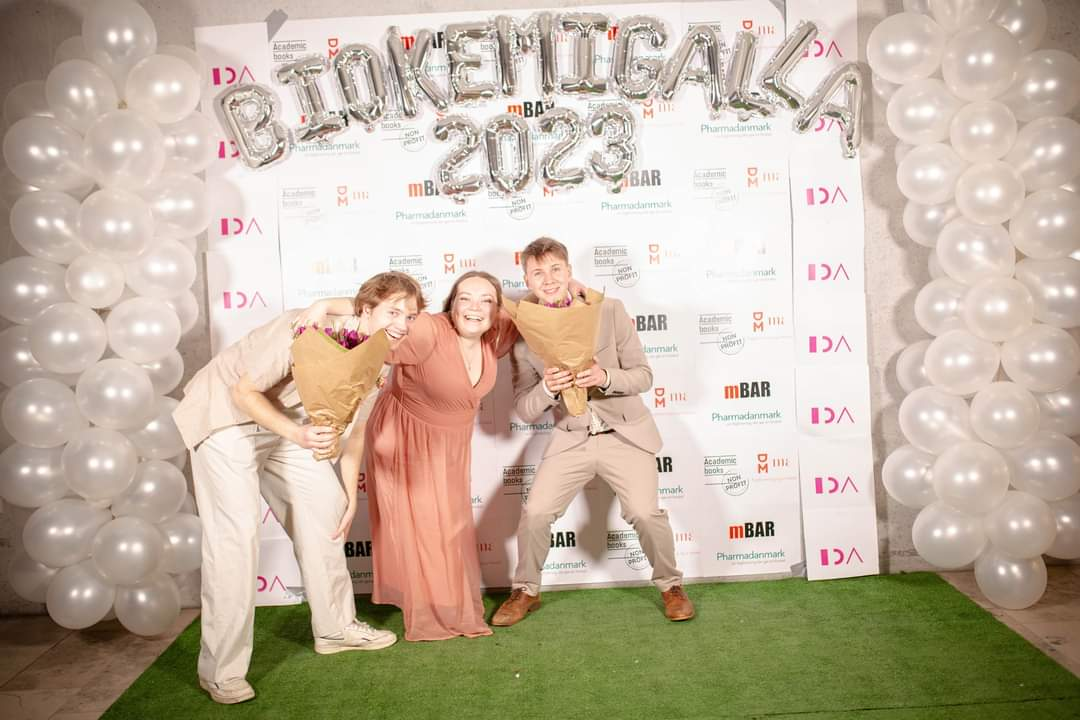
\includegraphics[width=0.5\linewidth]{Galla.jpg}
    \caption{Billedet fra biokemigalla 2023}
\end{figure}
\newpage \section{Ovnbagte søde kartofler}
Til retten anbefaler jeg søde kartofler cirka på størrelse med bagekartofler, da dette giver en bedre mulighed for at fylde den ud. Rettens skal lidt ses som en sødekartoffelmos, som der stadig er i dens skrald. Man kan med fordel tilfje flere grøntsager som fylld, men dette er min umiddelbare anbefaling\\
\begin{minipage}[t]{0.5\textwidth}
\textbf{Ingredienser:}
\begin{itemize}
    \item 2-3 Søde kartolfer
    \item Smeltet smør
    \item Hvidløg
\end{itemize}
\underline{Fyldet:}
\begin{itemize}
    \item Avokado 
    \item Pico de Gallo
    \item Bønnepasta
    \item Græsk yoghurt dressing 
\end{itemize}
\end{minipage}
\begin{minipage}[t]{0.5\textwidth}
\begin{enumerate}
    \item Skær ridser i de søde kartofler og såleddes at smøren og hvidløgen kan sive ned i.
    \item Bag i ovnen i omtrent 1 time ved ved 180 C°, til blød i midten.
    \item Mos kartofflen delvis og bland fyldet ned i kartoflen, jeg bleger at genopfylde løbende.  
\end{enumerate}
\end{minipage}
\newpage
\begin{tikzpicture}[remember picture,overlay,inner sep=0pt,outer sep=0pt]
    \node[anchor=south east] at (current page.south east) {
        \includegraphics[width=\paperwidth,height=\paperheight]{Billeder/Aftensmad/Ovnbagt_sødkartoffel.jpg}
    };
\end{tikzpicture}
\newpage \section{Ratatoulie}
\begin{minipage}[t]{0.5\textwidth}
\textbf{Ingredienser:}
\\ Til Sovsen:
\\ Til sovsen kan man passende bruge min opskrift på arabiatta (det plejer jeg hvertfald)
\begin{itemize}
    \item 1 dåse flåede tomatter
    \item 3 spsk olivenolie
    \item 1 tsk balsamico
    \item 1 tsk sukker
    \item Citronsaft
    \item 1-2 håndfuld basilikum
    \item 1/2 tsk chiliflager 
    \item 2-3 presset fed hvidløg
    \item 1 finthakket løg
\end{itemize}
Til Toppen:
\begin{itemize}
    \item Tomatter
    \item Aubergine
    \item Squash 
\end{itemize}
Dressing:
\begin{itemize}
    \item Olivenolie
    \item Frisk Timian
\end{itemize}
\end{minipage}
\begin{minipage}[t]{0.5\textwidth}
\textbf{Fremgangsmåde}
    \begin{enumerate}
        \item Hæld tomatsovsen i et fad (omtrent 3-4 centimeter)
        \item Skær grøntsagerne ud i skiver, ikke for tynde.
        \item Aranger skiverne i mønster oven på tomatsovsen i fadet.
        \item Drys olivenoie dressingen oven på
   \end{enumerate}

\end{minipage}
Til ratatoullien er det vigtigt at vælge gode grøntsager til toppen, jeg er personlig fan af de 3 overstående men man kan sagtens vælge andet, jeg vil dog fraråde at bruge, butternut squash og andre former for græskar da de ikke får den ønskede konsistens. Jeg har endnu ikke fået det til at ligne ratatouille som set i dokumentar filmen Ratatouille 
\newpage
\begin{tikzpicture}[remember picture,overlay,inner sep=0pt,outer sep=0pt]
    \node[anchor=south east] at (current page.south east) {
        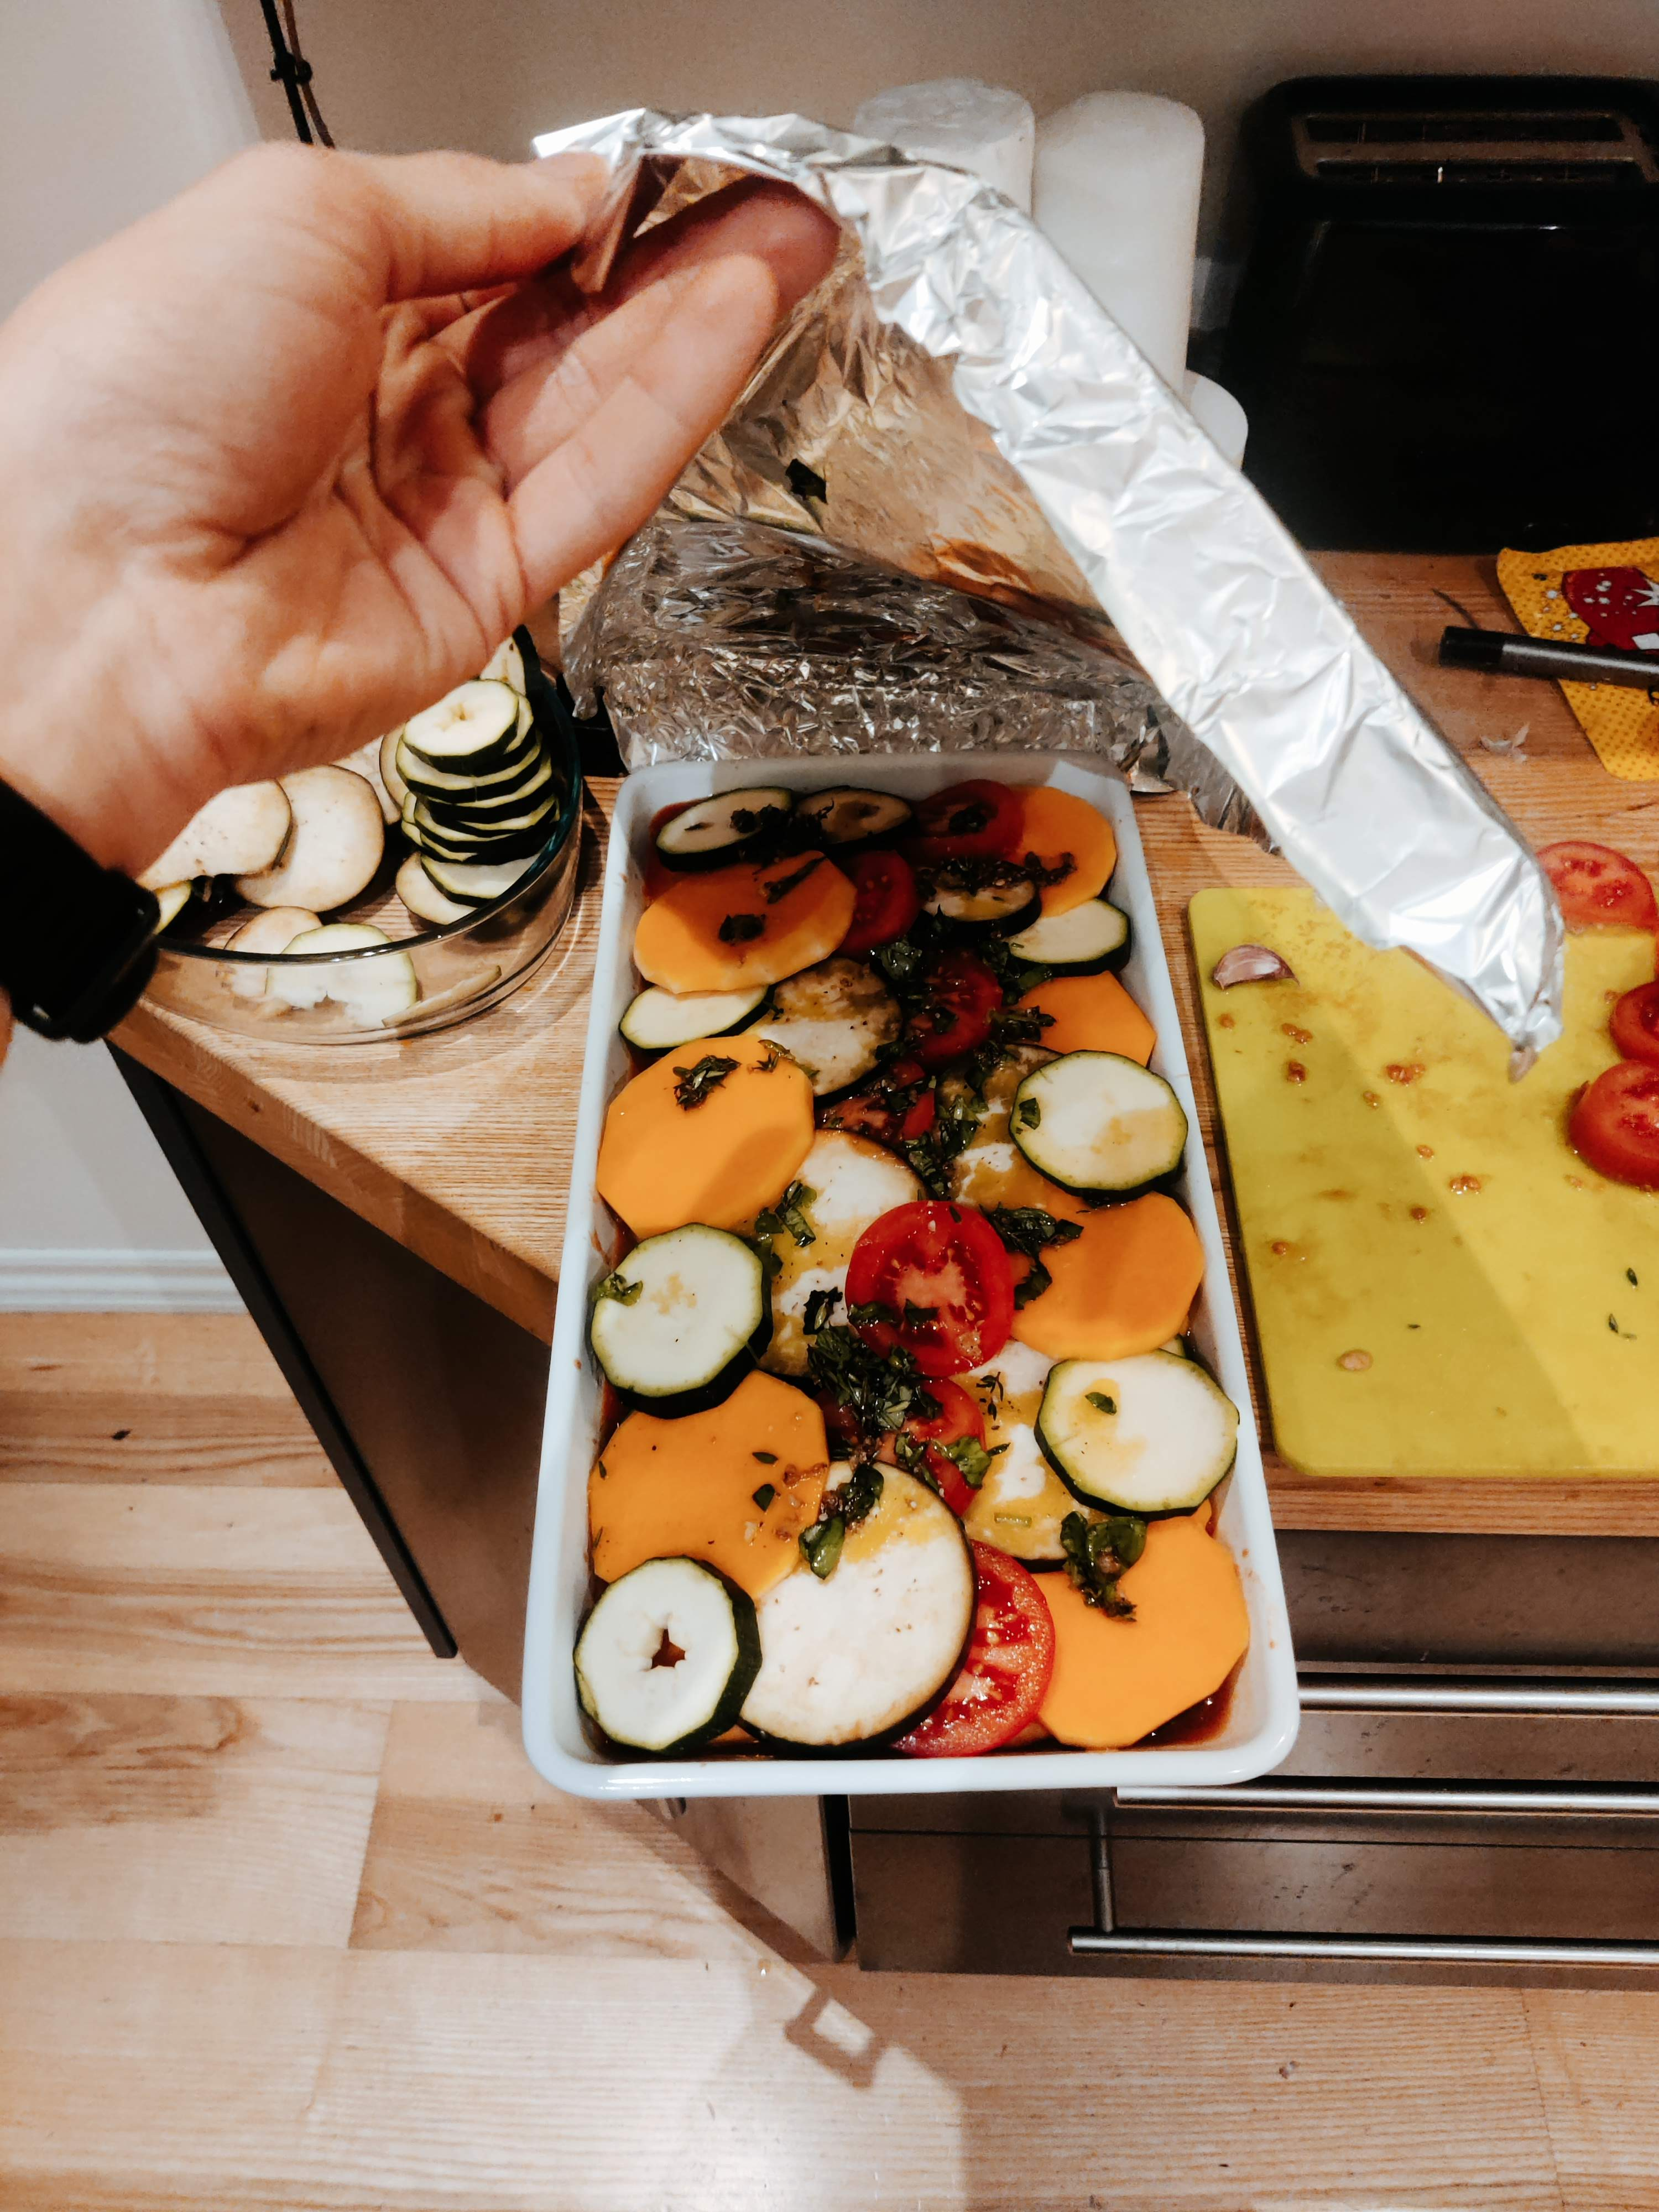
\includegraphics[width=\paperwidth,height=\paperheight]{Billeder/Aftensmad/Ratatoulie.jpg}
    };
\end{tikzpicture}
\newpage 
\section{Risotto Svampe}
\begin{minipage}[t]{0.5\textwidth}
\textbf{Ingredienser:}
\begin{itemize}
    \item 1 løg, finthakket
    \item 1 fed hvidløg, finthakket
    \item 400 g risotto ris
    \item 300 g champignon
    \item 1 L grøntsagsbouillon
    \item 50 g parmesan, friskrevet
    \item 1 dL piskefløde
    \item 20 g smør
\end{itemize}
\end{minipage}
\begin{minipage}[t]{0.5\textwidth}
\textbf{Fremgangsmåde:}
\begin{enumerate}
    \item Svits løgne og hvidløgne til gyldne.
    \item Tilsæt rissotorisen, vin og 300 mL grøntsagsbouillon.
    \item Tilsæt resten af grøntsagsbuilloinen lidt efter lidt, til rissene er møre (ca 20 minutter).
    \item Vend osten og fløden i, og lad osten smelte under konstant omrøring.
\end{enumerate}
\end{minipage}
\newpage  \newpage \begin{tikzpicture}[remember picture,overlay,inner sep=0pt,outer sep=0pt]
    \node[anchor=south east] at (current page.south east) {
        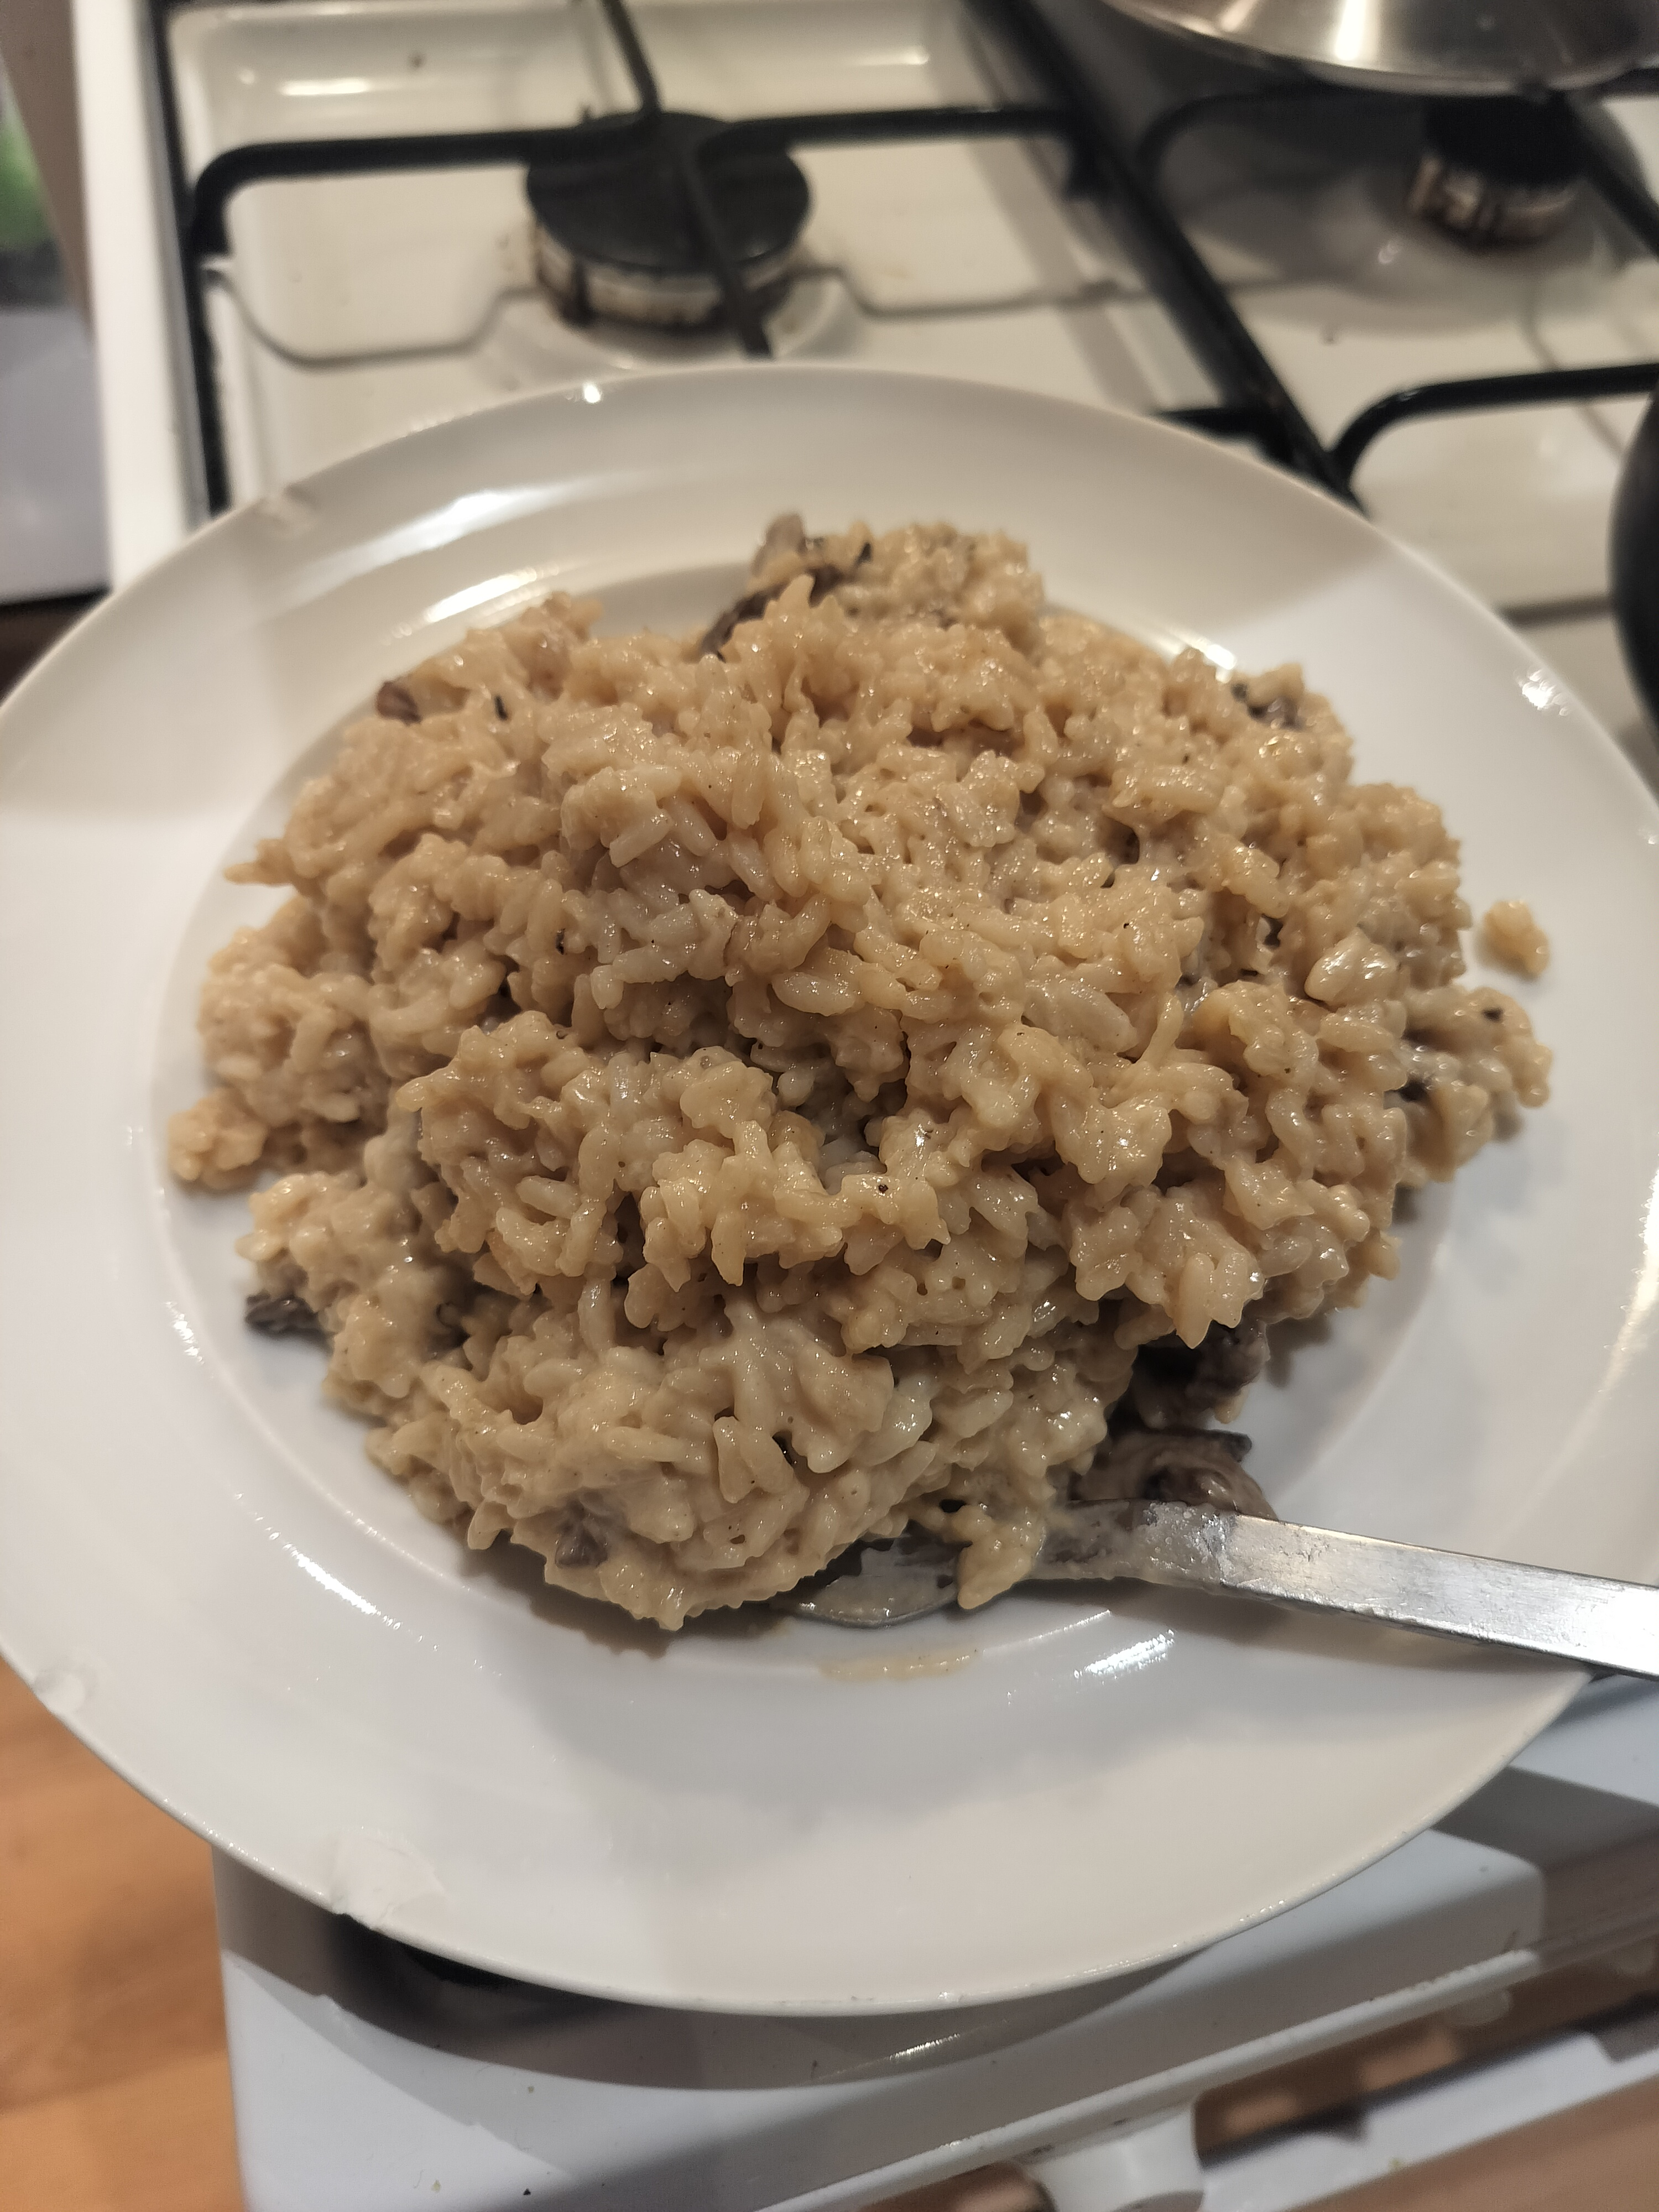
\includegraphics[width=\paperwidth,height=\paperheight]{Billeder/Aftensmad/Risotto.jpg}
    };
\end{tikzpicture}

%Her skulle der helst også være et billede, men istedet for tager vi et billede af mig på ski i Italien
%\begin{figure}
%    \centering
%   \includegraphics[width=0.5\linewidth]{Ski.jpg}
%    \caption{Ski tur i italien}
%\end{figure}
\newpage \section{Risotto Pasta}
\begin{minipage}[t]{0.5\textwidth}
\textbf{Ingredienser}
\begin{itemize}
    \item 2 løg, finthakket
    \item 3 fed hvidløg, presset
    \item 2 spsk olivenolie
    \item 1 grøntsagsbouillonterning
    \item svampe
    \begin{itemize}
        \item 250 g champignoner 
        \item 100 g Porto Bello svampe (kan undladdes)
        \item 50g kanteraller (kan undladdes)
    \end{itemize}
    \item 50g parmassen
    \item 2.5 dL fløde
    \item 250g frisk pasta
    \item Kryderrier
    \begin{itemize}
        \item 1 tsk timian
        \item kantarellfond
        \item salt og pebber
    \end{itemize}
\end{itemize}
\end{minipage}
\begin{minipage}[t]{0.5\textwidth}
\textbf{Fremgangsmåde:}
\begin{enumerate}
    \item Svits løgne i olie.
    \item Tilsæt de hakkedesvampe, og steg til blødet
    \item Tilsæt den firske pasta, boullionterningen, og vand nok til at dække pastaen.
    \item Når pastaen har fået den rette konsistens, skal noget af vandet hælles fra, og fløden og osten tilsættes.
\end{enumerate}
\end{minipage}
Til denne opskrift er det vigtigste at man har svampe i, kanatereller tilføje en hel masse lækker smag, men er ikke altid så let at få fat i, overordnet set vil jeg putte flere svampe i end men umiddelbart skulle tro, men elsker også svampe.
\newpage \begin{tikzpicture}[remember picture,overlay,inner sep=0pt,outer sep=0pt]
    \node[anchor=south east] at (current page.south east) {
        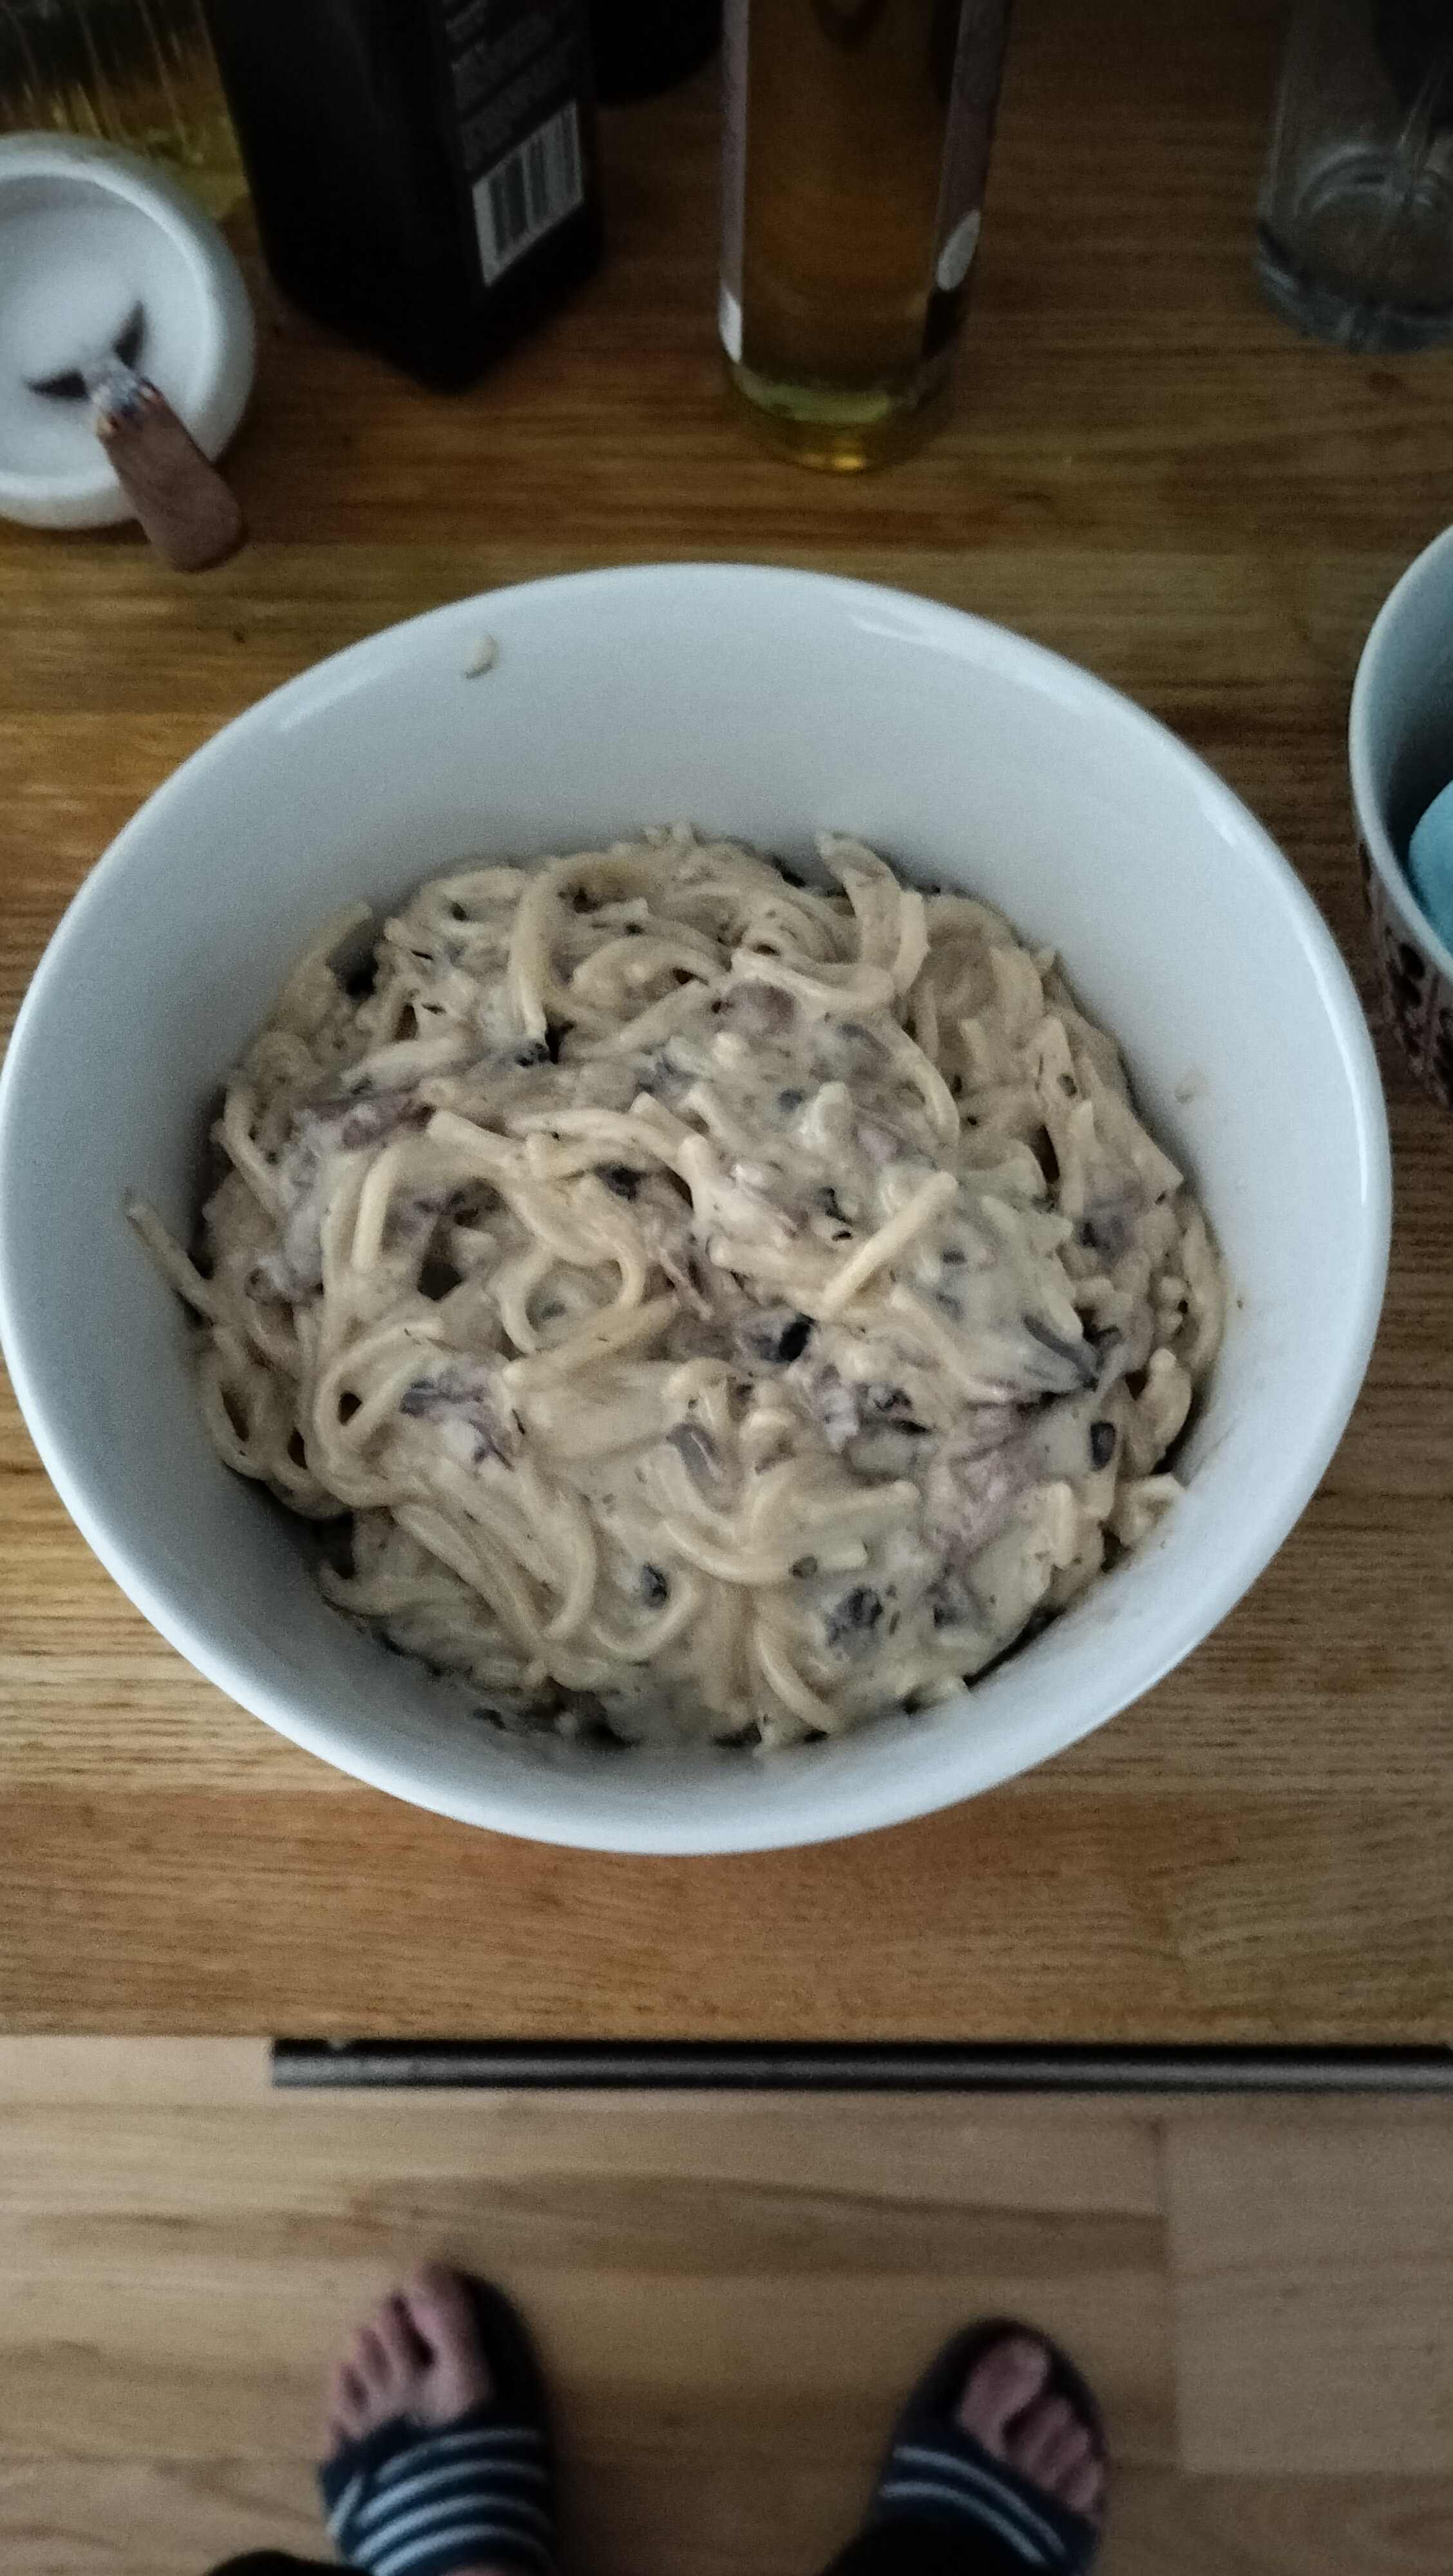
\includegraphics[width=\paperwidth,height=\paperheight]{Billeder/Aftensmad/PAstotto.jpg}
    };
\end{tikzpicture}
\newpage \section{Udon Nudel Suppe}
\begin{minipage}[t]{0.5\textwidth}
\textbf{Ingredienser:}
\begin{enumerate}
    \item 200g udon nudler
    \item 2 æg, hårdkogte
    \item 1-2 forårsløg, skåret i ringe
    \item 75 g champignoner, skiveskåret stege
    \item 50 g gulerødder, skiveskåret 
    \item 0.5 L grøntsagsbouillon 
    \item evt.
    \begin{itemize}
        \item Bønnespirer til topping
        \item Majs
        \item Ærter
        \item Mukimmame bønner
    \end{itemize}
\end{enumerate}
\end{minipage}
\begin{minipage}[t]{0.5\textwidth}
\textbf{Fremgangsmåde:}
\begin{enumerate}
    \item Klargør ingrediesnerne.
    \item Kog udon nudlerne i grøntsagsbouillon, sammen med de skiveskåret gullerøder.
    \item Pil æggene og server i halve , oven på nudelsuppen sammen med forårsløgne, champignoner og de andet ønsket topping.  
\end{enumerate}
\end{minipage}
Opskriften kan let opskaleres, og dette er bare nogel forslag på hvilke grøntsagerne der kunne være lækre i, generelt vil jeg foreslå grøntsager som er "friske" i smagen, som også ses i eventuelt.
\newpage \begin{tikzpicture}[remember picture,overlay,inner sep=0pt,outer sep=0pt]
    \node[anchor=south east] at (current page.south east) {
        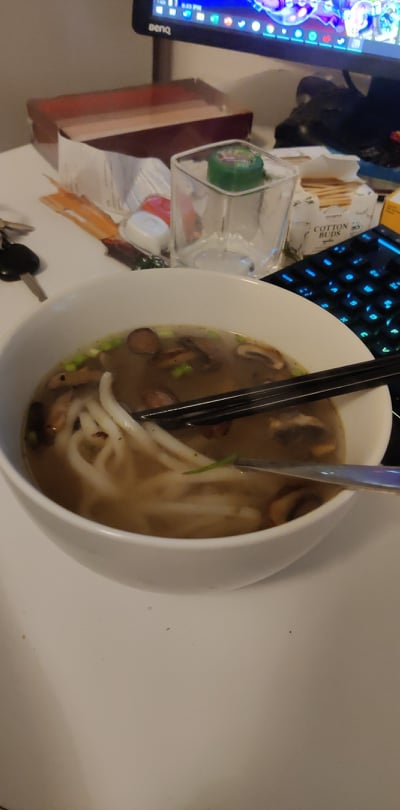
\includegraphics[width=\paperwidth,height=\paperheight]{Billeder/Aftensmad/Udon_nudel_Suppe.jpeg}
    };
\end{tikzpicture}
\chapter{Tilbehør}
\minitoc
\newpage \section{Bønnepasta}
\begin{minipage}[t]{0.5\textwidth}
\textbf{Ingredienser}
\begin{itemize}
    \item 2 mellemstore løg finthakket
    \item 1-2 fed hvidløg presset
    \item 1 dåse sortebønner
    \item 1 tsk tomatpasta
    \item Evt. 1 dåse hakkede tomatter
    \item krydderier
    \begin{itemize}
        \item 2 tsk Papriaka
        \item 1 tsk Chiliflager
        \item 1 tsk Cayennepeber
        \item 0.5 tsk stødt spidskommen
        \item salt og pebber
    \end{itemize}
\end{itemize}
\end{minipage}
\begin{minipage}[t]{0.5\textwidth}
\textbf{Fremgangsmåde:}
\begin{enumerate}
    \item Svits løgne i en kaserolle sammen med krydderierne.
    \item Tilsæt de sorte bønner og steg under log i omtrent 5 minutter
    \item Tilsæt tomatpastaen og eventuelt de hakkede tomatter, og kog op.
\end{enumerate}
\end{minipage}
De hakkede tomatter er eventuelt da det har en stor effekt på konsistensen, men kan anbefalle begge dele.
\newpage 
Her skulle der jo sjovt nok være et billede af nogle bønner, istedet for tager vi et billede af dragen Helmut 
\begin{figure}
    \centering
    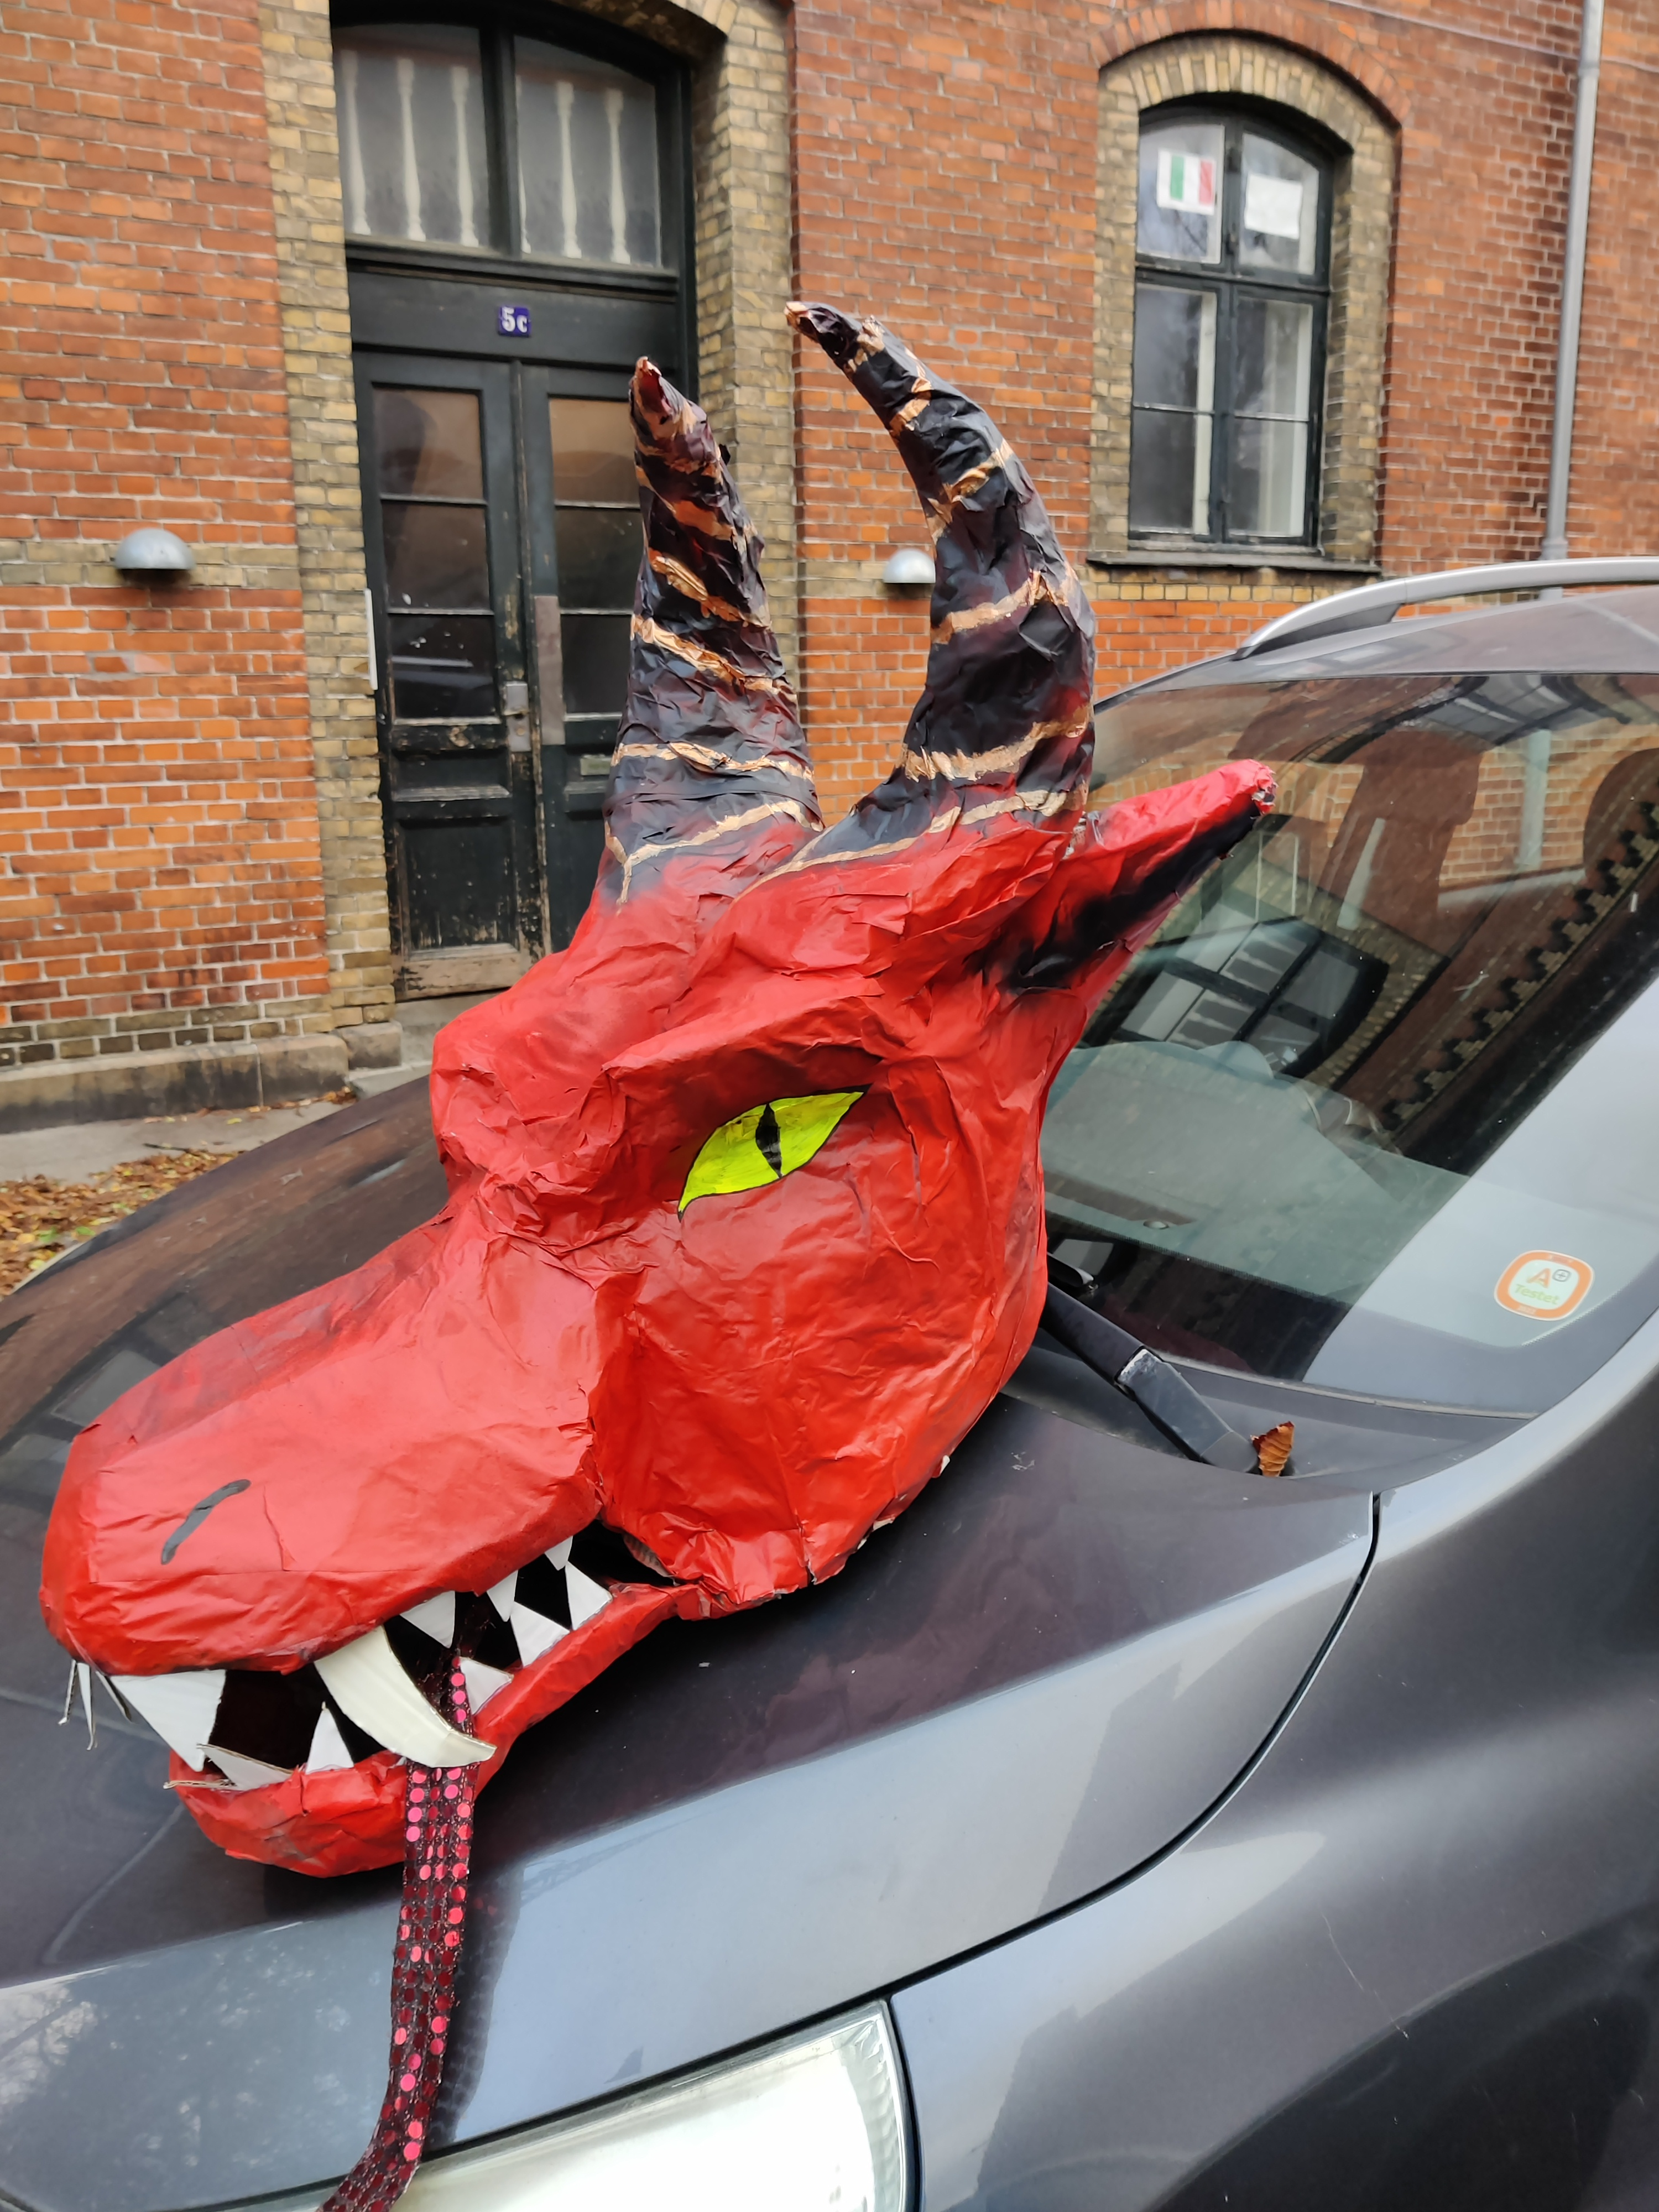
\includegraphics[width=0.5\linewidth]{Helmut.jpg}
    \caption{Dragen helmut}
  
\end{figure}
\newpage \section{Græsk Yoghurt Dressing}
\begin{minipage}[t]{0.5\textwidth}
\textbf{Ingredienser:}
 \begin{enumerate}
        \item 200g græsk yoghurt 
        \item 2 tsk stødt spiskommen
        \item 1 tsk stødt korander
        \item Salt og pebber
    \end{enumerate}
\end{minipage}
\begin{minipage}[t]{0.5\textwidth}
\textbf{Fremgangsmåde:}
\begin{enumerate}
    \item Miks alle ingredienser til krydderierne er ligelig fordelt.
\end{enumerate}
\end{minipage}
\newpage 
\begin{tikzpicture}[remember picture,overlay,inner sep=0pt,outer sep=0pt]
    \node[anchor=south east] at (current page.south east) {
        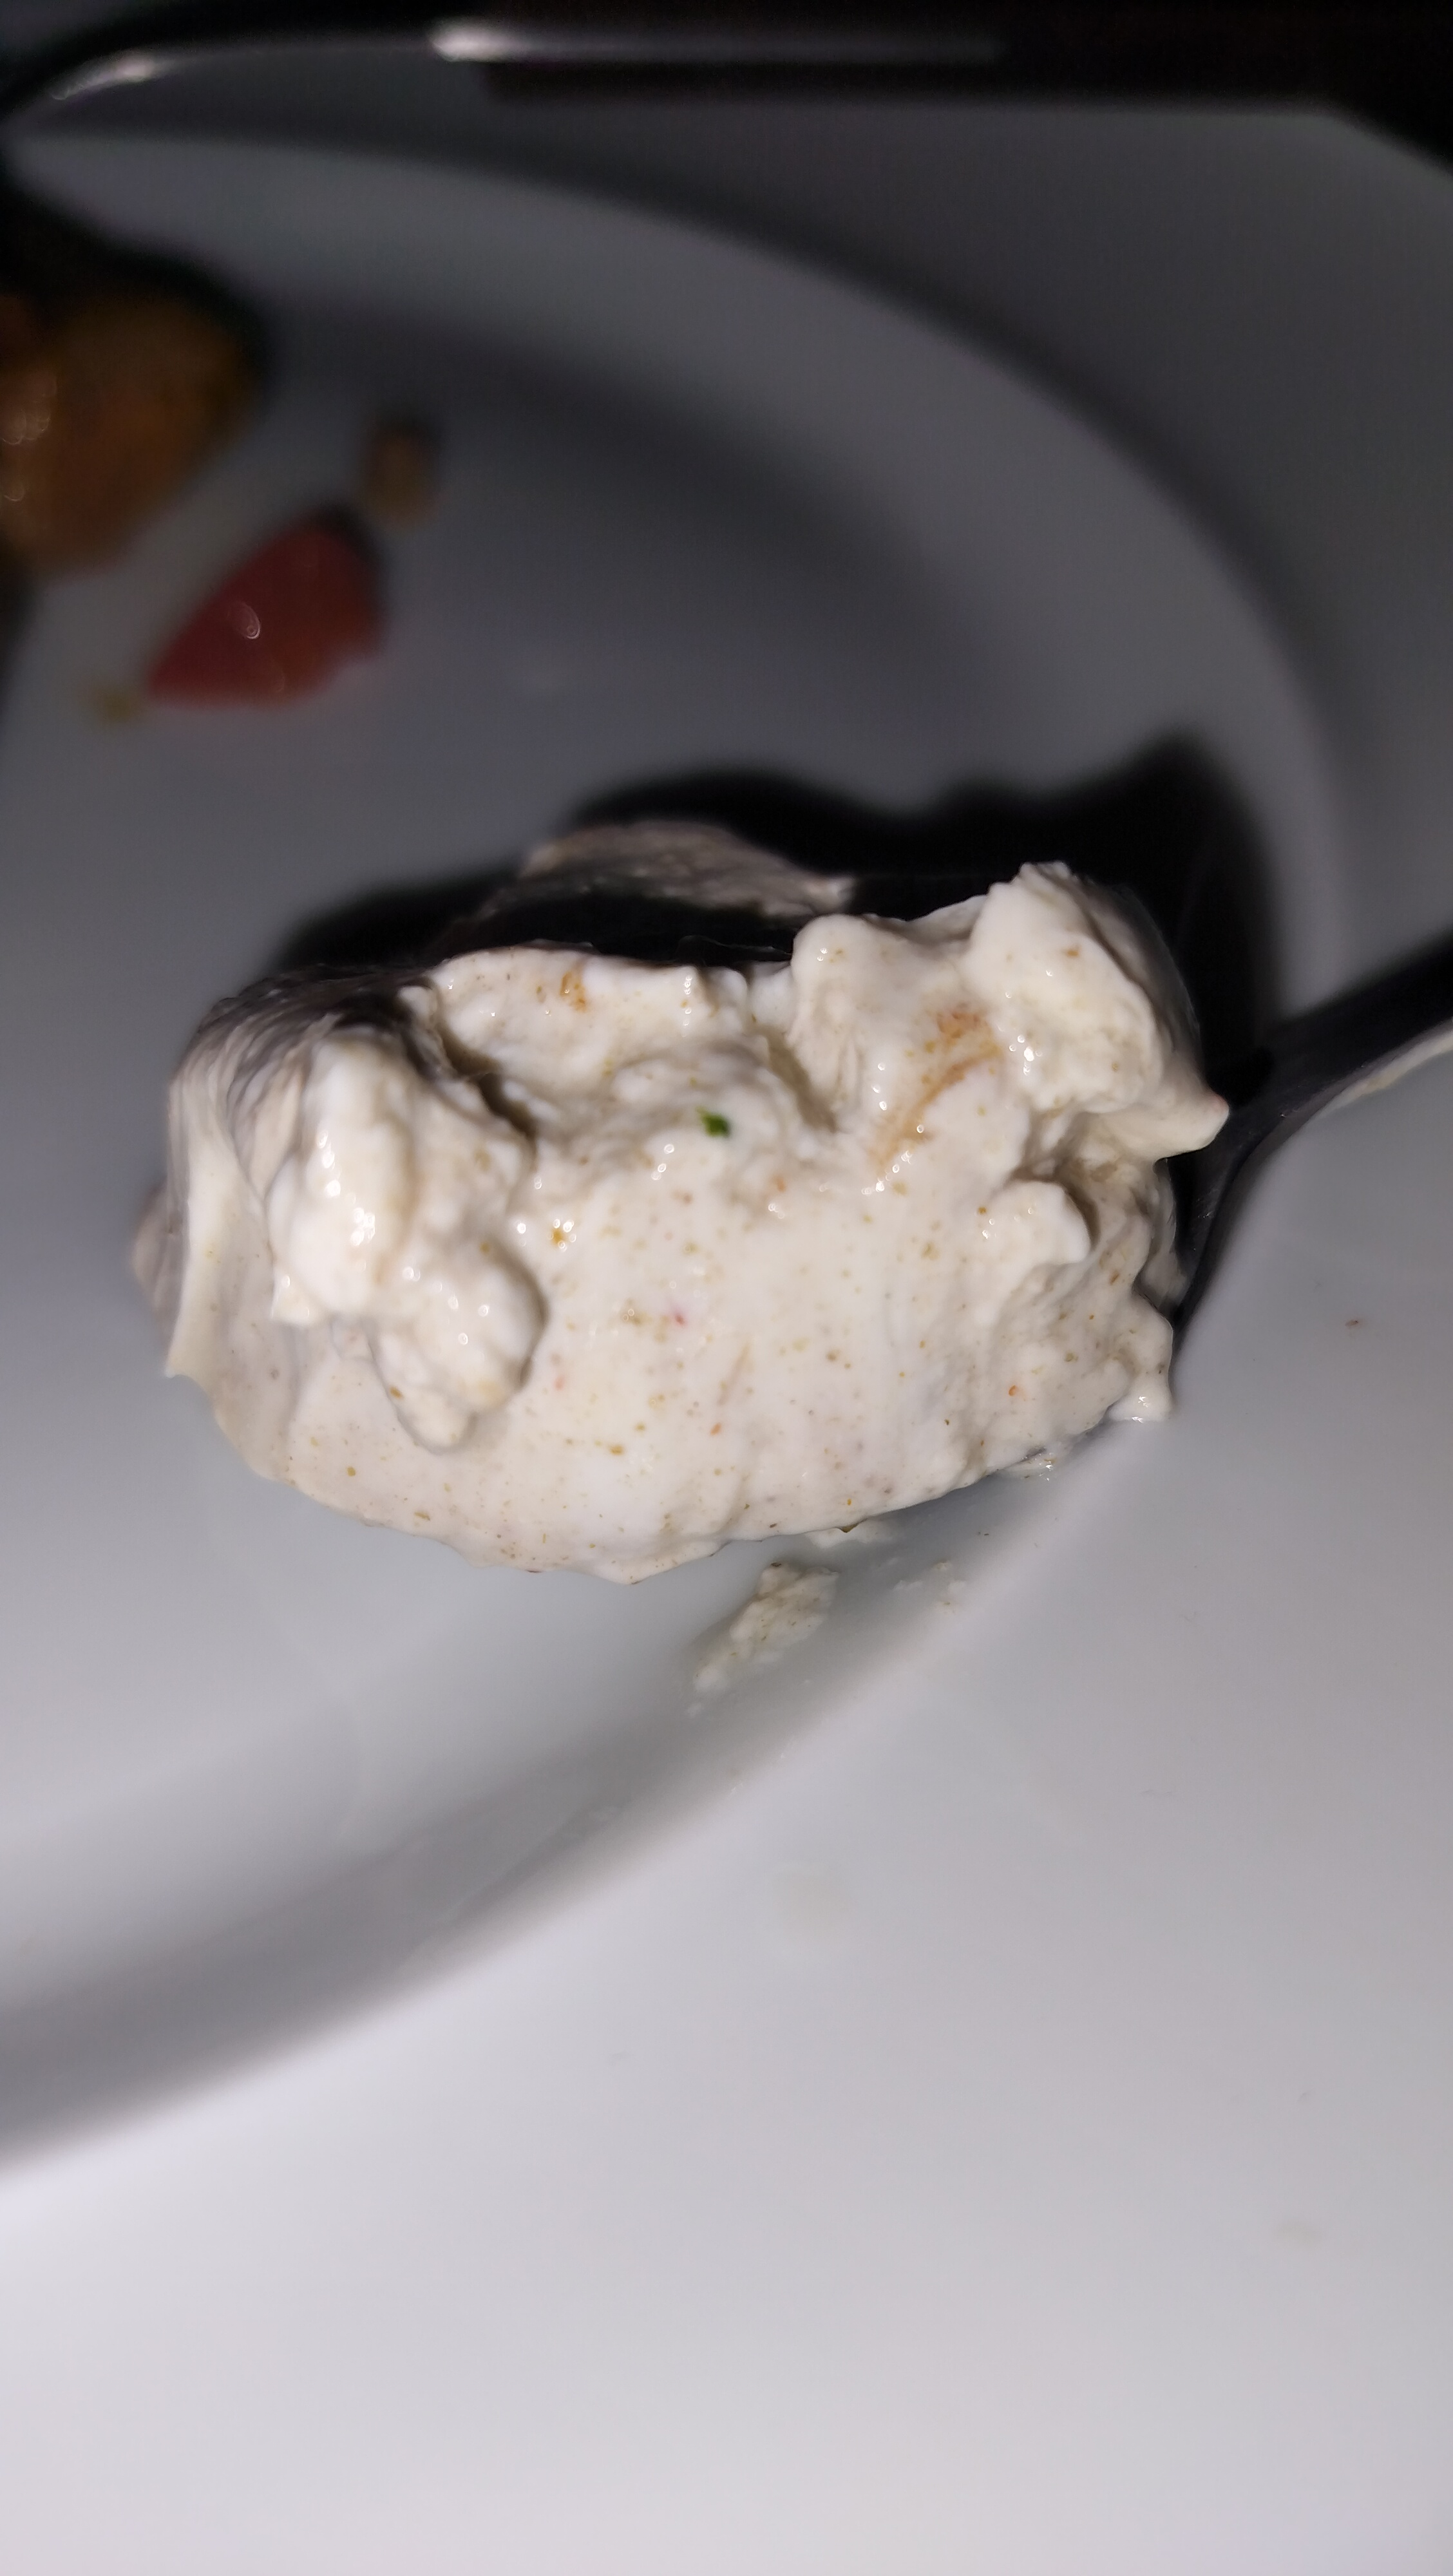
\includegraphics[width=\paperwidth,height=\paperheight]{Billeder/Tilbehør/Græsk_Yoghurt_Dressing.jpg}
    };
\end{tikzpicture}
\newpage \section{Hummus}
\begin{minipage}[t]{0.5\textwidth}
\textbf{Ingredienser:}
\begin{itemize}
    \item 1 dåse kikærter
    \item 1 spsk tahin eller smooth peanutbutter
    \item Citronsaft efter ønske
    \item Mindst 2 fed hvidlæg
    \item 1 tsk stødt spidskommen
    \item En smule cayenne peber
    \item 0.5 dL kold vand (alt efter konsitens)
    \item 3 spsk olivenolie
    \item En smule salt (tahin er meget saltet i sig selv)
    \item Peber
    \item Smag varians
    \begin{enumerate}
        \item evt. soltørret tomatter
        \item evt. oliven og kapres
        \item evt. rødbedder
        \item evt. avocaddo
    \end{enumerate}
\end{itemize}
\end{minipage}
\begin{minipage}[t]{0.5\textwidth}
\textbf{Fremgangsmåde}
\begin{enumerate}
    \item Bland alt sammen minus vand og blend i food processor, tilsæt til sidst vand alt efter konsitens.
    \item Hummus kan med fordel laves med forskellige smage ved at dele hummus portionen i flere portioner og blendt de ønskede smage sammen med hummusen.  
\end{enumerate}
\end{minipage}
Som udganspunkt er Peanut butter en 1:1 erstatning af tahinn, dog er det ikke helt lige så saltet, og giver en svag jordnøde smag, dette synes jeg dog let overdøves af de soltørret tomatter eller en af de andre smags varinter. Smags varianterne skal ses som enten den ene eller den anden, mit forsøg på at lave en oliven tomat en, gav hvertfald bare rød oliven hummus.
\newpage
\begin{tikzpicture}[remember picture,overlay,inner sep=0pt,outer sep=0pt]
    \node[anchor=south east] at (current page.south east) {
        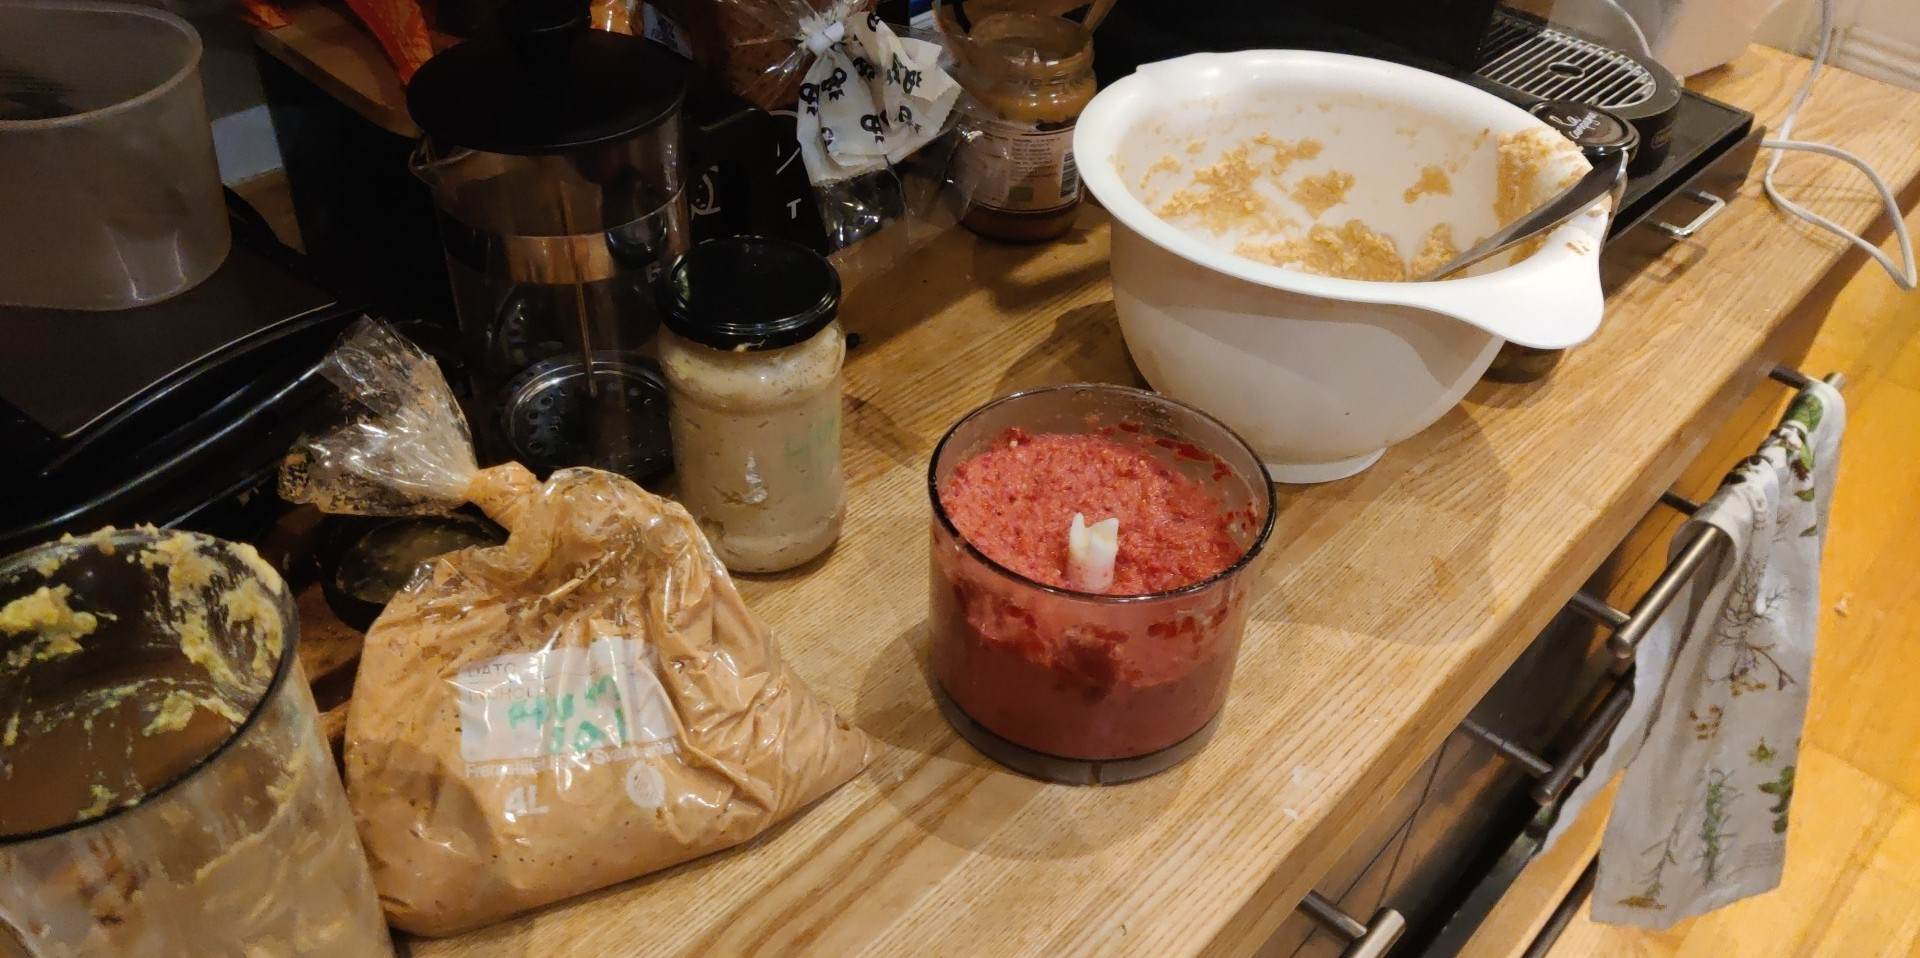
\includegraphics[width=\paperwidth,height=\paperheight]{Billeder/Tilbehør/Hummus.jpeg}
    };
\end{tikzpicture}
\newpage \section{Hvidløgssmør}
\begin{minipage}[t]{0.5\textwidth}
\textbf{Ingrediesner:}
\begin{itemize}
    \item 200 gram smør
    \item 4-5 fed hvidløg, hakket eller presset
\end{itemize}
\end{minipage}
\begin{minipage}[t]{0.5\textwidth}
\textbf{Fremgangsmåde:}
\begin{enumerate}
    \item Blød smøren til den er kan æltes
    \item Pres eller hak hvidløgne, og fordel så jævnligt  som muligt.
    \item Stil på køl til det skal bruges.
\end{enumerate}
\end{minipage}
Denne opskrift er relativ simpel men der er et par ting man skal være opmærksom på. SMører skal helst være blødt, man kan som udganspunnkt godt smelte smøret og tilføje hvidløgen, men dette giver en lidt underligt konsistens til hvidløgssmøren, vil dermed anbefale at man lader det stå ude i 20-30 minutter, og så mikser det enten med hænderne eller spise pinde. 
\newpage \begin{tikzpicture}[remember picture,overlay,inner sep=0pt,outer sep=0pt]
    \node[anchor=south east] at (current page.south east) {
        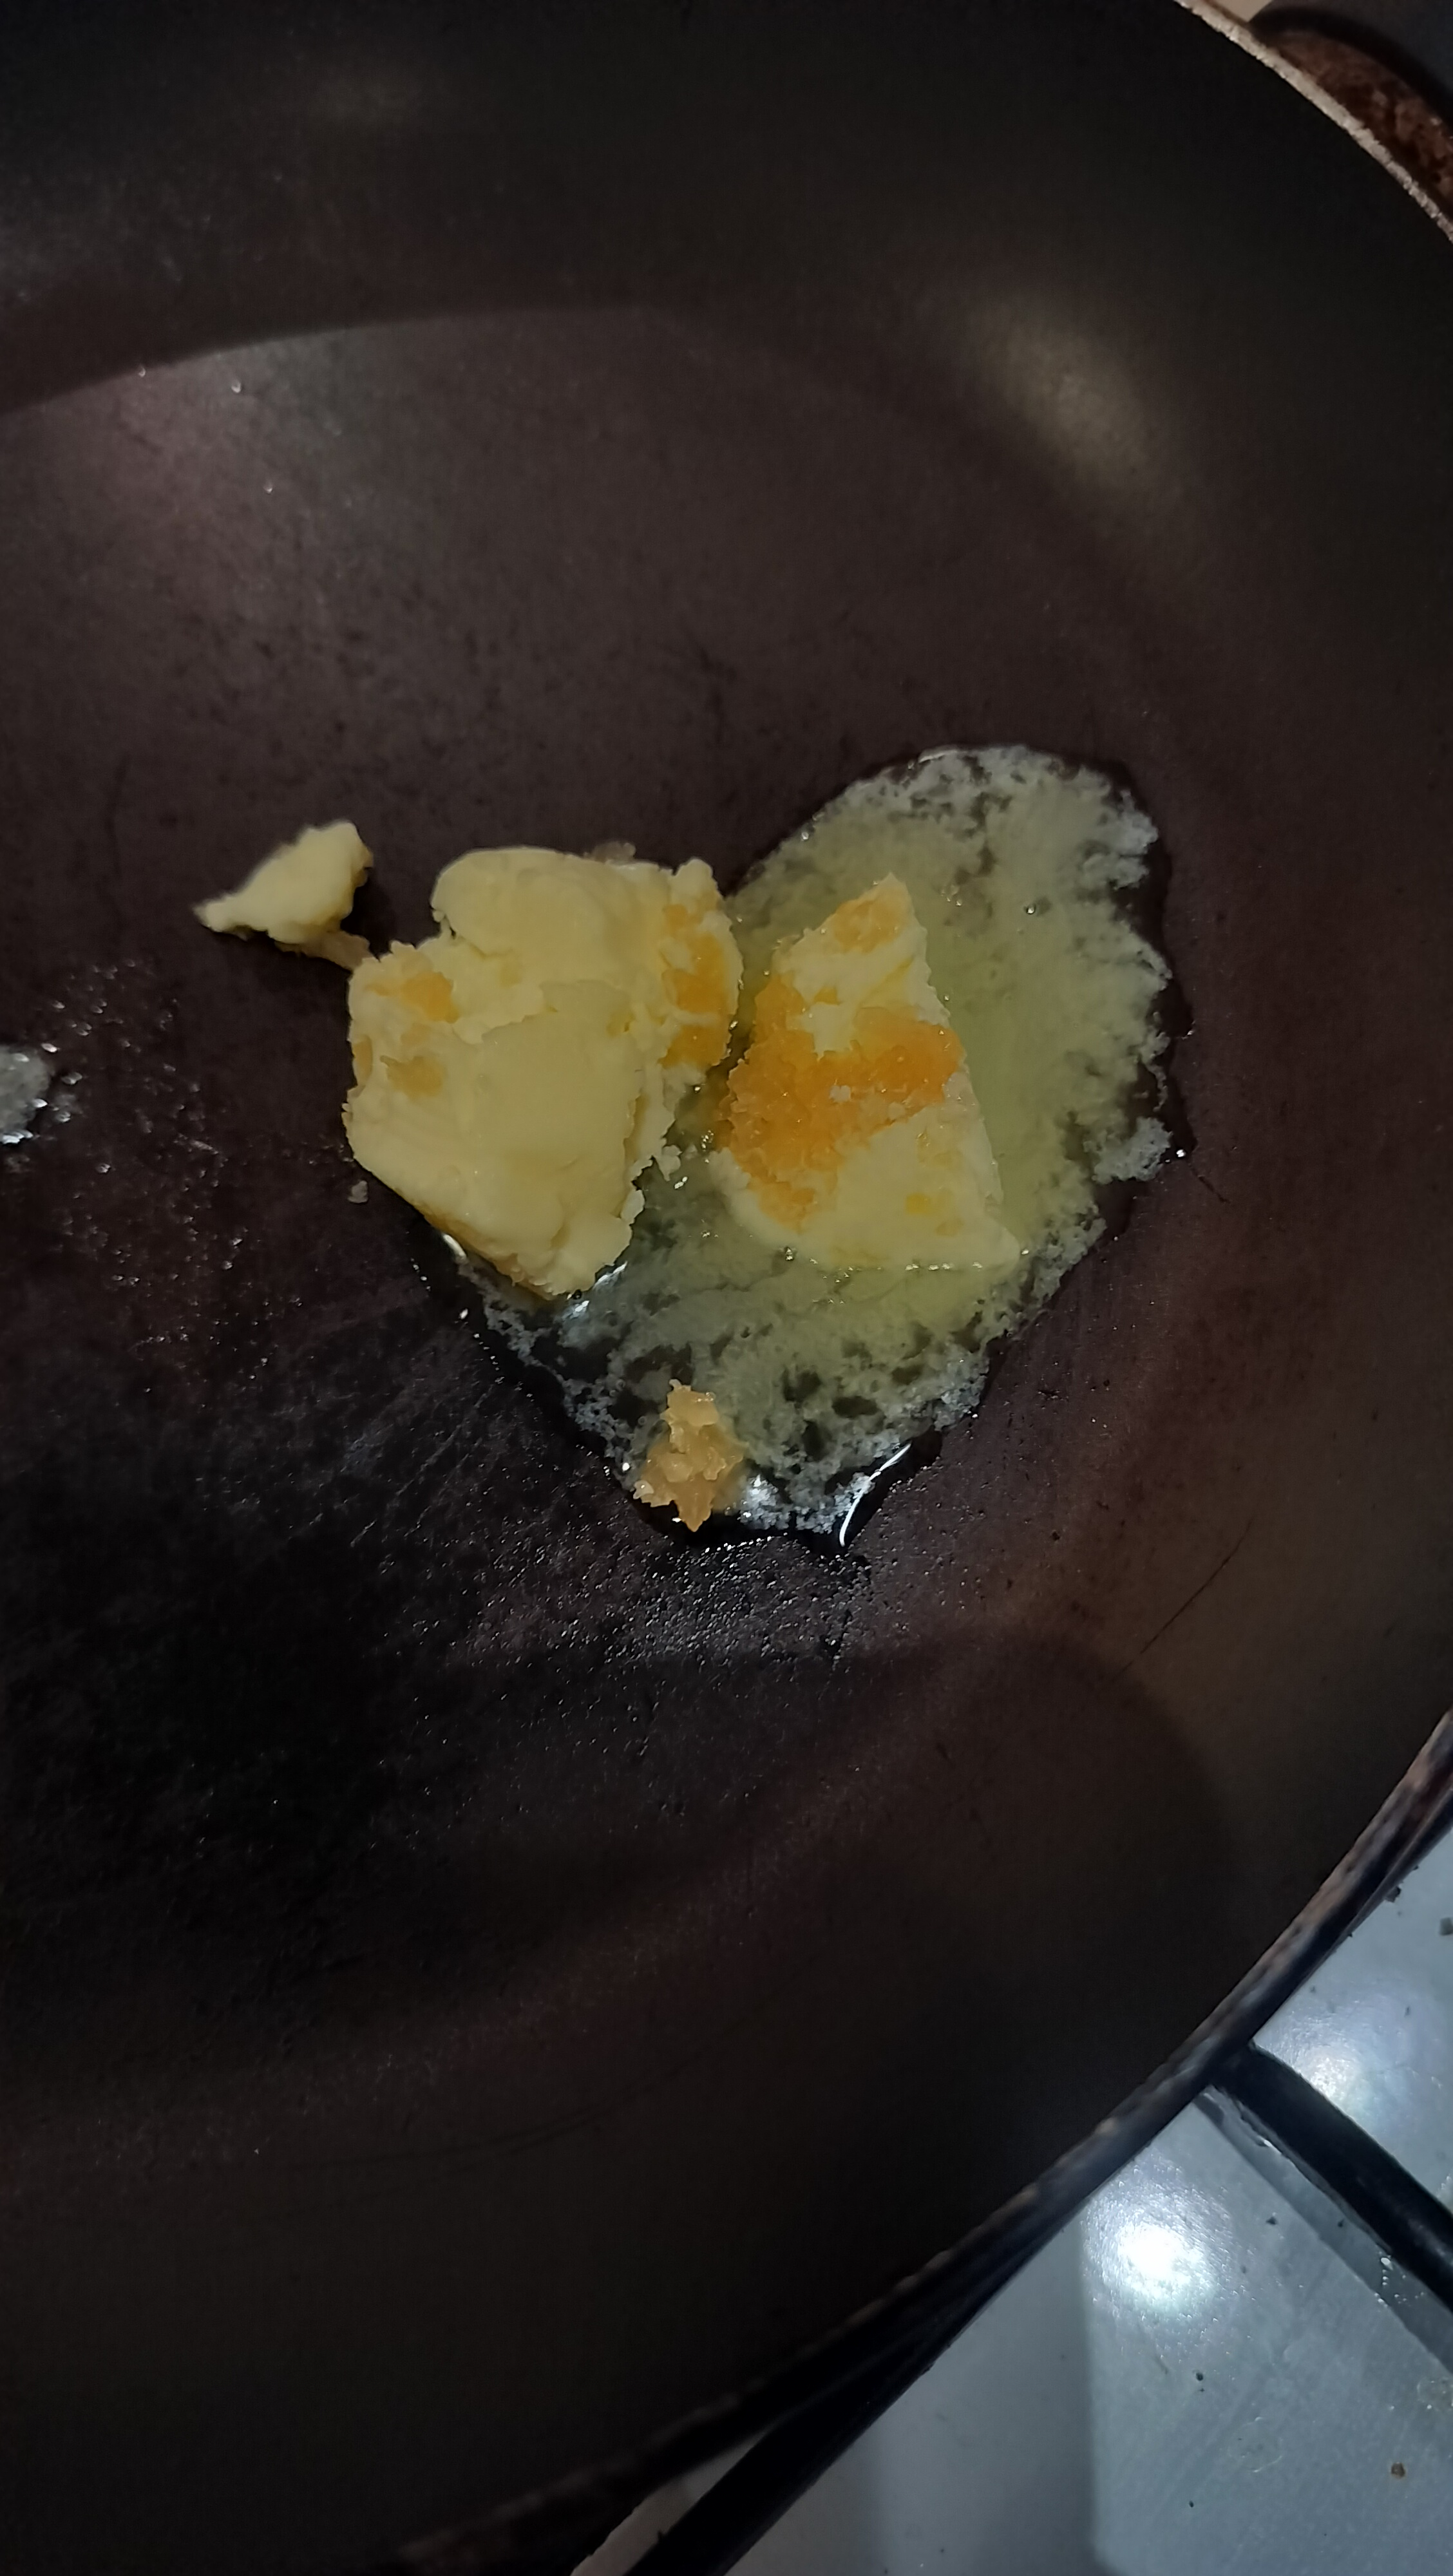
\includegraphics[width=\paperwidth,height=\paperheight]{Billeder/Tilbehør/Hvidløgssmør.jpg}
    };
\end{tikzpicture}
\newpage \section{Oliven Tapparnade}
\begin{minipage}[t]{0.5\textwidth}
\textbf{Ingredienser:}
\begin{itemize}
    \item 200g sorte oliven
    \item 2 spsk olivenolie
    \item kapers
    \item 3 fed hvidløg
\end{itemize}
\end{minipage}
\begin{minipage}[t]{0.5\textwidth}
\begin{enumerate}
    \item Tilsæt alle ingredienserne og blend i food processor til ønskede konsitens
\end{enumerate}
\end{minipage}
Jeg synes personligt at det er lækkert når olivener er i små stykker, men stadig mere individuelt.
\newpage Her skulle der så også være et billede, så vi tager en anden måge i Oslo
\begin{figure}
    \centering
    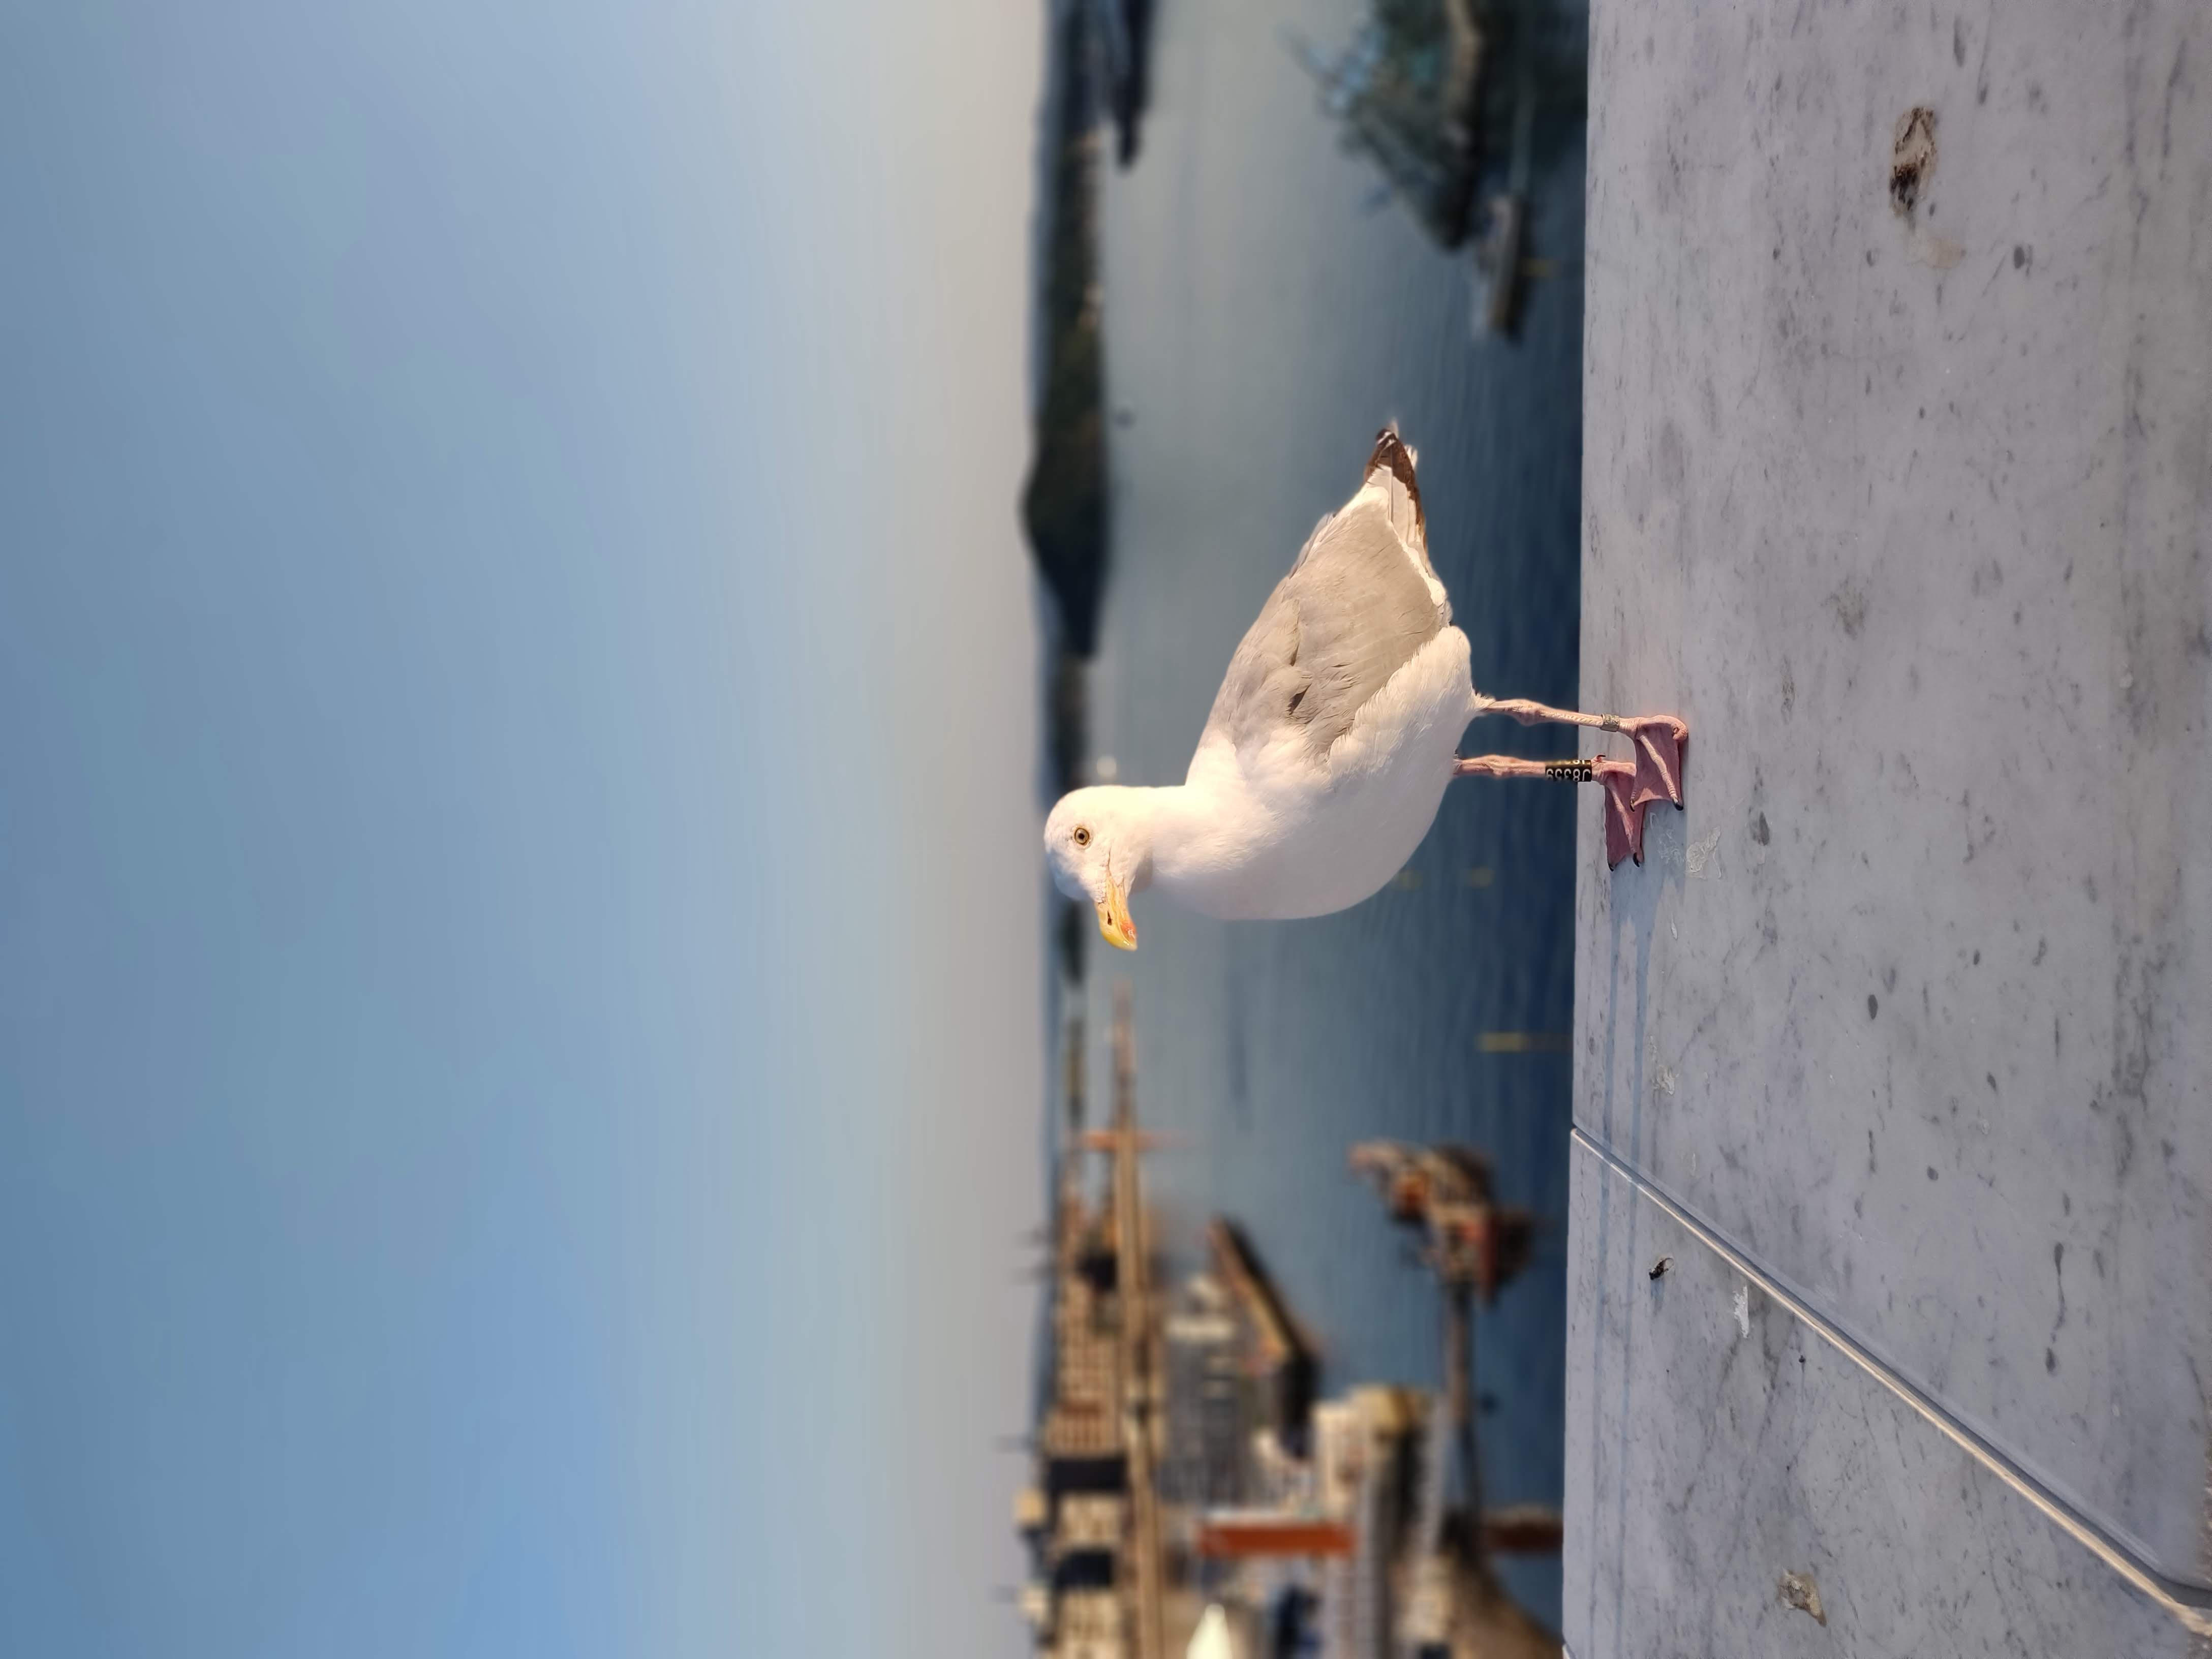
\includegraphics[width=0.5\linewidth]{Måge2.jpg}
    \caption{Måge nr 2}
    
\end{figure}
\newpage \section{Pico de Gallo}
\begin{minipage}[t]{0.5\textwidth}
\textbf{Ingredienser:}
\begin{itemize}
    \item 3-4 tomatter, skåret i tern
    \item 1-2 røde løg, skåret i tern
    \item 0.5 håndfuld friske koriander
    \item 1 fed hvidløg, presset
    \item Citron- eller lime-saft
    \item Salt og pebber
\end{itemize}
\end{minipage}
\begin{minipage}[t]{0.5\textwidth}
\begin{enumerate}
    \item Dræn tomatterne for noget af væden.
    \item Miks alle ingredienserne i en skål.
    \item Lad stå på køl i helst en time, gerne længere
\end{enumerate}
\end{minipage}
\newpage 
\begin{tikzpicture}[remember picture,overlay,inner sep=0pt,outer sep=0pt]
    \node[anchor=south east] at (current page.south east) {
        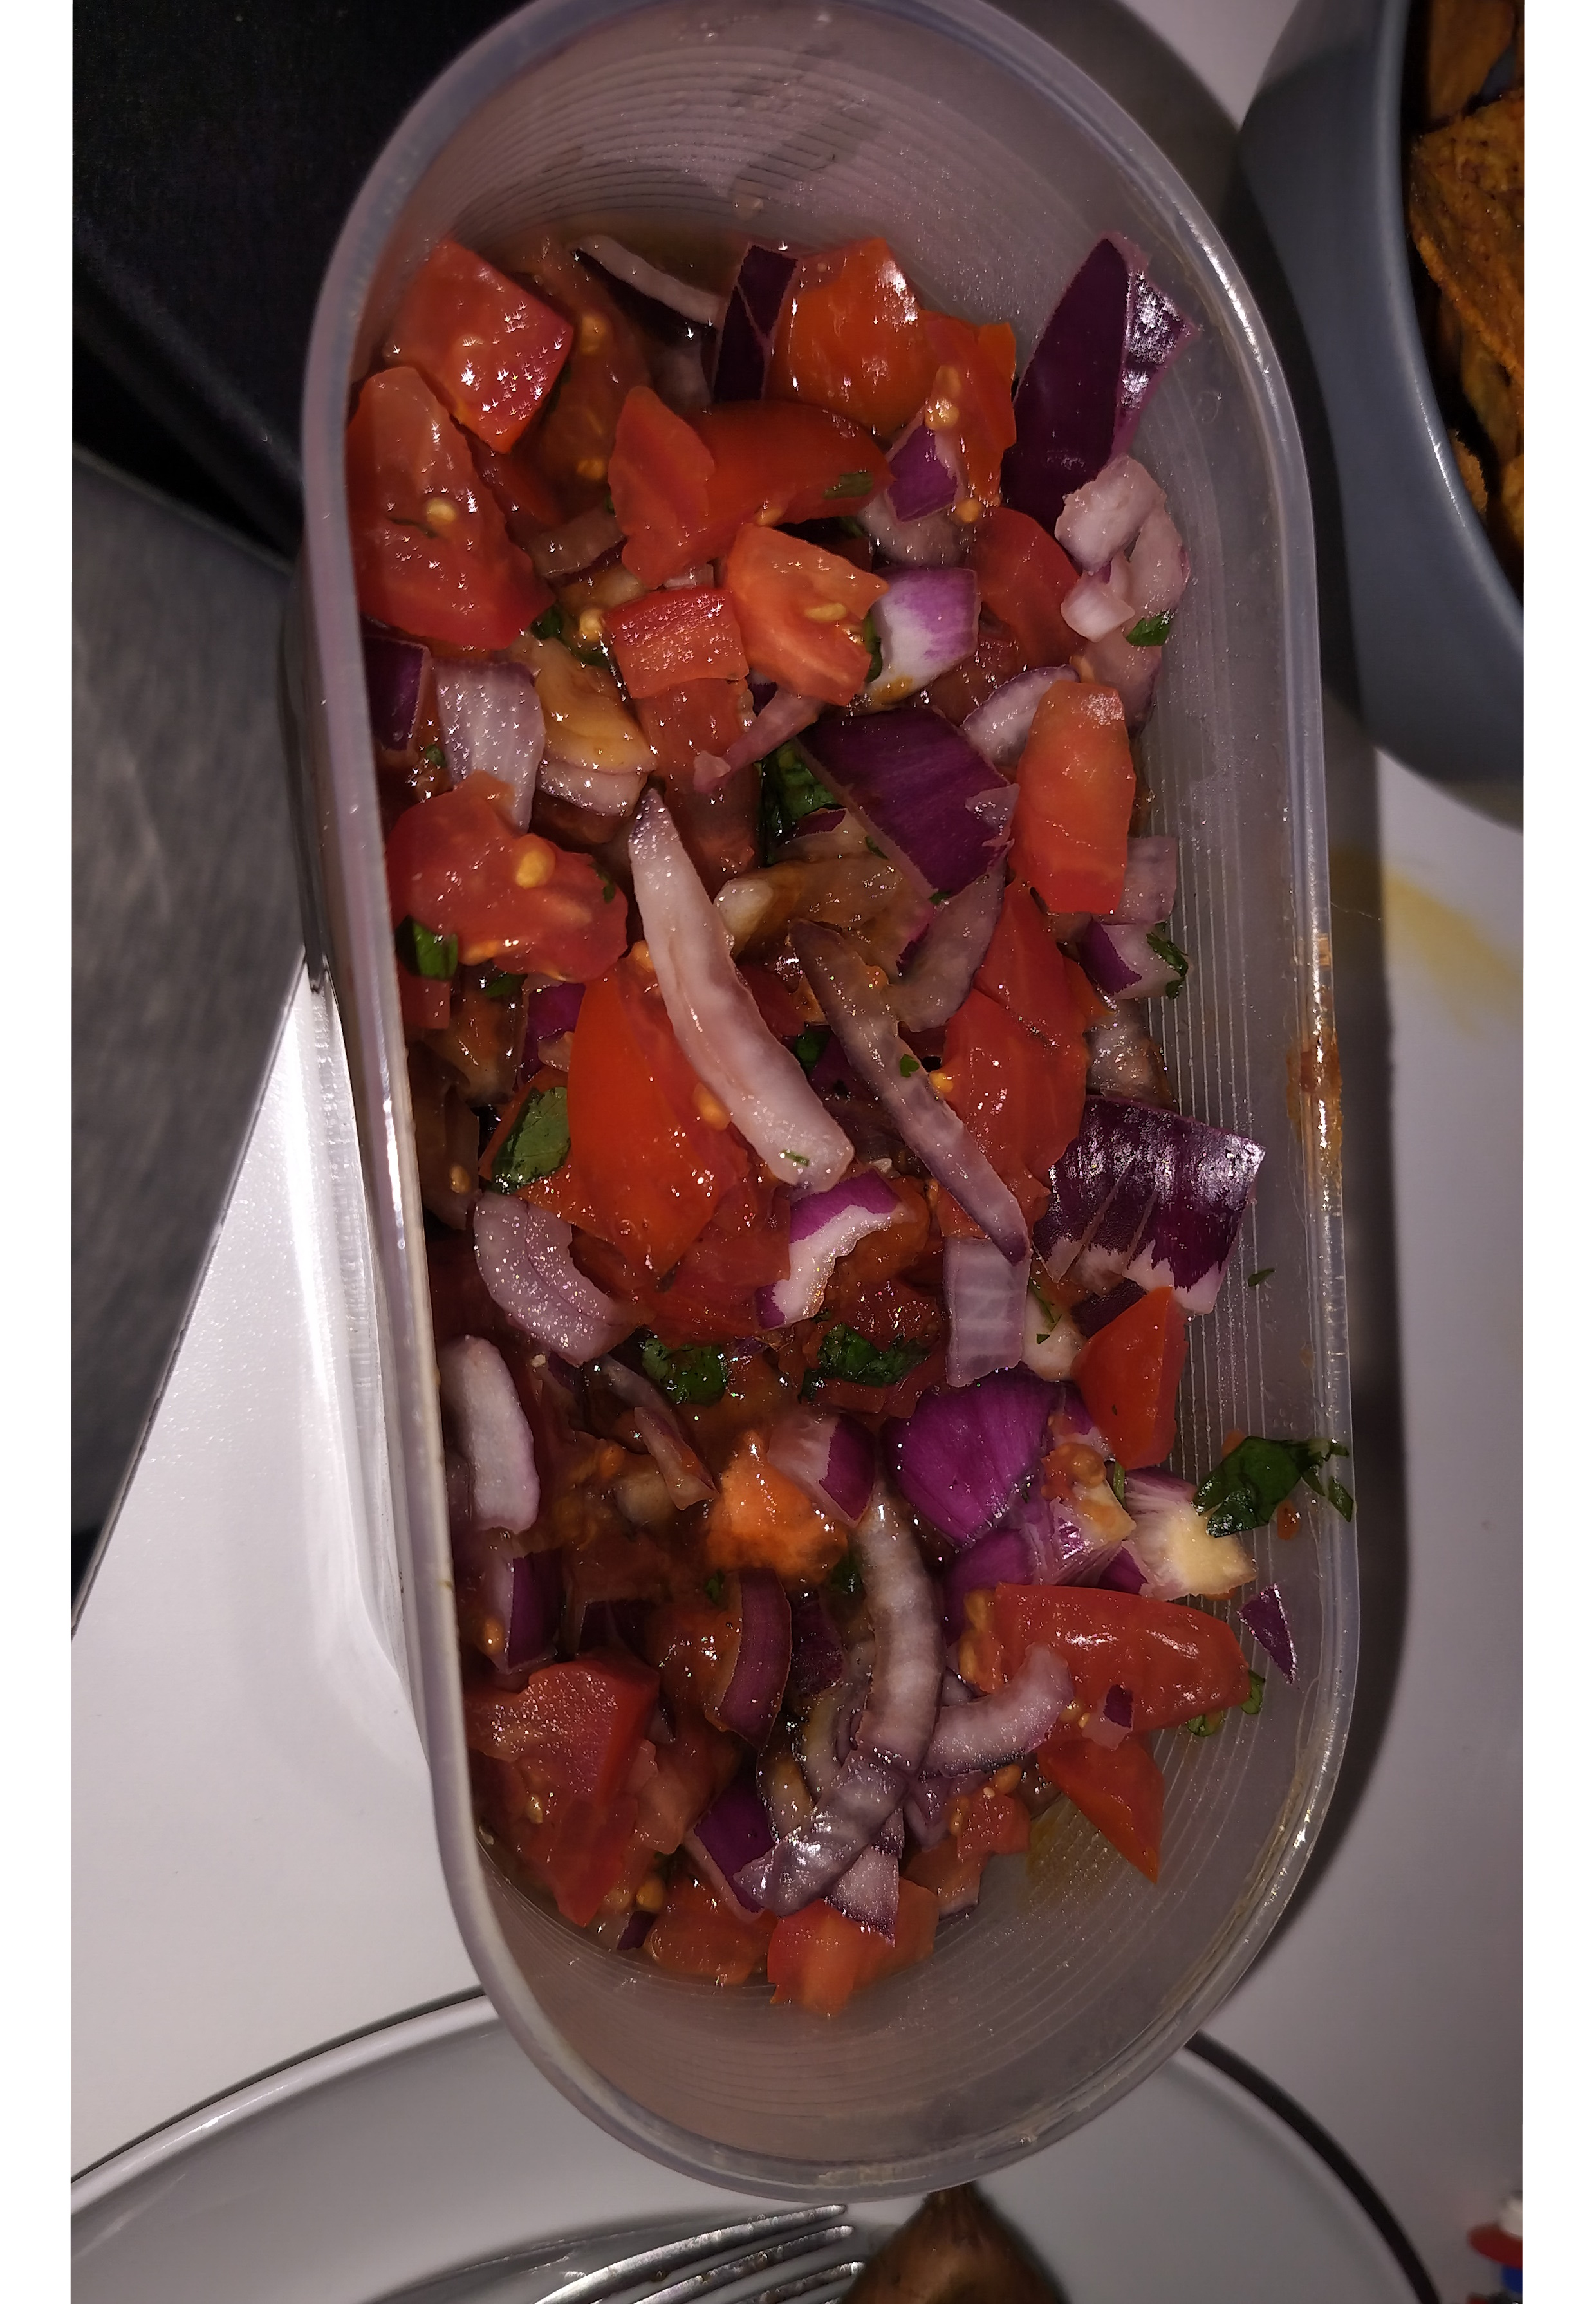
\includegraphics[width=\paperwidth,height=\paperheight]{Billeder/Tilbehør/Pico2.png}
    };
\end{tikzpicture}
\newpage\section{Porto Bello Svampe med Ost}
\begin{minipage}[t]{0.5\textwidth}
\textbf{Ingredienser:}
\begin{itemize}
    \item Porto Bello Svamp (helst releativ storre)
    \item En eller flere af de følgende ost
    \begin{enumerate}
        \item Gedeost
        \item Mozzarella kugle
        \item Blå ost
    \end{enumerate}
\end{itemize}
\end{minipage}
\begin{minipage}[t]{0.5\textwidth}
\begin{enumerate}
    \item Vask porto bello svampene, fjern  stilken og eventuel lamellerne
    \item Den fjernet stil og de evneutelle lameller kan skæres i stykke og blandes sammen med den ønskede ost
    \item Steg i ovnen eller på grillen til osten er smeltet (\~15 minutter ved 200 \degree C varmluft)
\end{enumerate}
\end{minipage}
Til denne opskrift er der ikke det store af mål, da det kommer and på hvor ostet man vil have det. Med mozerella kan en kugle med fordel bruges til 2-3 porto bello svampe.

\newpage \section{Svampe Suace}

\begin{minipage}[t]{0.5\textwidth}
\textbf{Ingredeisner:}
\begin{itemize}
    \item 2 spsk smør
    \item 1/2 spsk olivenolie
    \item 300 g champingioner hakket 
    \item 2-3 fed hvidløg, presset
    \item Et skvat hvidvin
    \item 125 mL grøntsagsboullon
    \item 50 g parmassen
    \item timian
    \item salt og peber
\end{itemize}
\end{minipage}
\begin{minipage}[t]{0.5\textwidth}
\textbf{Fremgangsmåde:}
\begin{enumerate}
    \item Smeltsmøren og varm olien i en gryde sammen med svampene ved høj varme.
    \item Når de er blødt tilsæt hvidløget.
    \item Hæl vinen i under omrøring.
    \item Tilsæt grøntsagsboulliounen, fløden og parmassaen, og skru ned for varmen.
    \item Rør i 2-3 minutter, og smag til med timian, salt og peber.
\end{enumerate}
\end{minipage}
\newpage \begin{tikzpicture}[remember picture,overlay,inner sep=0pt,outer sep=0pt]
    \node[anchor=south east] at (current page.south east) {
        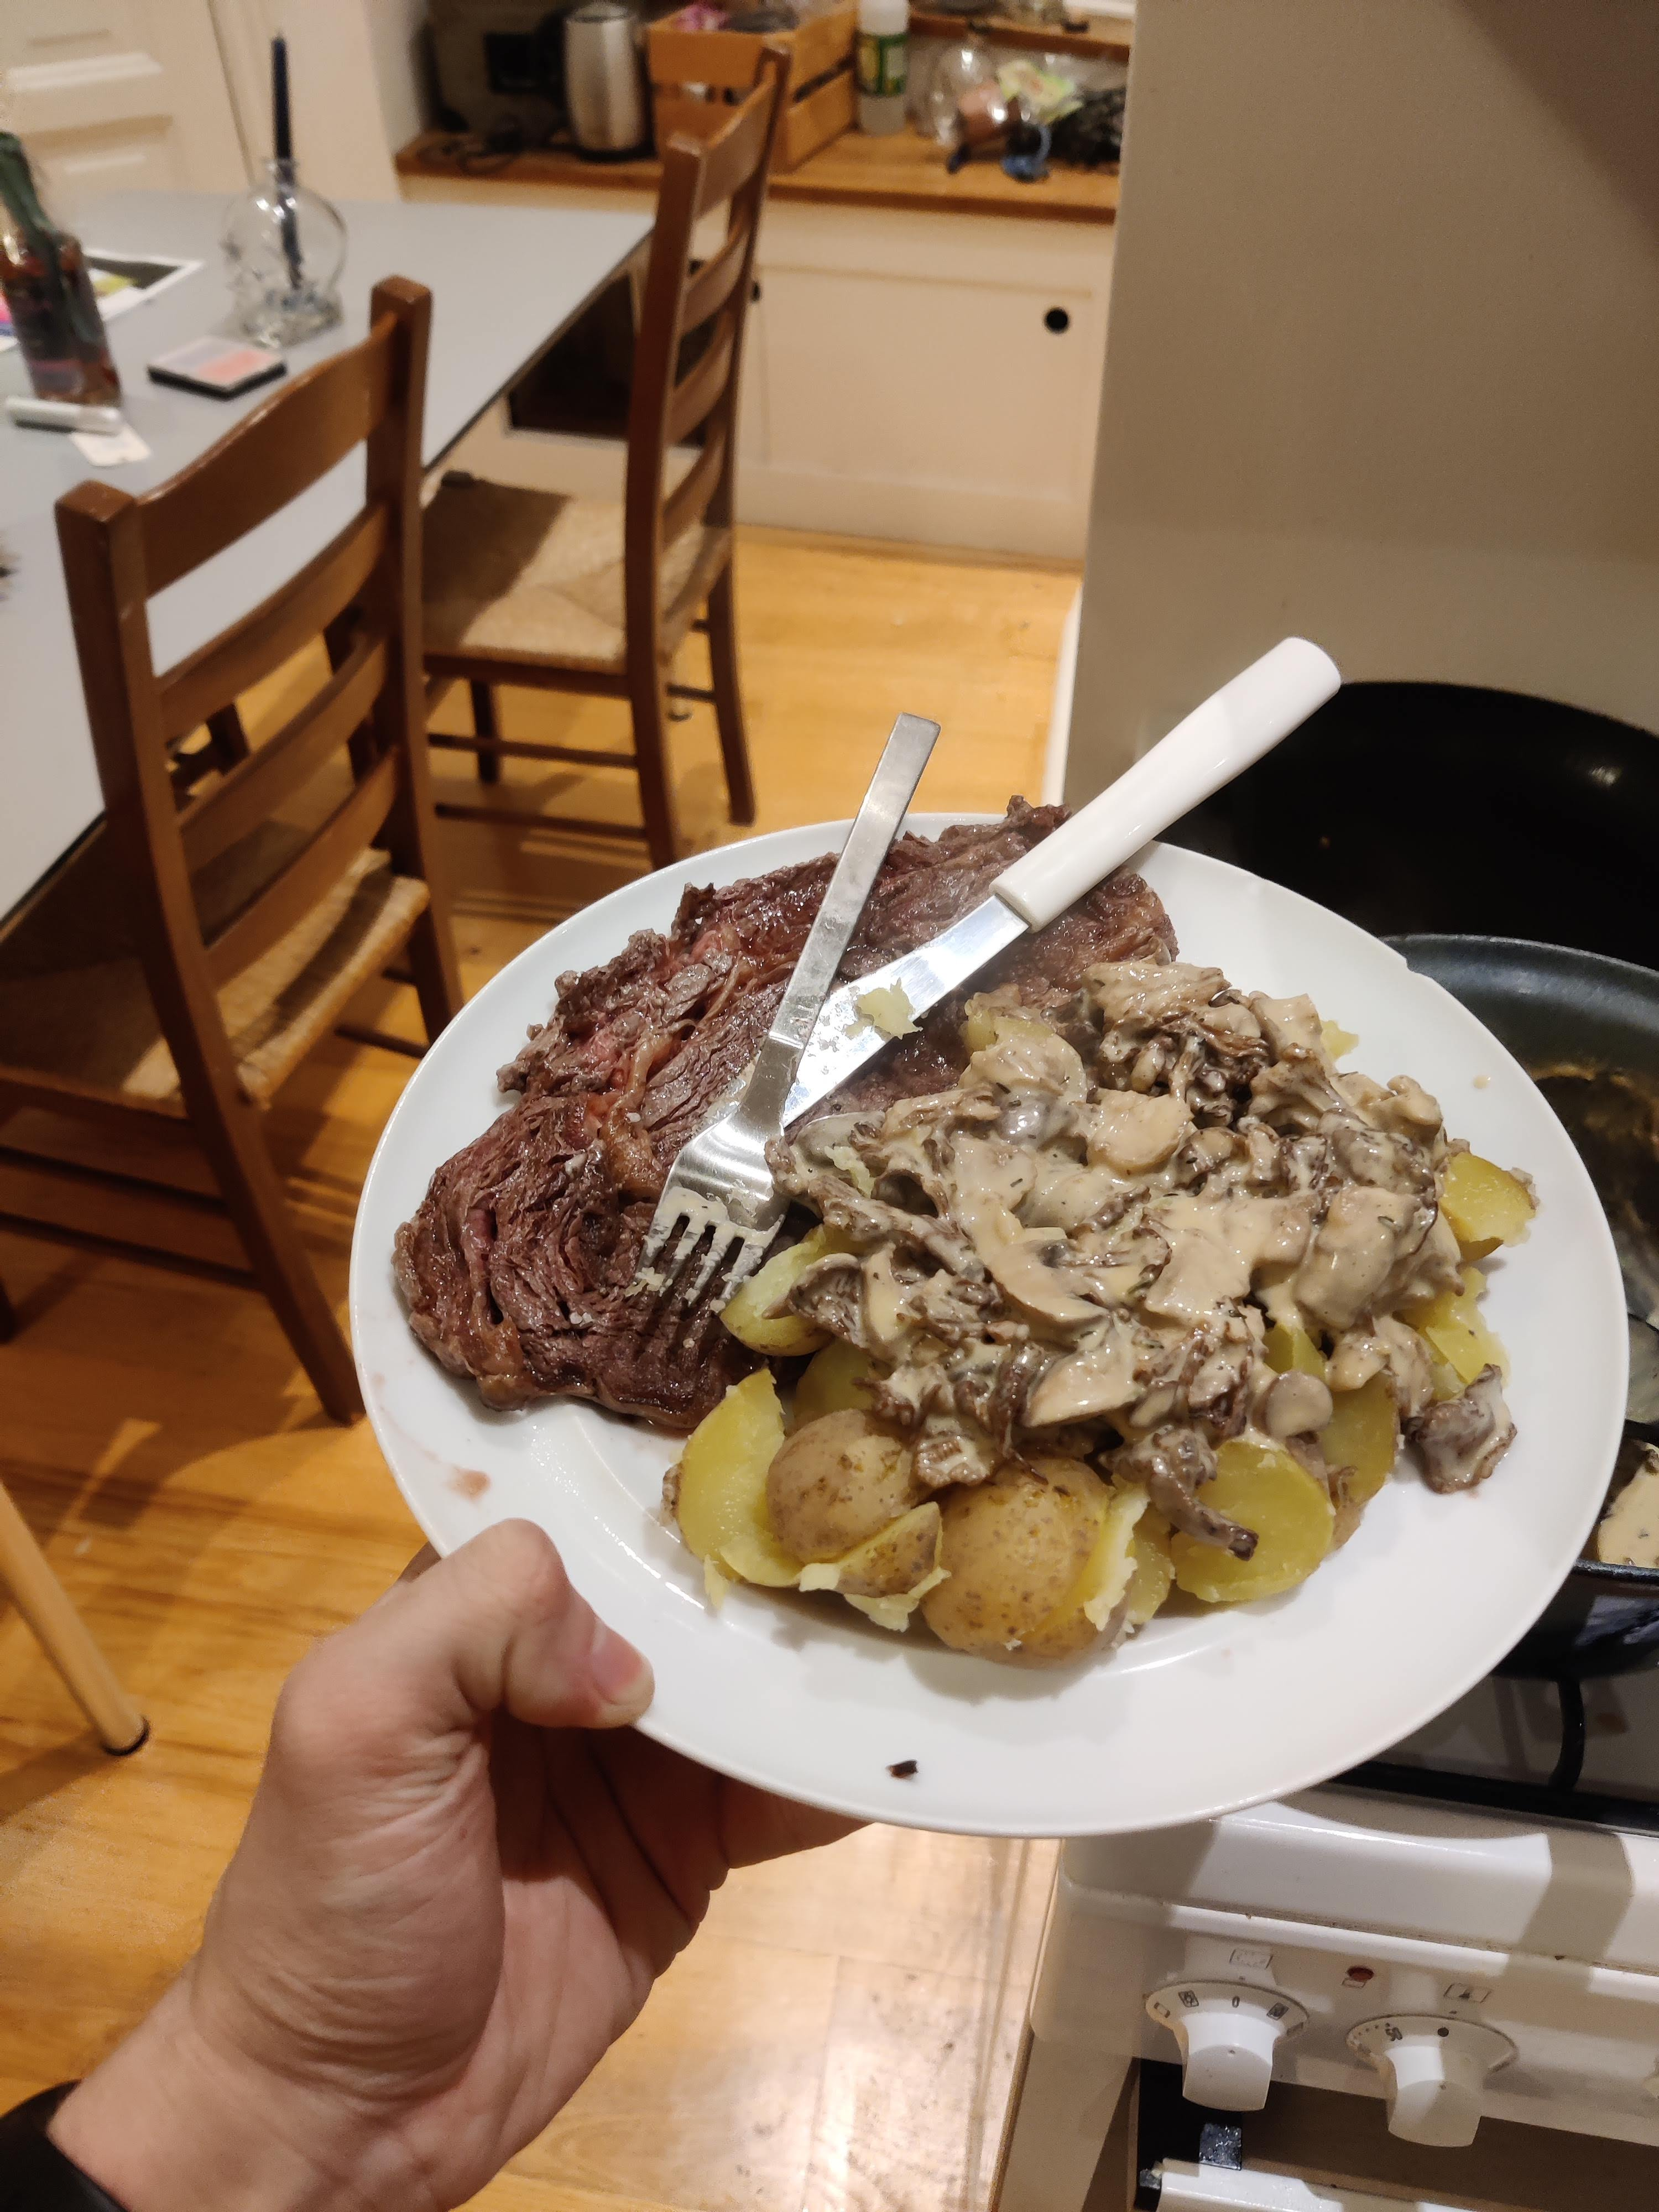
\includegraphics[width=\paperwidth,height=\paperheight]{Billeder/Tilbehør/Svampesauce.jpg}
    };
\end{tikzpicture}
\newpage \section{Tzaziki/Raita}
\begin{minipage}[t]{0.5\textwidth}
\textbf{Ingredienser:}
\begin{itemize}
    \item 1/2 agurk
    \item 1 håndfyld frisk mynte
    \item 2 fed hvidløg
    \item 200 mL græsk yoghurt (teknisk set yoghurt natural til raita)
    \item salt og pebber
    \item Eventuelt en smulle citronsaft
\end{itemize}
\end{minipage}
\begin{minipage}[t]{0.5\textwidth}
\textbf{Fremgangsmåde:}
\begin{enumerate}
    \item Riv agurken på et mandolin jern til tynde skive.
    \item Mas så meget af væsken som muligt ud af agurkeskiverne.
    \item Bland dernæst alle ingredienserne
\end{enumerate}
\end{minipage}
\newpage 
Igen mangler desværre et billede 
\begin{figure}
    \centering
    \includegraphics[width=0.5\linewidth]{Lego.jpg}
    \caption{Mig der i et shopping center i Virginia så en LEGO butik}
    
\end{figure}
\newpage \section{Hvide Asparges i brunede smør}
\begin{minipage}[t]{0.5\textwidth}
\begin{itemize}
    \item 200g hvide asparges 
    \item 50g smør
    \item Salt
\end{itemize}
\end{minipage}
\begin{minipage}[t]{0.5\textwidth}
\begin{enumerate}
    \item Smelt smøren i en kasserolle.
    \item Dernæst bag de hvide asparges i ovnen ved 200 \degree C dækkede af det brunede smør
\end{enumerate}
\end{minipage}
\newpage 
Og desværre også her 
\begin{figure}
    \centering
    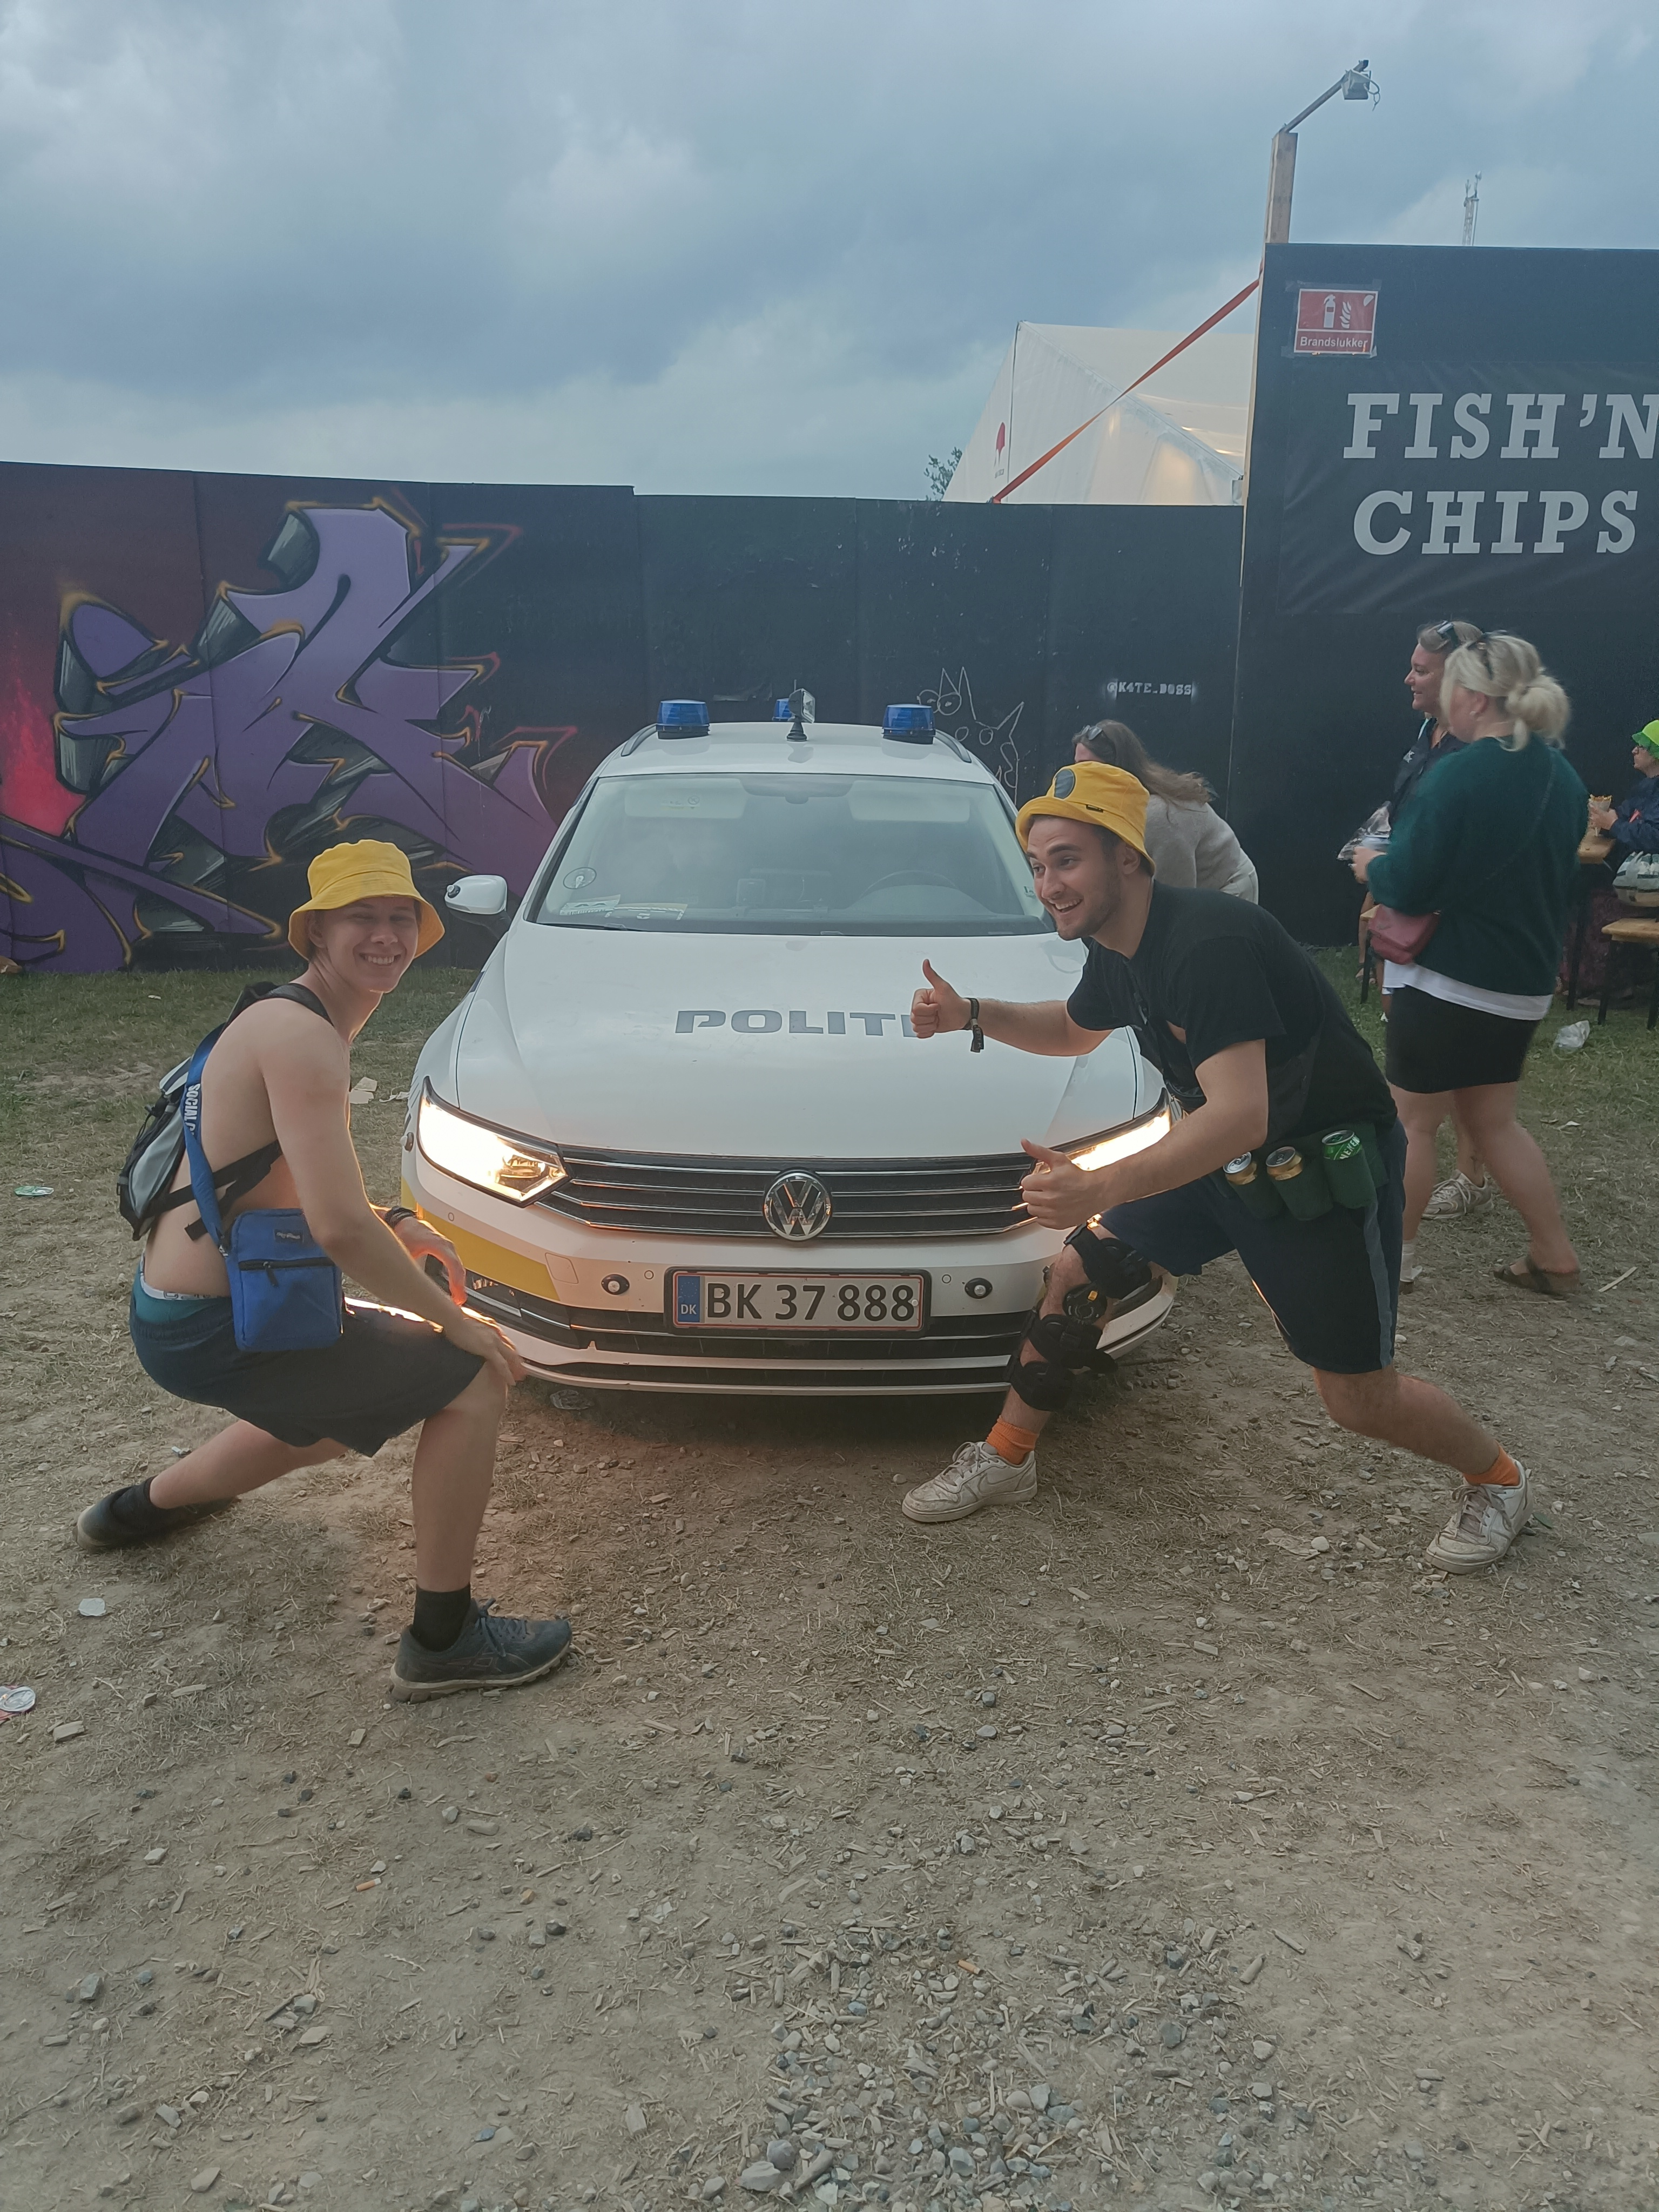
\includegraphics[width=0.5\linewidth]{Roskilde.jpg}
    \caption{Andrey og jeg foran en politi bil på Roskilde}
    
\end{figure}
\chapter{De søde sager}
\minitoc
\newpage\section{Banankage}
\begin{minipage}[t]{0.6\textwidth}
\textbf{Ingredienser:}
\begin{itemize}
  \item 150g smør
  \item 175 g sukker
  \item 1 tsk vaniljesukker
  \item 4 æg
  \item 5 banan, meget modne
  \begin{enumerate}
    \item evt 75g hakkede chokolade
    \item evt. 40g val- eller hasselnødder
  \end{enumerate}
  \item  175 g hvedemel
   \item1  tsk bagepulver
   \item 1 knivspids salt 
\\ \underline{Topping:}
 \item 100g Smeltet chokolade
\begin{enumerate}
    \item evt. 80g hakket hasselnødder
    \item evt. en smule flormeleis
\end{enumerate} 
\end{itemize}
\end{minipage}
\begin{minipage}[t]{0.4\textwidth}
\textbf{Fremgangsmåde}
\begin{enumerate}
   \item  Start med at smelte smøren og pisk sammen med sukker og vaniljesukker. 
   \item  Mos bananerne og tilsæt.
   \item  Dernæst tilsæt æggene en af gangen og chokolade og sukker.
   \item  Rør bagepulver, mel og salten i.
   \item  Hæld dejen i den ønskede form (f.eks. en springfrom med smurte sidder, ellers kan en bradepande også gå an), og smid i ovnen på 175 \degree C i 45 minutter
   \item  Hæld den smeltet chokolade på den varme kage og drys de hakkede nødder på 
\end{enumerate}
\end{minipage}
Hvis man ønsker at lave banankage men ikke har nogle overmodne bananer, kan man få den samme effekt ved at smide dem i fryseren, dette nedbyrder cellevæggen.
\newpage
\begin{tikzpicture}[remember picture,overlay,inner sep=0pt,outer sep=0pt]
    \node[anchor=south east] at (current page.south east) { 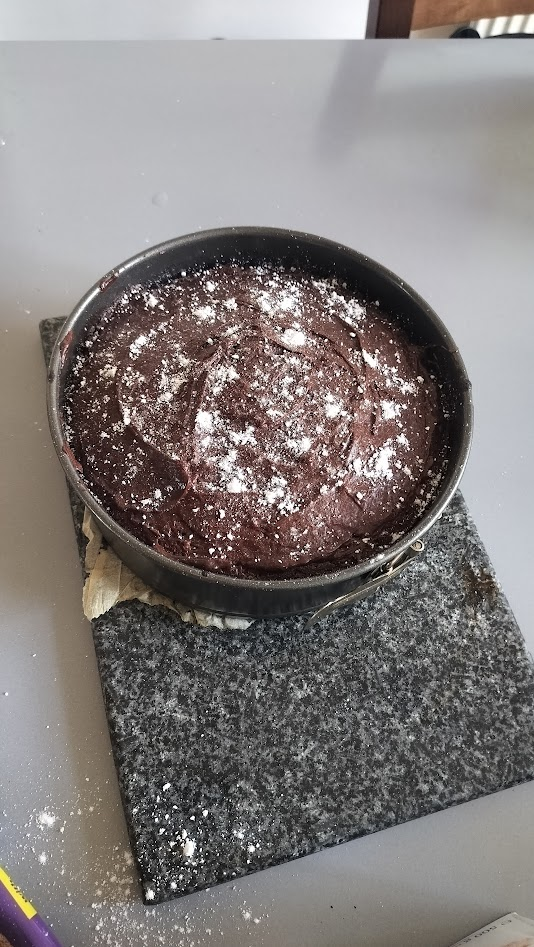
\includegraphics[width=\paperwidth,height=\paperheight]{Billeder/Dessert/banankage2.jpg} };
\end{tikzpicture}
%\newpage \section{Browine}
%begin{minipage}[t]{0.5\textwidth}
%\end{minipage}
%\begin{minipage}[t]{0.5\textwidth}
%\end{minipage}
\newpage \section{Gode Råd}
\begin{minipage}[t]{0.5\textwidth}
\textbf{Ingredienser:}
\begin{itemize}
    \item 3 æg
    \item 100 g sukker
    \item 250 g hvedemel
    \item 1.5 tsk kardemomme 
    \item 125 g smeltet margerine
    \item 1/2 dL mælk
\end{itemize}
\end{minipage}
\begin{minipage}[t]{0.5\textwidth}
\textbf{Fremgangsmåde:}
\begin{enumerate}
    \item Pisk æg 
    \item 
    \item Bag i vaffeljern til gyldenbrun
\end{enumerate}
\end{minipage}
\begin{figure}
    \centering
    \includegraphics[width=0.5\linewidth]{Billeder//Dessert/Gode råd.jpg}
    \caption{Farmors opskift på gode råd}
\end{figure}
\newpage \section{Ris a la Mande}
\begin{minipage}[t]{0.5\textwidth}
\textbf{Ingredienser:}
\begin{itemize}
    \item 1L sød mælk
    \item 75 g sukker
    \item 1 stk vaniljestang, flækket (skåret over langs midten)
    \item 180 g grødris
    \item 100 g mandler, hakkede
    \item 1 knivspids salt
    \item 4 dL piskefløde
\end{itemize}
\end{minipage}
\begin{minipage}[t]{0.5\textwidth}
\begin{enumerate}
    \item Bring sødemælk i kog under opsyn (rør i den en gang imellem).
    \item Skru ned for varmen når sødmælken begynder at dampe, og ad stå under låg i 2 minutter.
    \item Vend den flækket vaniljestang i sukker således vanilje kornene inden i ikke klumper, og smid det hele (inklusiv den hele stang, i mælken. 
\end{enumerate}
\end{minipage}
\newpage 
\newpage \section{Marengs}
\begin{minipage}[t]{0.5\textwidth}
\textbf{Ingredienser:}
\begin{itemize}
    \item 140 g æggehvider
    \item \~ 300 g floremelis
\end{itemize}
\end{minipage}
\begin{minipage}[t]{0.5\textwidth}
\textbf{Fremgangsmåde:}
\begin{enumerate}
    \item Forvarm ovn til 80 \degree C
    \item Pisk æggeviden til de ikke længere er gennemsigtige
    \item Tilføj dernæst flormelisen lidt efter lidt
    \begin{itemize}
        \item At tilføje flormelis til æggehviden minder meget om når man laver glasur, tilsæt de lidt efter lidt til det til sidst er "svært" at opløse mere flormelis i
    \end{itemize}
    \item Pisk mere end man umiddelbart skulle tro, det skal blive meget luftigt
    \item Put ned i pose, til at trykke ud som "kys". Eller hæld i springform til brug til kage
    \item Bag i ovnen ved 80 \degree C i \~ \space 1 time
    \item Til sidst kan der eventuelt skrues op for varmen, men dette giver "pludselig" udvidelse af marengsne, men sikre de bliver færdige.
\end{enumerate}
\end{minipage}
OBS. Prøv at lave dem så tynde/luftige som mulige da de ellers kan blive klistretret indeni, og vil dermed forårsage at de bliver lidt gyldne/ en smule brændte 
\newpage \begin{tikzpicture}[remember picture,overlay,inner sep=0pt,outer sep=0pt]
    \node[anchor=south east] at (current page.south east) {
        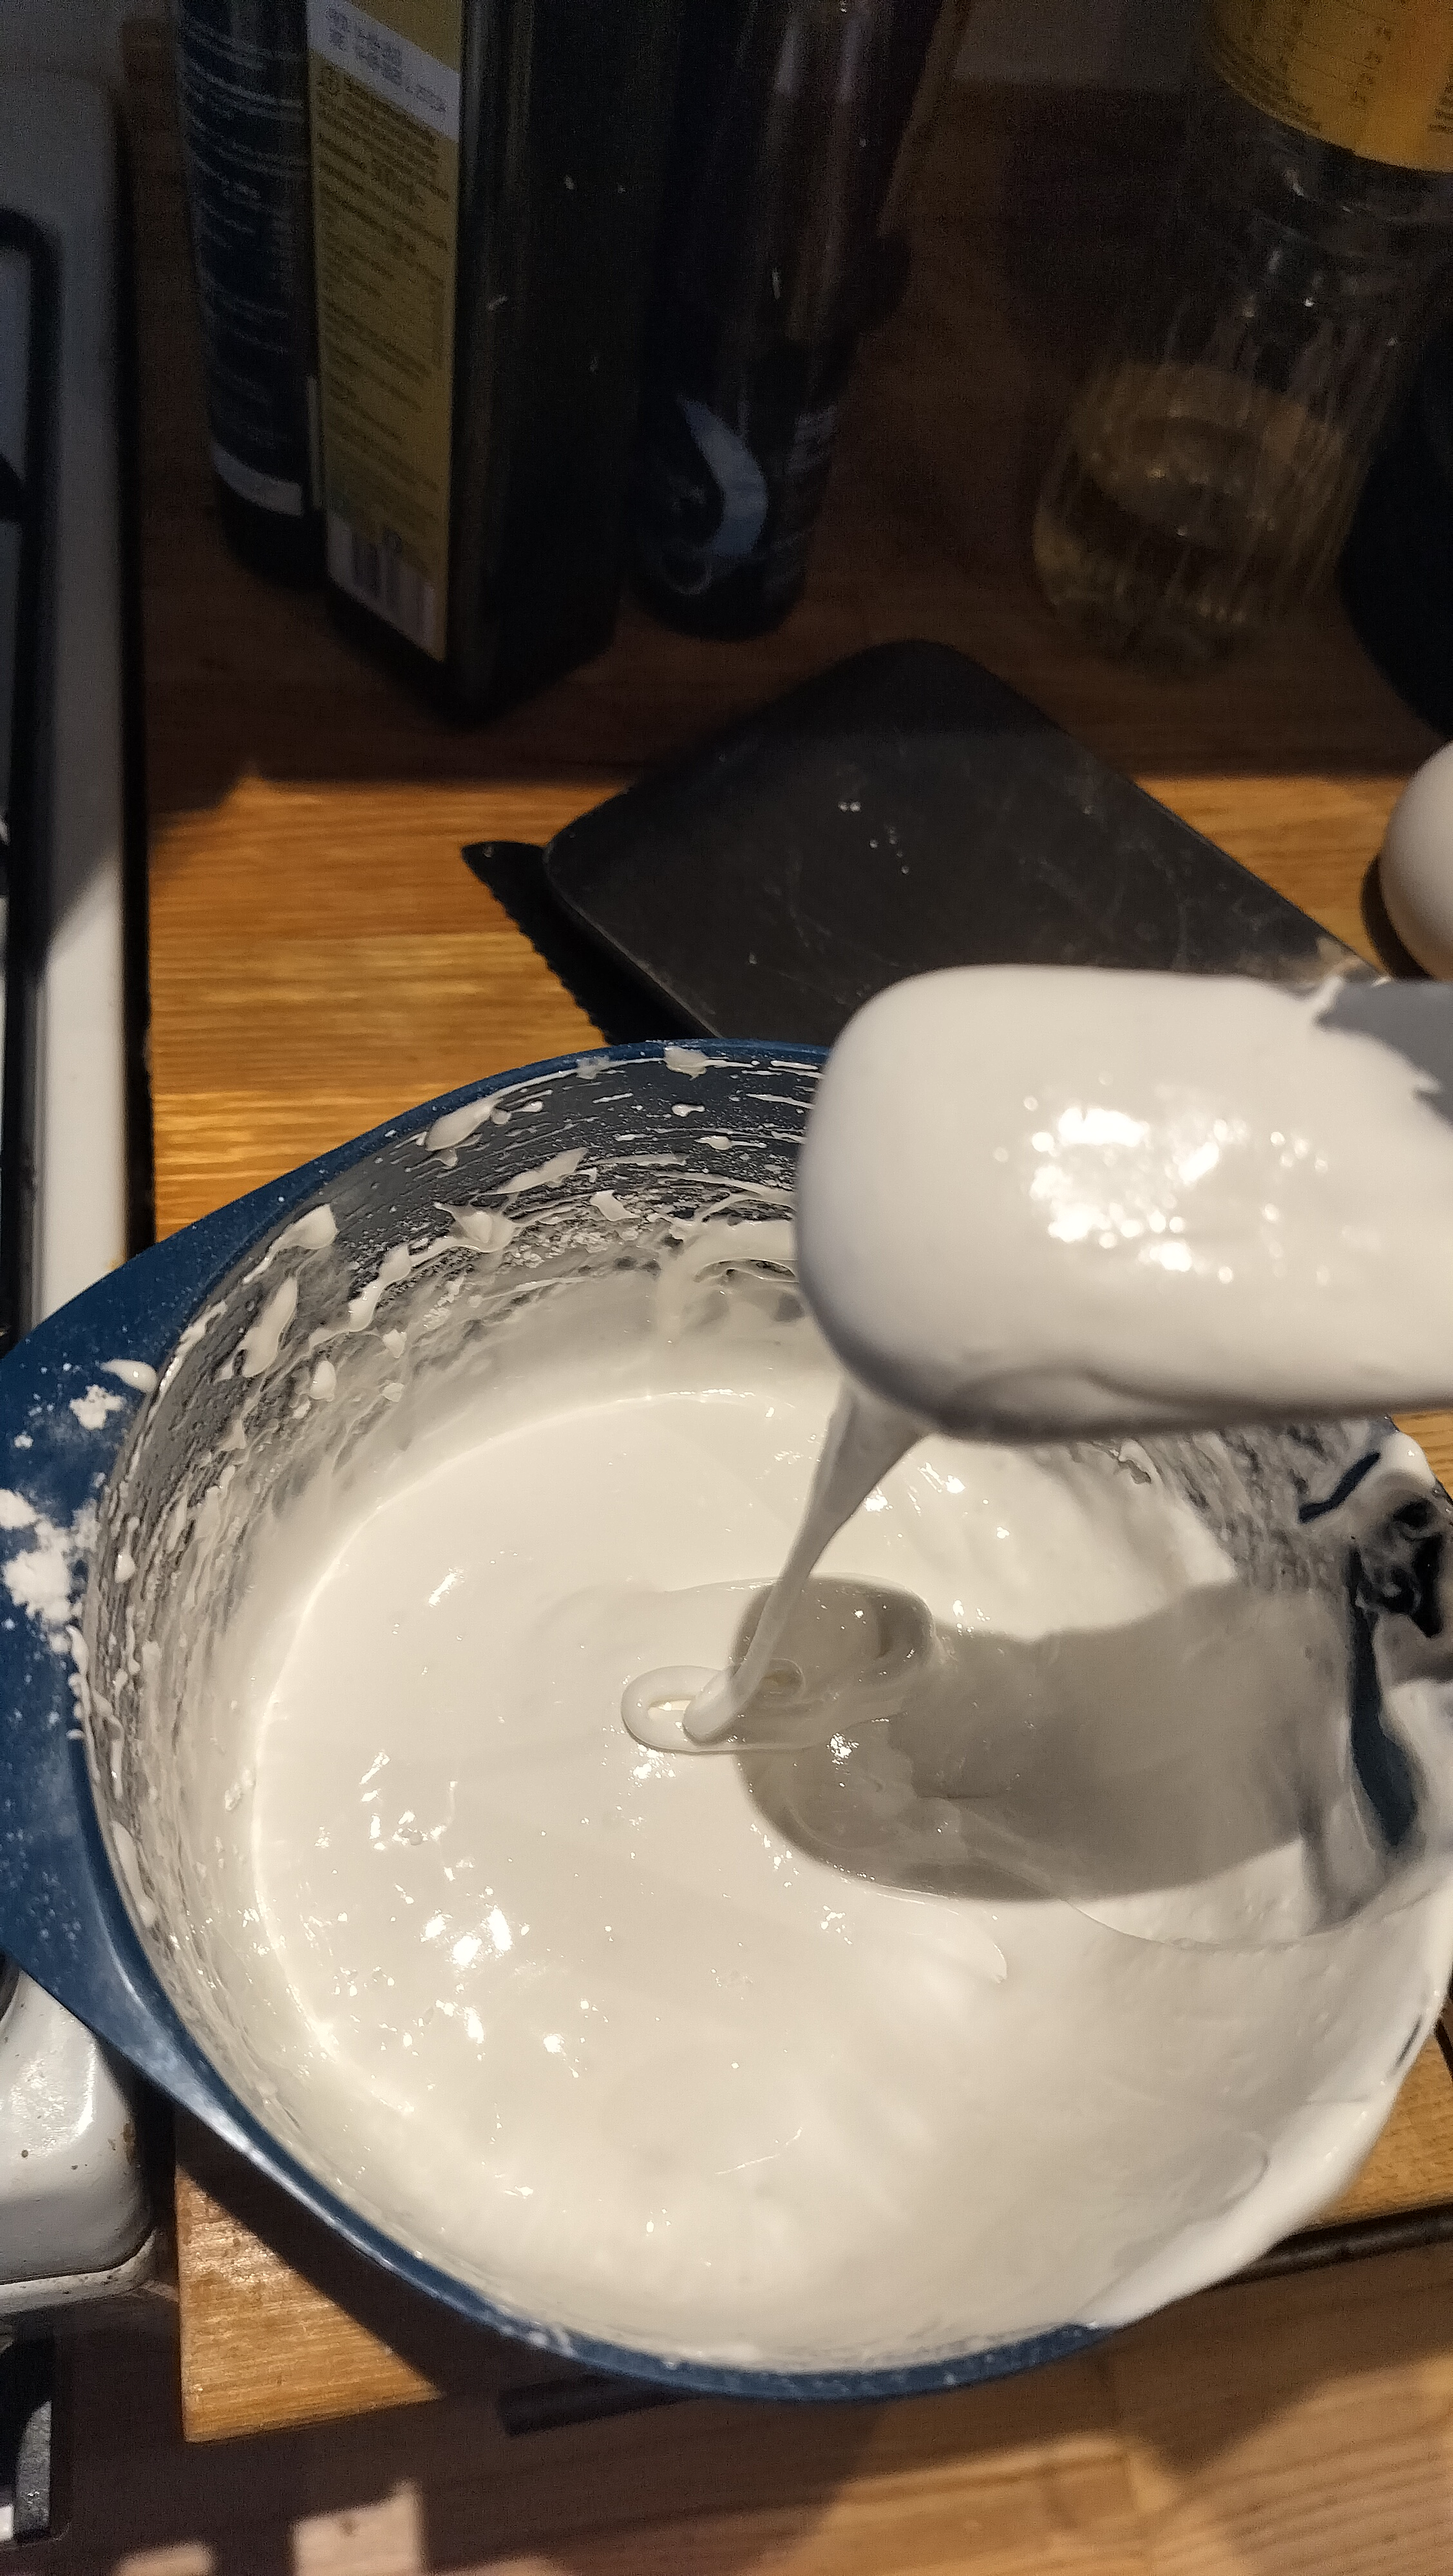
\includegraphics[width=\paperwidth,height=\paperheight]{Billeder/Dessert/Marengs_Flydende.jpg}
    };
\end{tikzpicture}
\chapter{Brød}
\minitoc
Synes især at jeg har haft stor succes i forhold til bagning af brød, har som udgangspunkt ikke talt det med som en ny af de månedlige opskrifter. Har desværre ikke været så god til at huske at tage billeder af brødet så lige nu kommer det bare til at være arbitære billeder.
\newpage \section{Brioche}
\begin{minipage}[t]{0.5\textwidth}
\textbf{Ingredienser:}
\begin{itemize}
    \item 3 dl mælk
    \item 25 g gær
    \item 2 æg
    \item 125 g smør, skåret i tern, stuetempereret
    \item 2 spsk sukker
    \item 1.50 tsk salt
    \item 1 knivspids stødt kardemomme
    \item 550 g hvedemel
\end{itemize}
Pensling:
\begin{itemize}
    \item 1 æg
    \item Evt. sesamfrø
    \item Evt. græskarkerne
\end{itemize}
\end{minipage}
\begin{minipage}[t]{0.5\textwidth}
\textbf{Fremgangsmåde:}
\begin{enumerate}
    \item Varm mælken til lunken, og rør gøren ud i.
    \item Tilsæt æg, smør, sukker, salt, kardemomme og 250g af hvedemellen.
    \item Rør dejen sammen til ensartet konsistens, tilsæt dejen lidt efter lidt.
    \item Lad dejen hæve i 2 timer ved stuetemperatur.
    \item Form dejen til boller (cirka 10), og lad dem stå til hævning i en time.
    \item Pensel med æg og tilsæt ønskede krydderie, og bag i forvarmet ovn på 175 \degree C varmluft i omtrent 20 minutter
\end{enumerate}
\end{minipage}
\newpage Her kunne der være et billede af nogle briocheboller, men i stedet for er der et billede af Artemis
\begin{figure}
    \centering
    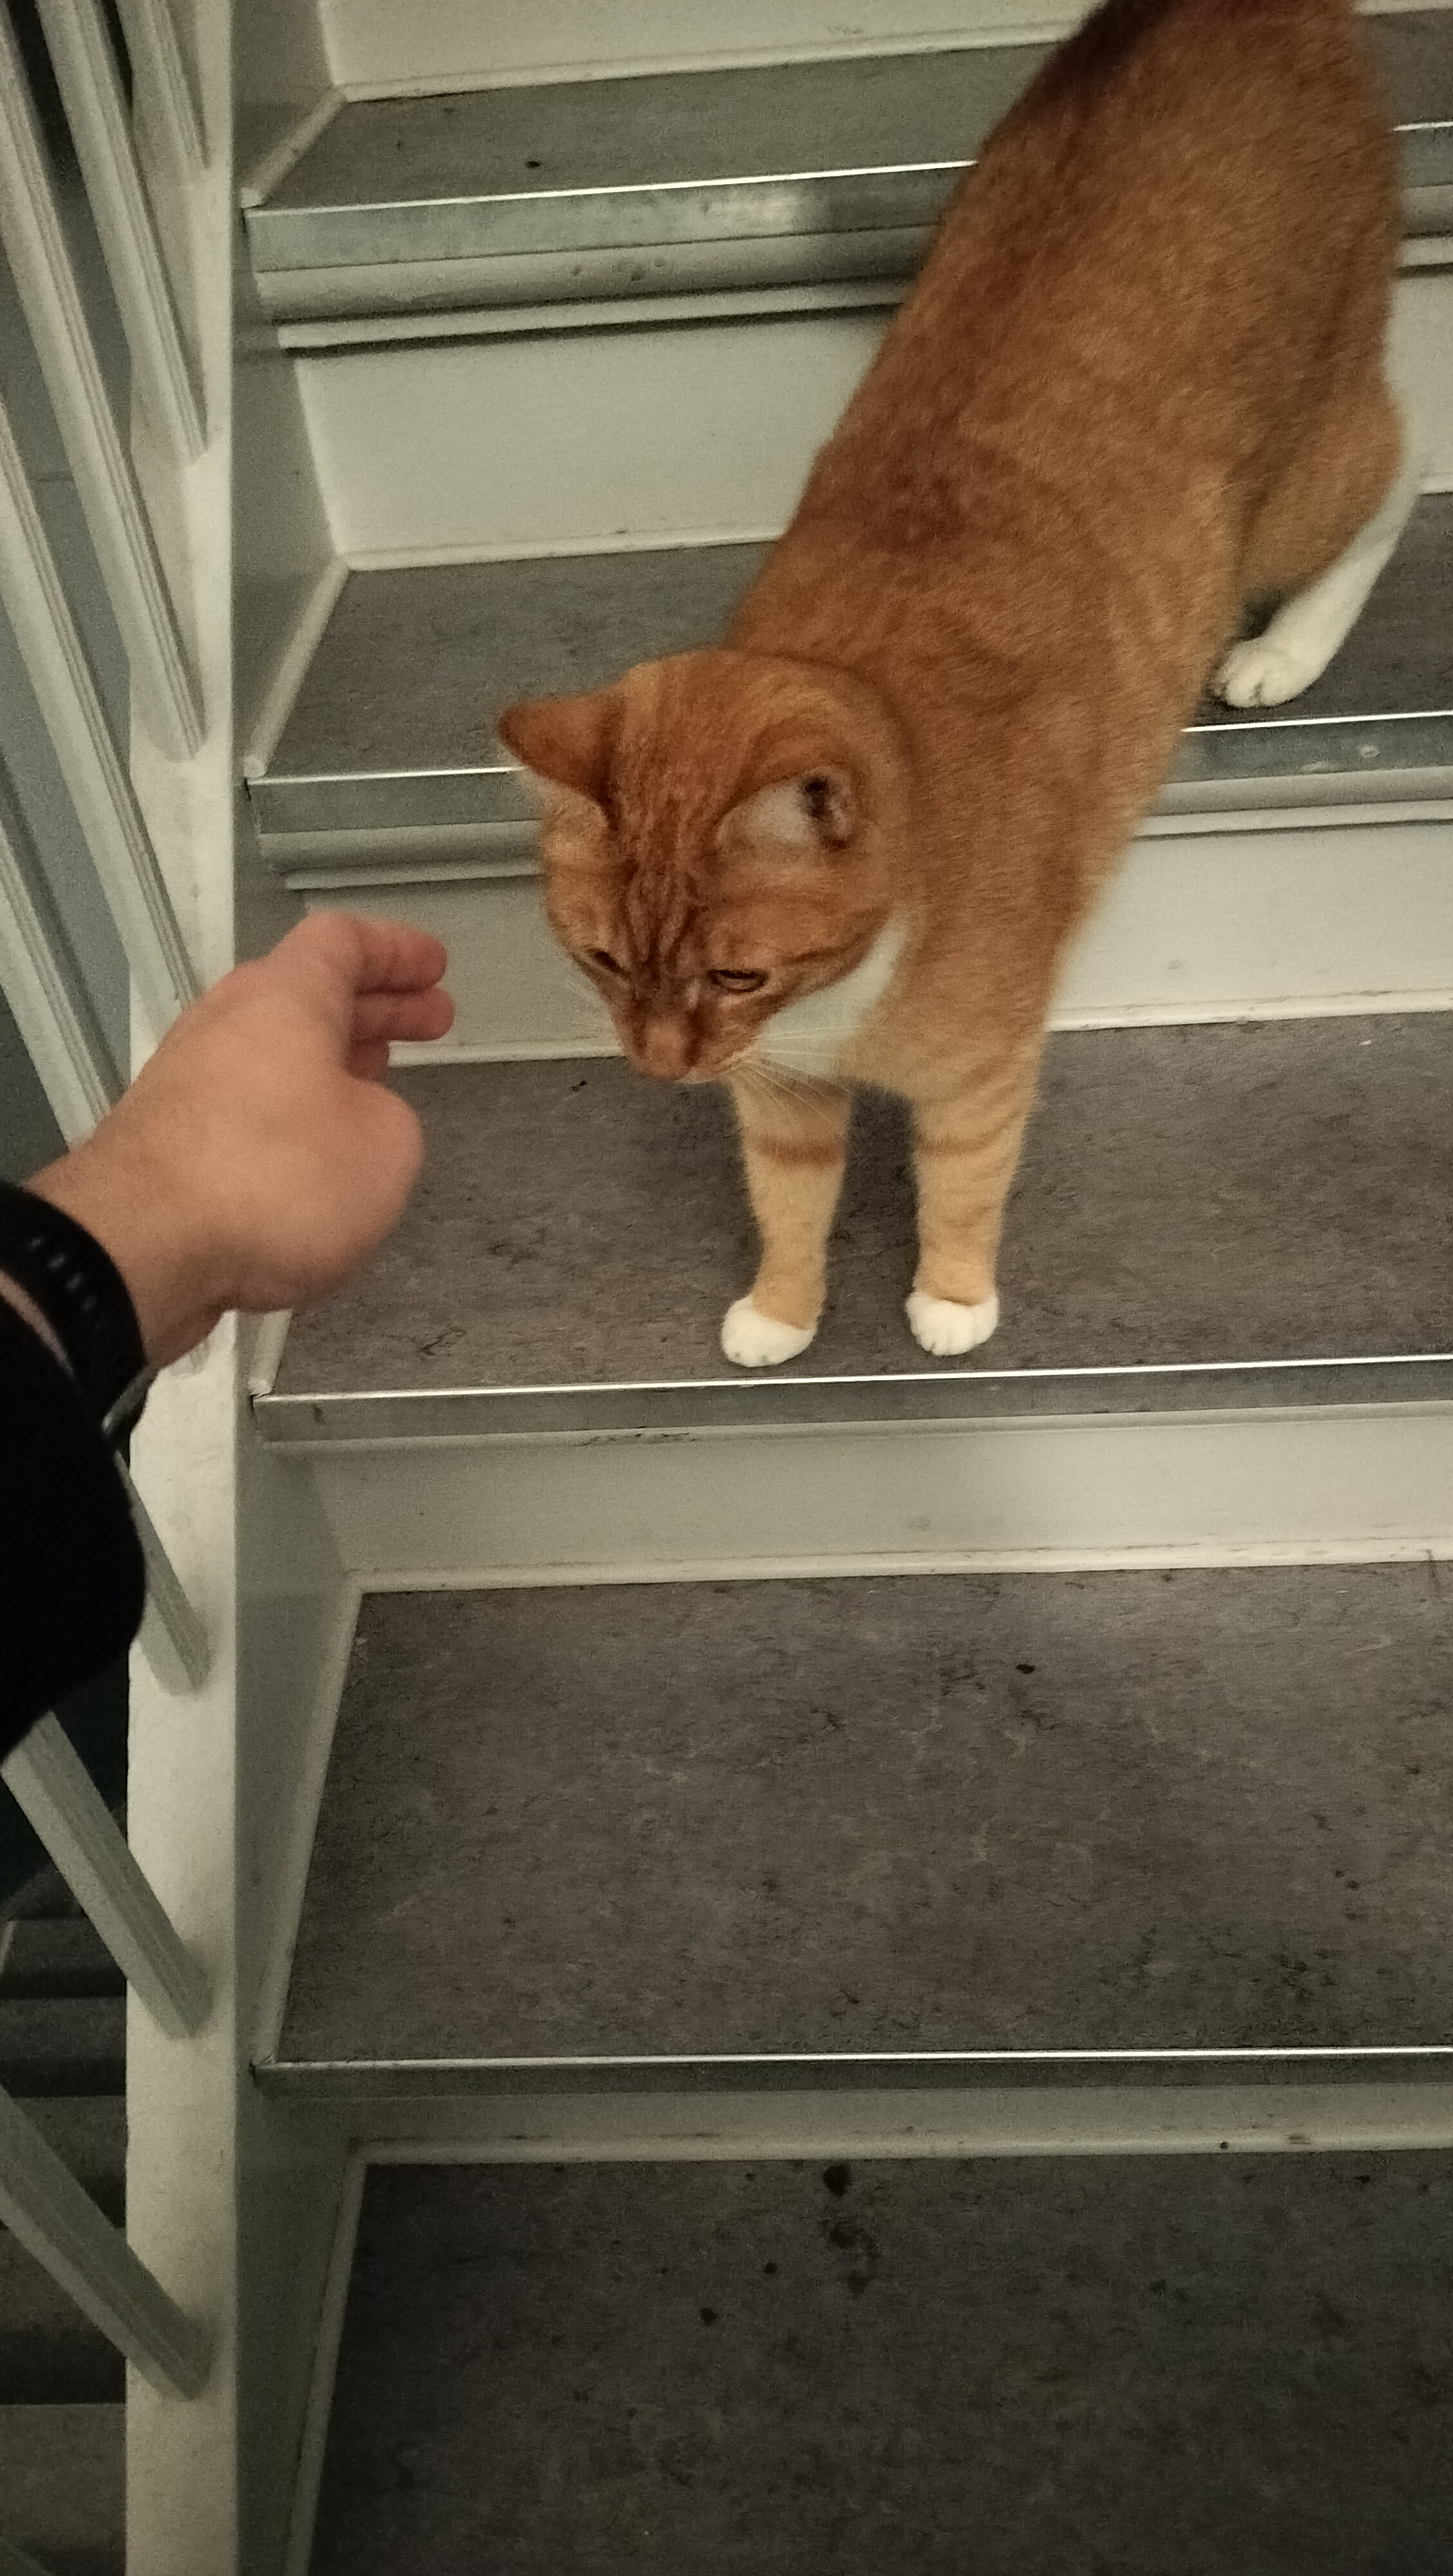
\includegraphics[width=0.5\linewidth]{IMG20231108195607.jpg}
    \caption{Artemis}
\end{figure}
\newpage \section{Ciabatta}
\begin{minipage}[t]{0.5\textwidth}
\textbf{Ingredienser:}
\begin{itemize}
    \item 7 dL lunkent vand (stuetemperatur)
    \item 10 g gær
    \item 2 tsk sukker
    \item 2 tsk salt
    \item 800 manitoba hvedemel
\end{itemize}
Pensling
\begin{itemize}
    \item 2 spsk olivenolie
    \item Evt. Timian
    \item Flagelsalt eller groftsalt
\end{itemize}
\end{minipage}
\begin{minipage}[t]{0.5\textwidth}
\textbf{Fremgangsmåde:}
\begin{enumerate}
    \item Hæld vandet i en skål, og rør sukker og gær ud.
    \item Tilsæt melem og salten til vandet.
    \item Rør dejen til en ensartet masse, dæk til med viskestykke og lad hæve i 5 timer.
    \item Hæld dejen ud på et mel dækket bord, og fold dejen gentagende gange.
    \item Del dejen i 2 stykker, pensel med olivenolie, og lig på en bageplade.
    \item Bag i en forvarmet ovn på 275 \degree C varmluft.
\end{enumerate}
\end{minipage}
\newpage Her skulle der også været et billede, så der kommet et billede af Devils Starways
\begin{figure}
    \centering
    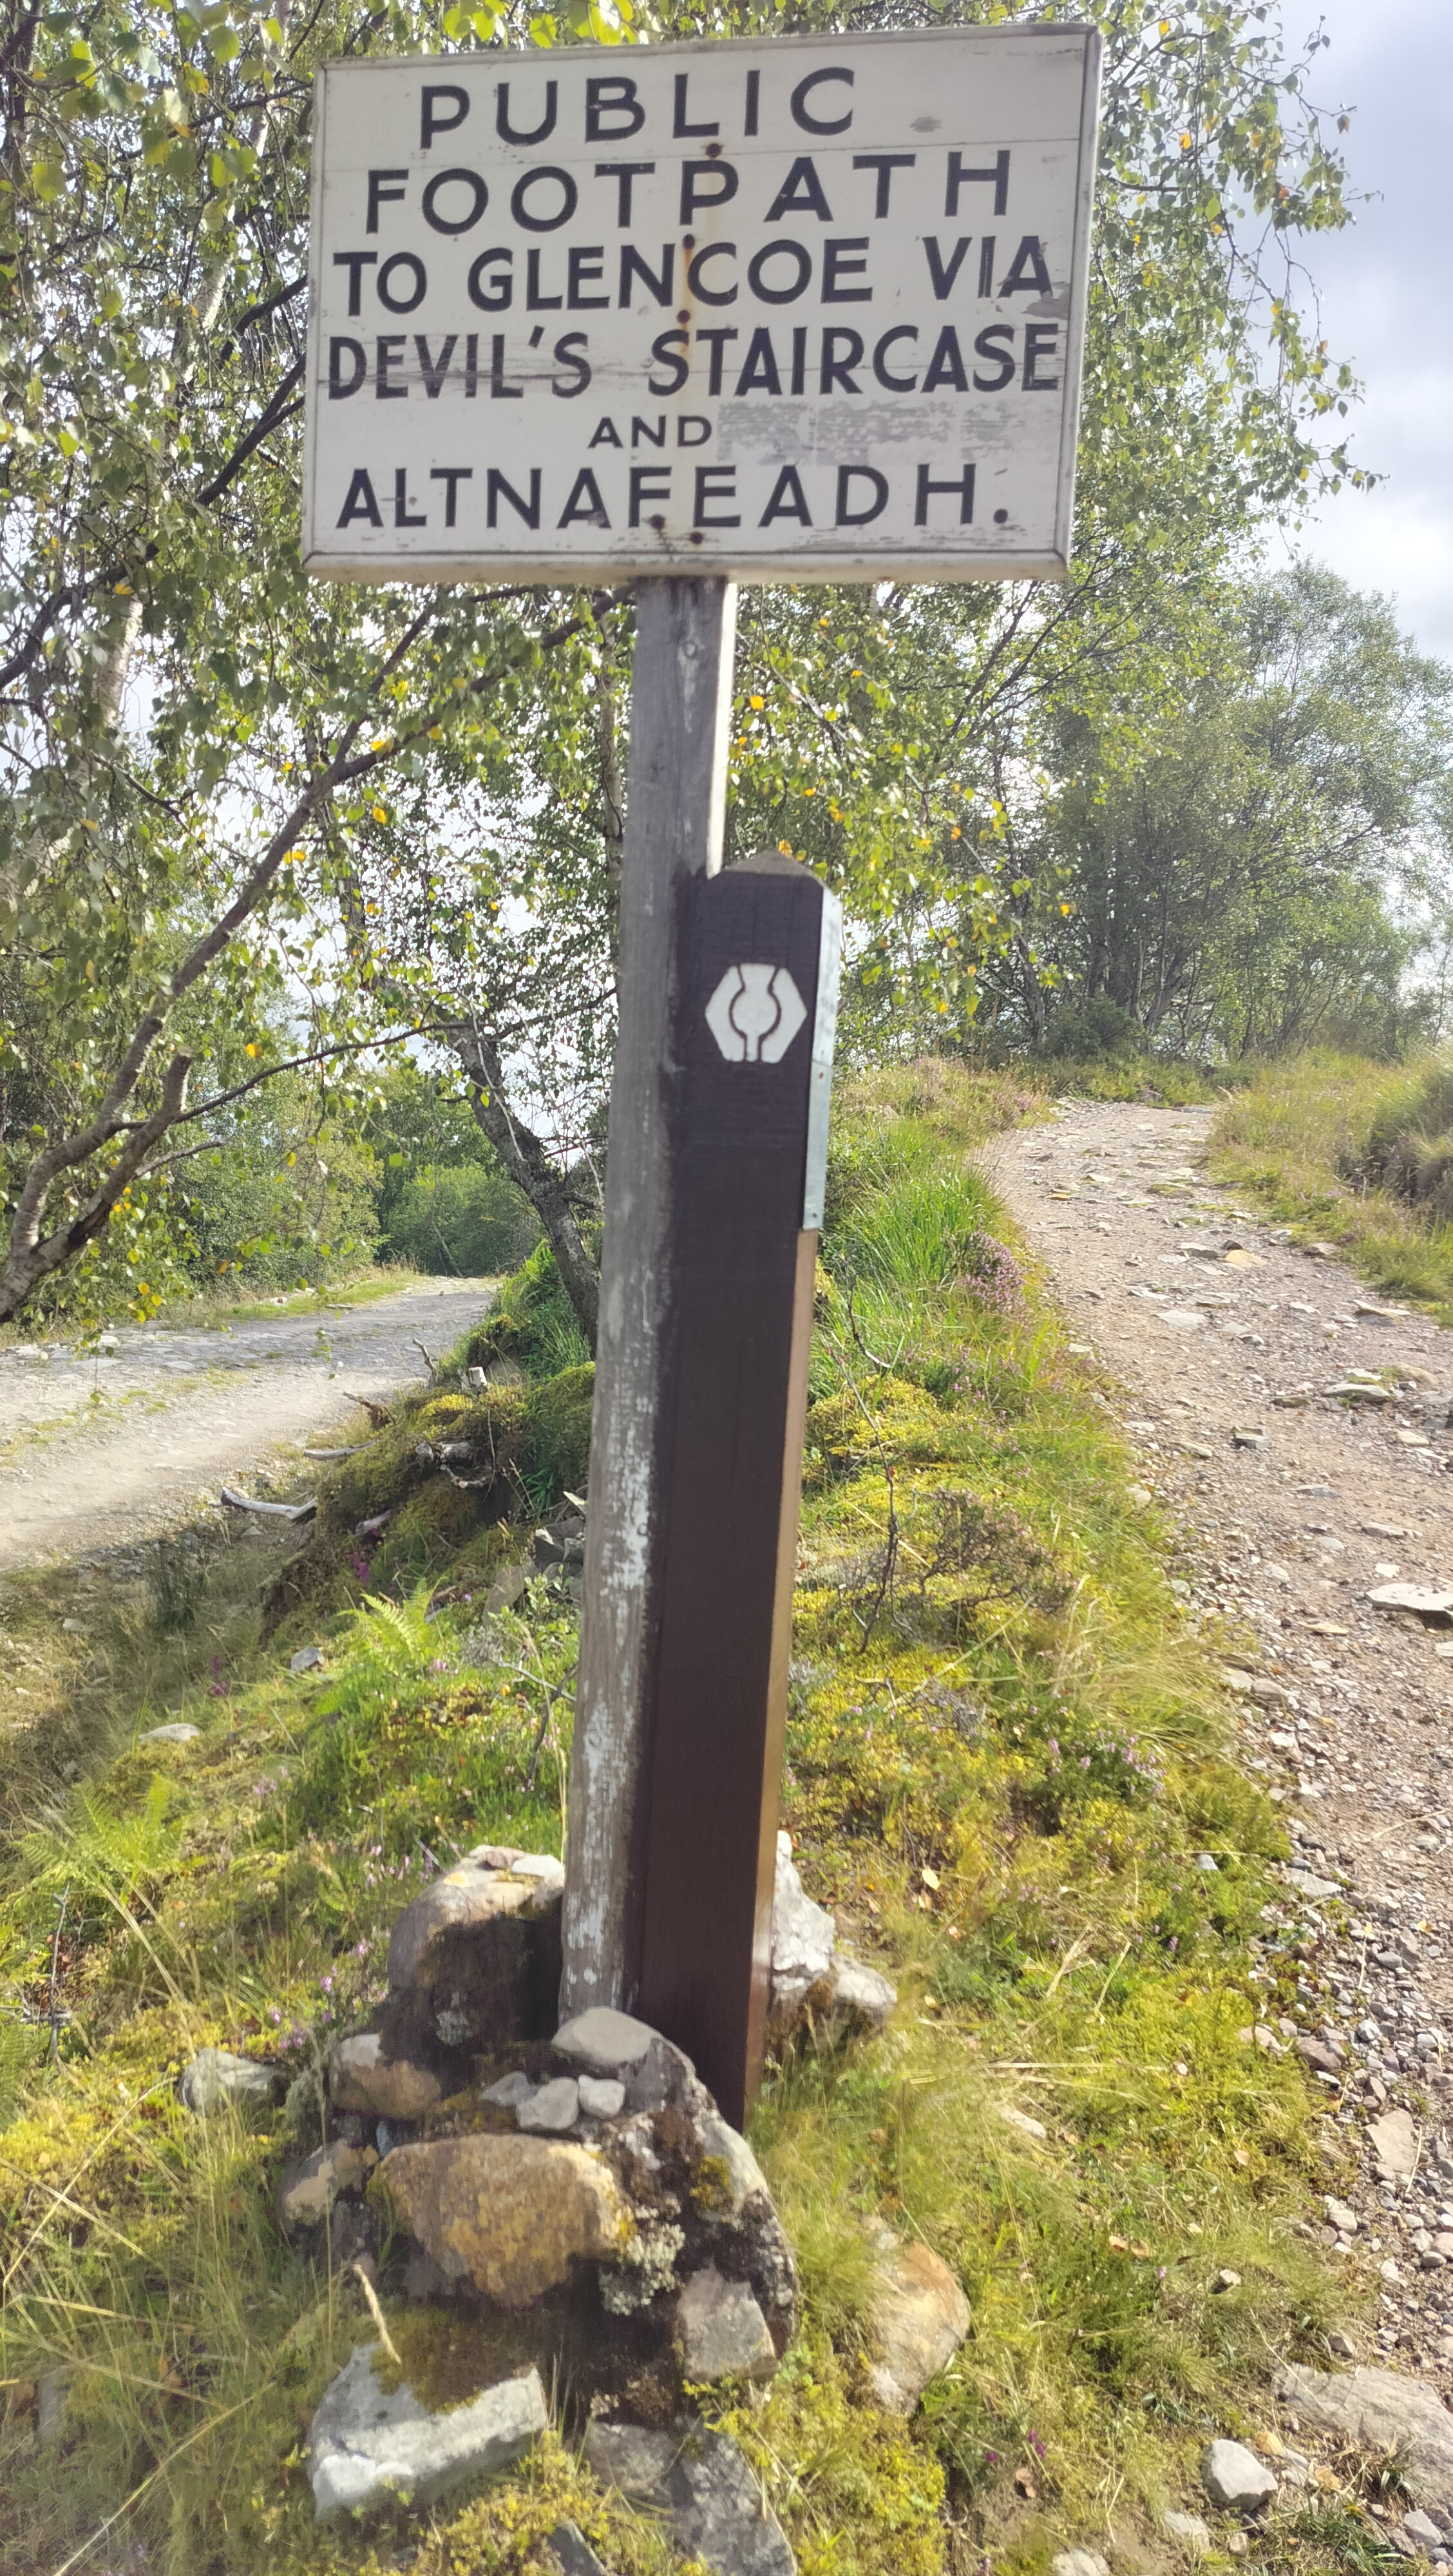
\includegraphics[width=0.5\linewidth]{Devils_stairway.jpg}
    \caption{Devils stairway}
\end{figure}
\newpage \section{Focaccia}
\begin{minipage}[t]{0.5\textwidth}
\textbf{Ingredienser:}
\begin{itemize}
    \item 4 dL vand
    \item 20 g gær
    \item 3 spsk olivenolie
    \item 1 tsk salt
    \item 100 g grahamsmel
    \item 400 g hvedemel
\end{itemize}
Topping:
\begin{itemize}
    \item 1 tsk flagesalt (eller groft salt)
    \item 4 fed hvidløg, presset
    \item Rosmarin (eventuellet frisk)
    \item Evt. 100 g oliven, skiveskåret
    
\end{itemize}
\end{minipage}
\begin{minipage}[t]{0.5\textwidth}
\textbf{Fremgangsmåde:}
\begin{enumerate}
    \item Rør gæren ud i en skål med vand.
    \item Tilsæt olien, salten og grahamsmellen og rør rundt.
    \item Tilsæt hvedemellen lidt efter lidt, og ælt til dejen er klistret og blød.
    \item Dæk dejen til og lad den hæve i 1 time.
    \item Lig dejen ud på en bradepande, og lad den hæve en halv time yderligere.
    \item Tryk fordybninger i dejen, og pensel med olivenolie og drys de ønskede toppings.
    \item Bag i en forvarmet ovn ved 180 \degree C i 20 minutter
\end{enumerate}
\end{minipage}
\\ Når man lader dejen hæve på en bradepande er det vigtigt det ikke er for lang tid, en længerevarig hævning får brødet til at "miste" pusten, dette giver en mindre hævning under bagning og i sidste ende et mindre luftigt brød. 
Foaccaia er et relativ hurtigt brød at bage med en vente tid på omtrent 1 time og 50 minutter med 10-15 minutters arbejds tid. En samlet tid på \underline{2 timer og 5 minutter}
\newpage Her skulle der også have været et billedet, istedet for kommer der et billede af mit kostume til min 23 års fødsesldag 
\begin{figure}
    \centering
    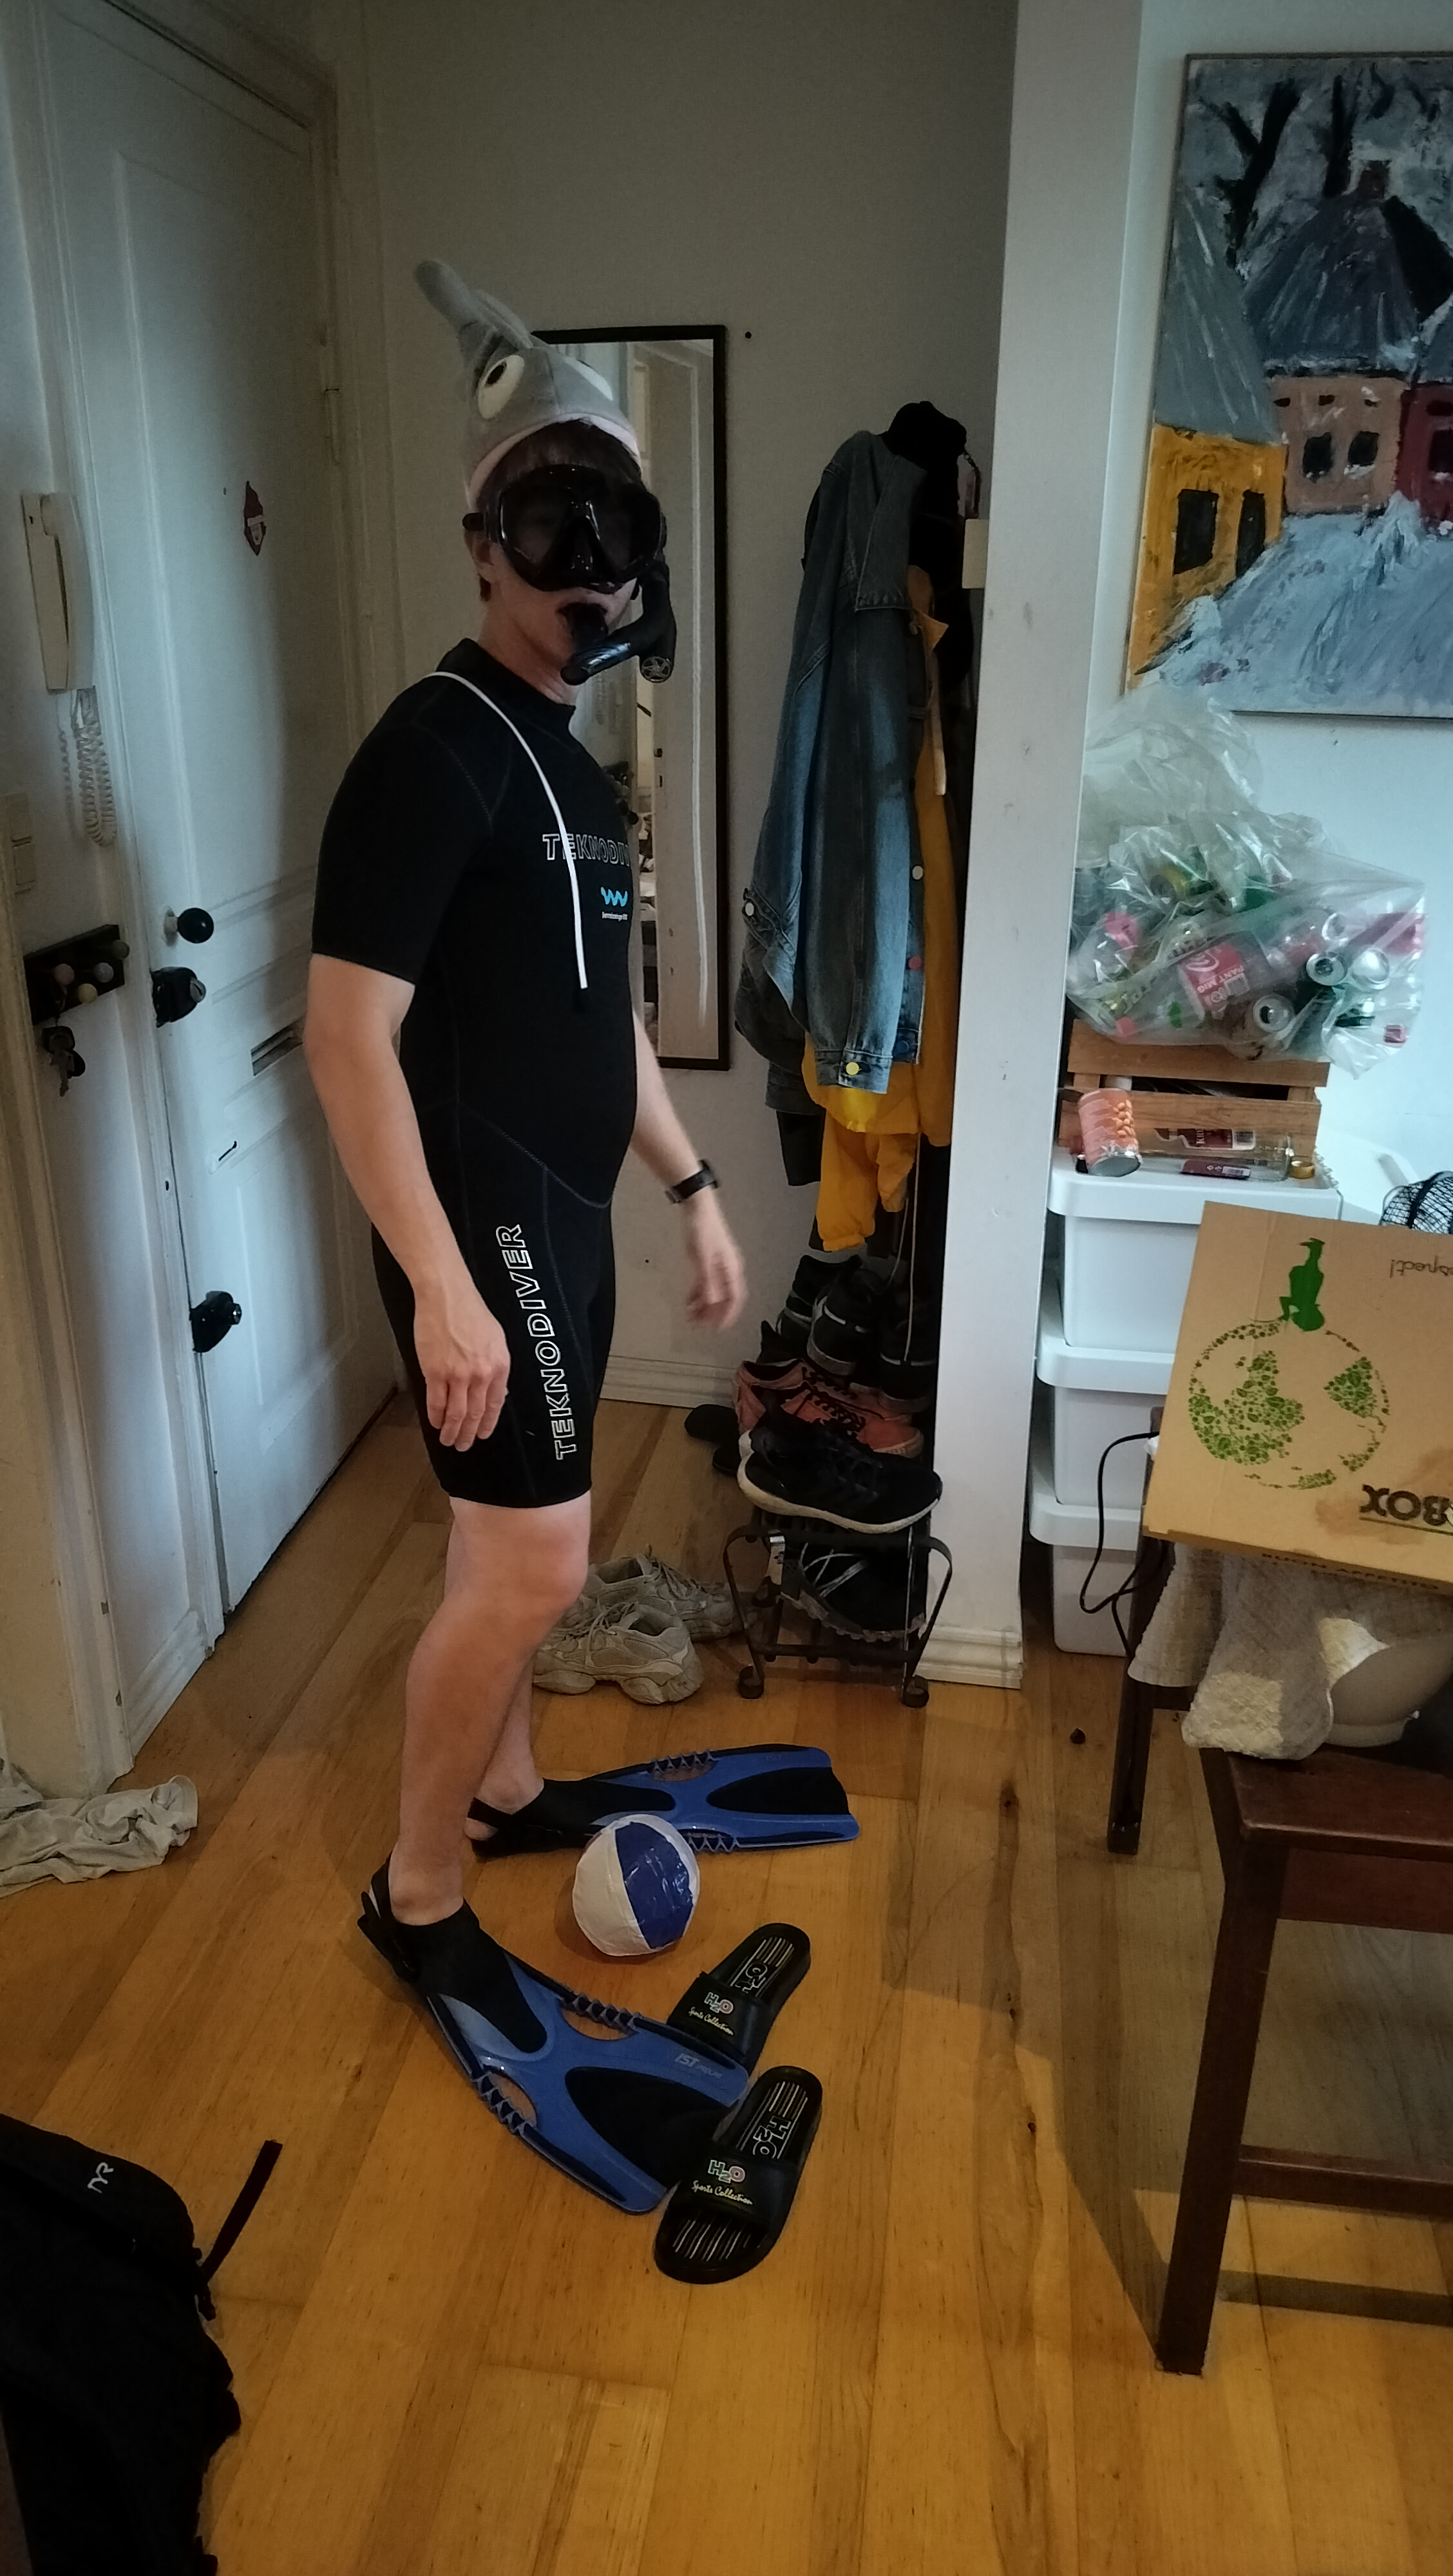
\includegraphics[width=0.5\linewidth]{Dykke.jpg}
    \caption{Dykker der brutalt bliver spist af en haj}
    
\end{figure}
\newpage \section{Naan}
\begin{minipage}[t]{0.5\textwidth}
\textbf{Ingredienser:}
\begin{itemize}
    \item 1 dl stuetempereret vand
    \item 25 g gær
    \item 1 dl mælk
    \item 1 æg, sammenpisket
    \item 1 dl græsk yoghurt 10 %
    \item 3 spsk olivenolie
    \item1 tsk salt
    \item1 tsk sukker
    \item450 g hvedemel
\end{itemize}
    Pensling og smag
\begin{itemize}
    \item 50 g smør, smeltet
    \item Fiske koriander, finthakket
    \item 2 fed hvidløg, pressede
    \begin{enumerate}
        \item  evt 1 spsk nigella frø. \\
        Nigella frø kan fås i inco og ligende, men tilføje ikke det store i forhold til smagen
    \end{enumerate}
\end{itemize}
\end{minipage}
\begin{minipage}[t]{0.5\textwidth}
\begin{enumerate}
    \item Kom vand i en skål og rør gær ud i væsken. Tilsæt mælk, æg, yoghurt, olivenolie, sukker og salt samt 250g af  melet. 
    \item Rør det grundigt igennem og tilsæt så lidt efter lidt mere mel.Ælt dejen godt, til den er smidig, blød og stadig klistret og kom den i en skål.
    \item Dæk dejen til og lad den hæve i en times tid til omtrent dobbelt størrelse. Del dejen i 2 dele og tryk eller rul hver del flad og i dråbeform. 
    \item Læg dem på en bageplade med bagepapir, dæk dem til og lad dem hæve i et kvarters tid.
    \item Pensl brødene med smeltet smør og drys med de ønskede krydderier.
    \item Bag brødene i en forvarmet ovn ved 175 \degree C varmluft i cirka 20 minutter.

\end{enumerate}
\end{minipage}
\newpage Her er der et billede af Andrey istedet for et billede af Naan Brød
\begin{figure}
    \centering
    
\includegraphics[width=0.5\linewidth]{Andrey.jpg}
    \caption{Andrey til pride}
\end{figure}
\newpage \section{Pizzadej}
\begin{minipage}[t]{0.5\textwidth}
\textbf{Ingredienser:}
\begin{itemize}
    \item 25 g gær eller 5 g gær til koldhævning
    \item 2.5 dL vand
    \item 3 spsk olivenolie
    \item 1 tsk salt
    \item 500g hvedemel
\end{itemize}
\underline{Ekstra:}
    \begin{enumerate}
        \item  1 spsk olivenolie til smøring
        \item Masser af mel til udrulning
    \end{enumerate}
\end{minipage}
\begin{minipage}[t]{0.5\textwidth}
\textbf{Fremgangsmåde:}
\begin{enumerate}
    \item Bland gæren med lunkent vand, 25 gram til ~1 times hævning og 5g til koldhævning
    \item Kom 1/3 af melen i, olivenolien og salt i og rør til ens konsistens, dernæst tilføj det sidste mel lidt efter lidt
    \item Drys mel på bordet og ælt dejen til smidig. Olier en skål og kom dejen i, tildæk med viskestykke og lad hæve i 1 time eller natten over
    \item Til sidst kan dejen med fordell deles i 2, så der kan laves med 2 forskellige slags fyld, bag i 250 \degree C forvarmet ovn i cirka 10 minutter 
\end{enumerate}
\end{minipage}
\newpage 
Her mangler der igen et billede så der kommer et billede af et meget stort spidskål 
\begin{figure}
    \centering
    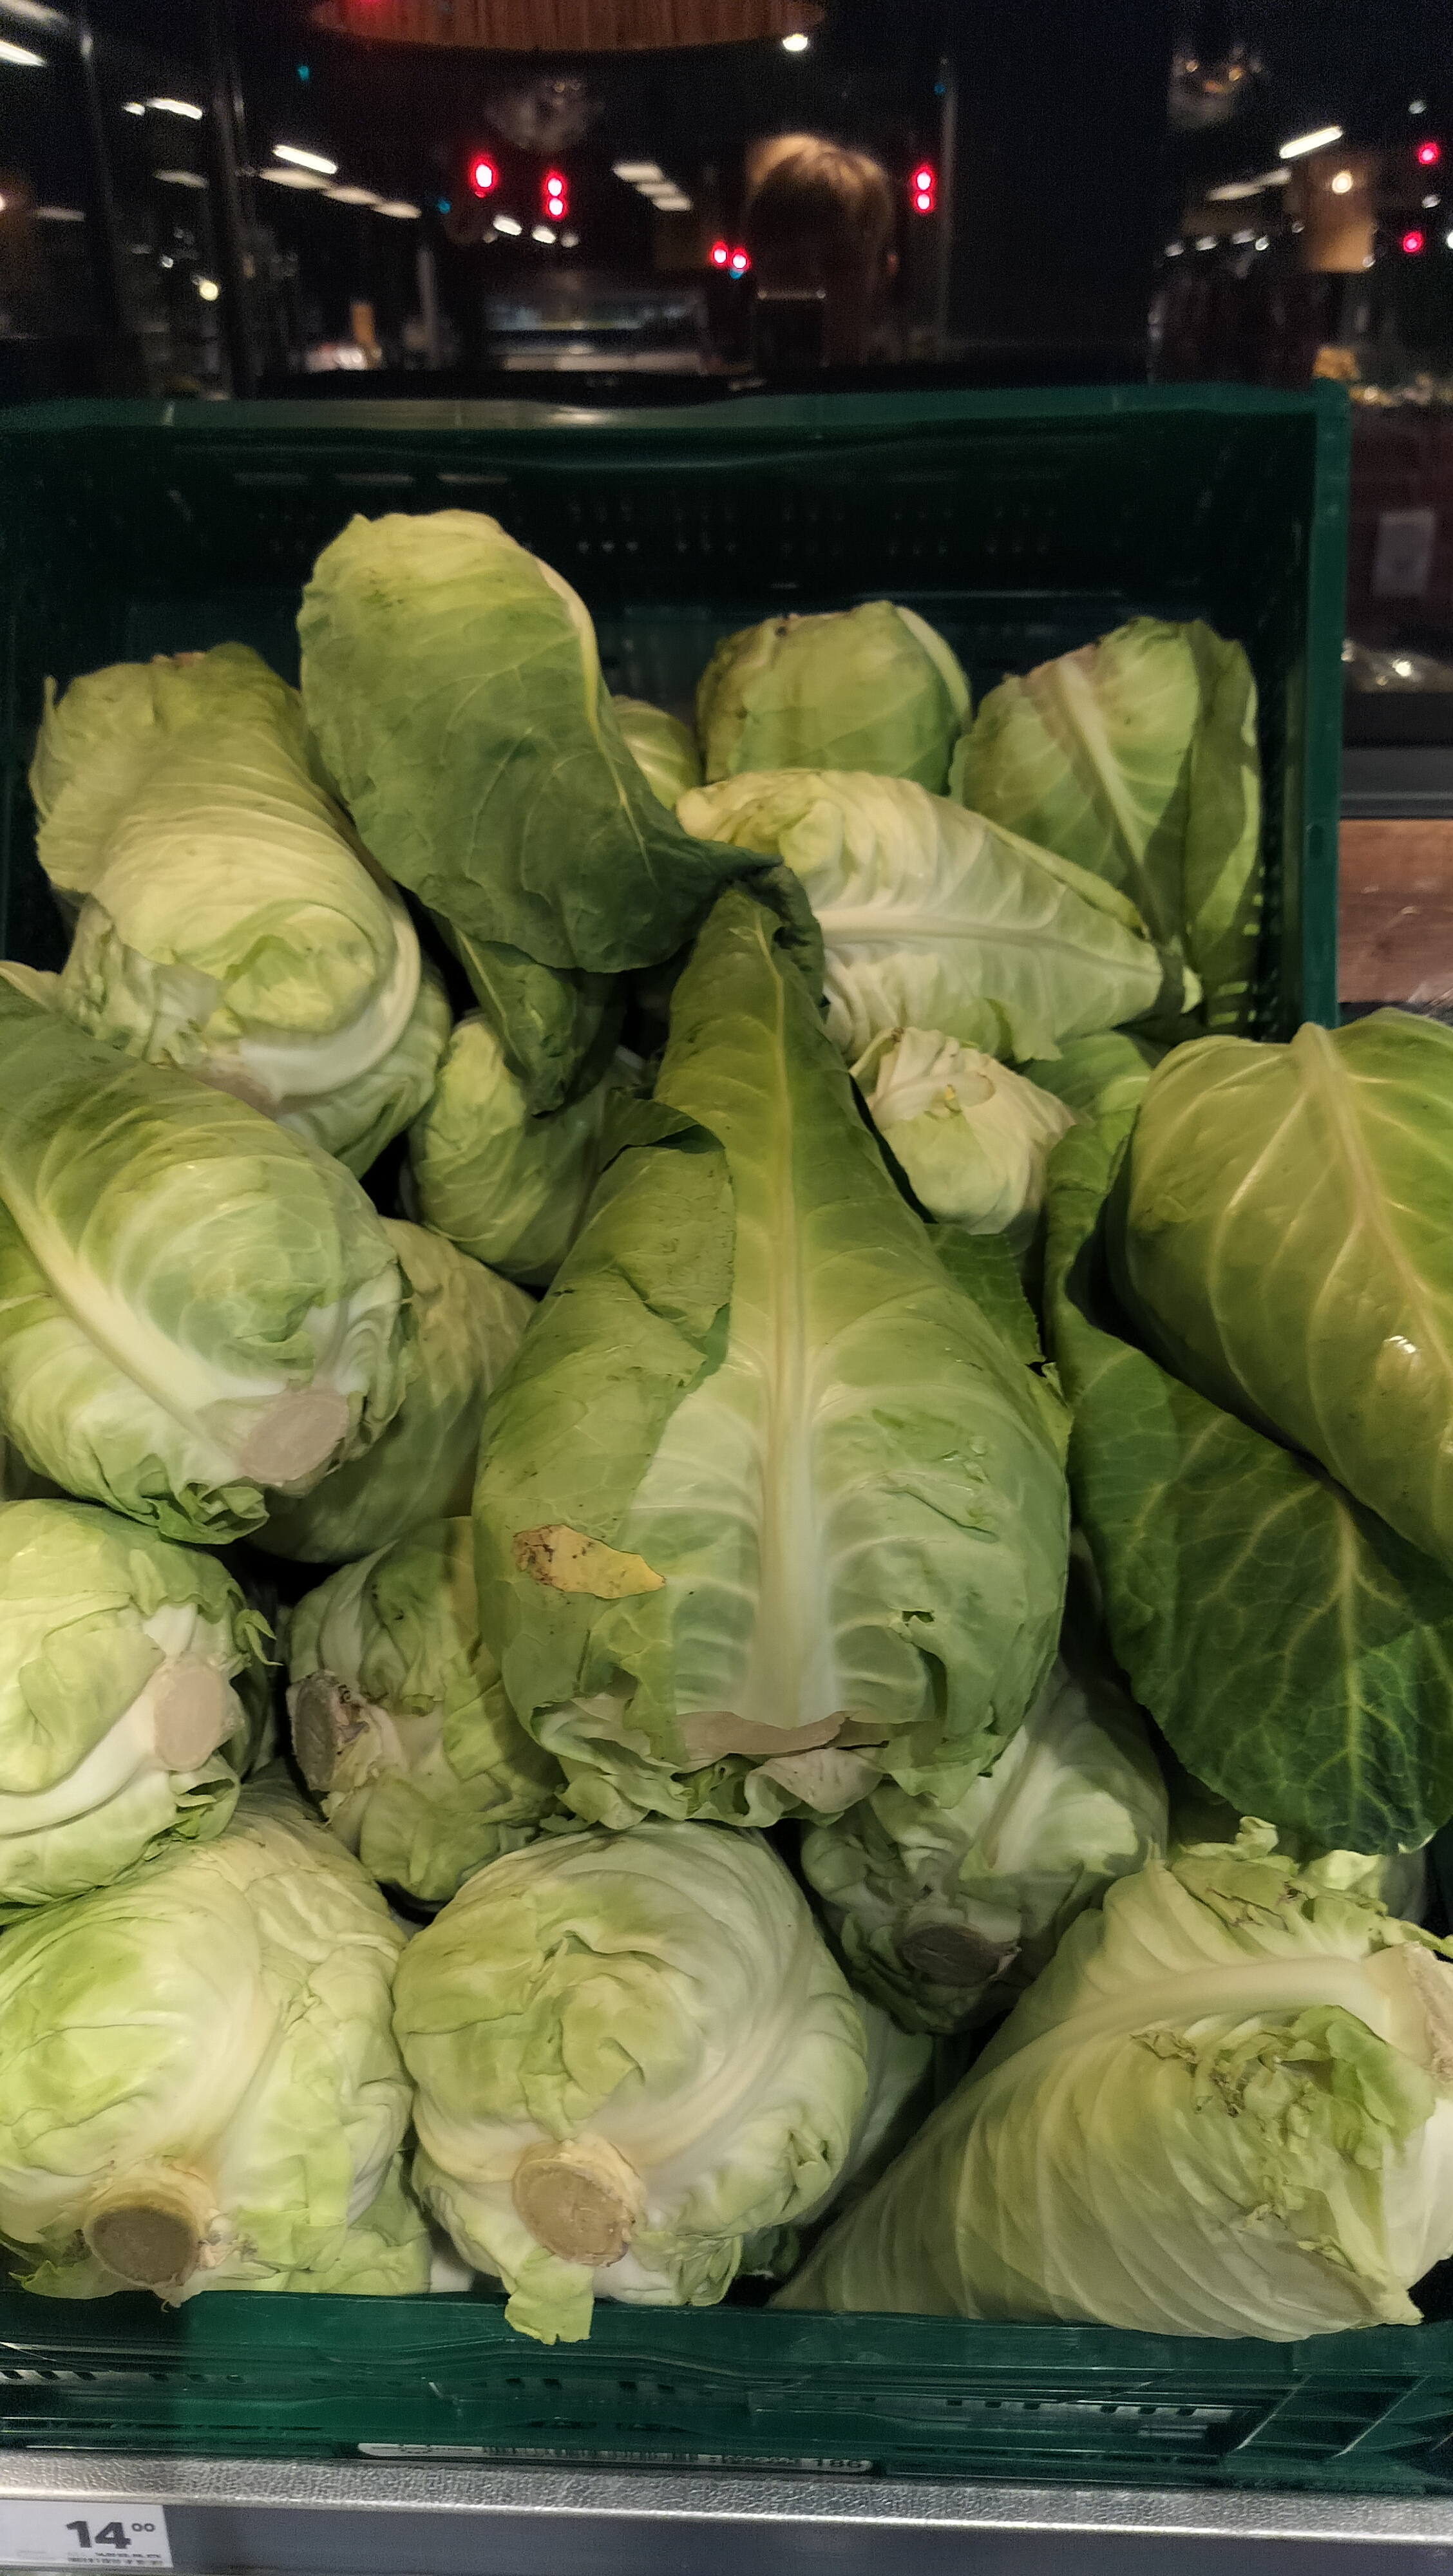
\includegraphics[width=0.5\linewidth]{Spidskål.jpg}
    \caption{Spidskål}
\end{figure}
% \chapter{Drinks}

\end{document}
